\documentclass[10pt,a4paper]{article}
\usepackage{fontspec}
\usepackage[spanish,es-noshorthands]{babel}
\usepackage[margin=2.2cm]{geometry}
\usepackage{amsmath,amssymb,booktabs,graphicx,siunitx,xcolor,caption,subcaption,array,microtype}
\usepackage{tikz}
\usepackage{adjustbox}
\usepackage{longtable}
\usepackage{float}
\usetikzlibrary{positioning,arrows.meta}
\usepackage{xurl}
\usepackage{hyperref}
\usepackage[natbibapa]{apacite}
\renewcommand{\doiprefix}{https://doi.org/\ignorespaces}% APA 7: DOI como enlace
\AtBeginDocument{\renewcommand{\BRetrievedFrom}{}}% APA 7: URL sin «Descargado de»

\sisetup{
  output-decimal-marker={,},
  group-separator={\,},
  group-digits=integer,
  group-minimum-digits=4,
  range-phrase={--},
  range-units=single,
  list-final-separator={ y },
  list-pair-separator={ y }
}
\hypersetup{colorlinks,linkcolor=teal,citecolor=teal,urlcolor=teal,pdftitle={Reconstrucción numérica del aluvión de San Carlos de Apoquindo (Las Condes, 8 de octubre de 2026)},pdfauthor={Lester Wood},pdflang={es-CL},pdfsubject={Simulación de flujo de barro; estudio cerrado el 13 de octubre de 2026}}
\captionsetup{font=small,labelfont=bf}
\graphicspath{{figs/}}
\newcommand{\Cvt}{C_{v,\mathrm{tot}}}% concentración volumétrica total de sólidos (densidad y balance de mezcla)
\newcommand{\Cvf}{C_{v,\mathrm{f}}}% concentración volumétrica de la matriz fina (relaciones reológicas)

\title{Reconstrucción numérica del aluvión de San Carlos de Apoquindo\\(Las Condes, 8 de octubre de 2026):\\recorrido, volumen e incertidumbre a partir de evidencia pública}
\author{Lester Wood\thanks{Estudio independiente. Contenido bajo licencia CC BY-NC-SA 4.0. Condiciones de uso: \url{https://aluvion.hirely.cl/terminos.html}.}}
\date{Estudio cerrado el 13 de octubre de 2026}

\begin{document}
\maketitle

\begin{abstract}
Según la prensa consultada, el 8 de octubre de 2026 un flujo de barro descendió desde la quebrada de San Carlos de Apoquindo (Las Condes, Santiago) sobre una ladera quemada nueve meses antes. Se ensayó su reconstrucción con un modelo bidimensional de aguas someras con reología de barro, sobre un relieve de \SI{30}{m} remuestreado a una retícula de \SI{4}{m} con 42.018 edificios, usando solo datos públicos y un registro probatorio de cada fuente consultada. Se completaron 84 simulaciones: 19 de cribado, 41 de ciudad completa, 5 de cuadratura y 19 microsimulaciones del campus. Con unos \SI{144}{mm} acumulados según lo informado por la alcaldesa y con la isoterma de \SI{0}{\celsius} informada por el CR2 por sobre la cumbre de la cuenca (área calculada: \SI{10,1}{km^2}), una estimación independiente que adopta la saturación del suelo informada sitúa el volumen de mezcla en unos \SI{295000}{m^3}, del mismo orden de magnitud que el requerido por el alcance simulado. La hipótesis seleccionada para la prueba reservada (z02) ---cauce principal, brazos sur y lluvia sobre la ladera--- reproduce los corredores de Camino El Alba, General Blanche y Quebrada Honda que delimitan la zona afectada oficial, el alcance hasta Padre Hurtado y cerca de \SI{1}{m} de barro en la Clínica UC Christus, con un índice exploratorio de compatibilidad (IEC) de 72/100. Este índice compara hipótesis y no mide precisión predictiva. Una prueba con observaciones reservadas, definida antes de examinar los resultados, resultó desfavorable: el flujo simulado alcanza 19 de 49 equipamientos afectados oficiales (\SI{39}{\percent}, frente al \SI{70}{\percent} fijado), porque el modelo deja sin barro partes de la zona afectada oficial. En los ensayos posteriores de ajuste, la entrada de barro en las casas representadas y el supuesto de agua turbia en el campus y La Plaza Sur, junto con barro en la rama principal, elevan el IEC verificado con paso fino a 76--82/100. La hipótesis integrada obtiene 79--82/100: 82 con la lluvia supuesta de \SI{35}{mm/h} y paso fino (z32), 81 con la lluvia medida en Río Molina con su forma de pulso (p34b, corregida) y 79 con esa lluvia repartida en \SI{4}{h} (v33). La severidad del incendio, estimada con Sentinel-2, muestra señal de quema en el \SI{82}{\percent} de las cuencas, en su mayoría con severidad baja o moderada-baja. Con los coeficientes supuestos para el escenario sin incendio, el balance calcula alrededor del \SI{62}{\percent} del volumen de barro y el \SI{43}{\percent} de los sólidos del escenario con incendio. En el modelo, un obstáculo supuesto de troncos al final del cauce principal no desvía el flujo hacia el sur. En escenarios hipotéticos, la inundación de Quebrada Honda se reproduce si el sumidero que representa el colector de Francisco Bulnes Correa no retira todo el flujo calculado en su embocadura, de unos \SI{65}{m^3/s}. Una capacidad supuesta de \SI{30}{m^3/s} deja flujo en superficie. Estos valores no describen la obra real. La retención en las casas representadas mejora la coincidencia con la zona afectada oficial, pero ninguna configuración reproduce a la vez esa extensión y el metro informado en la Clínica UC Christus. Las microsimulaciones y la simulación de ciudad con malla fina en el campus (m36) reproducen la entrada por el claro al patio hundido; m36 calcula \SI{0,17}{m} en el patio y moja el \SI{58}{\percent} de La Plaza Sur. El estudio se cerró el 13 de octubre de 2026; sus resultados de ajuste no tienen validación independiente.

\par\medskip\noindent\fbox{\parbox{0.96\linewidth}{\small\textbf{Declaración de alcance.} Estudio técnico independiente, de carácter académico, sin carácter oficial y basado exclusivamente en información pública. No es un peritaje ni evalúa obras, servicios o decisiones de personas o instituciones. Se distinguen tres tipos de resultados: \emph{observados} (lo informado por autoridades, prensa y cartografía oficial, siempre atribuido), \emph{calculados} (respuestas del modelo a parámetros de entrada declarados, como volúmenes y caudales) y \emph{escenarios hipotéticos} (variantes ensayadas, como capacidades supuestas del colector). Ningún valor calculado o hipotético es una medición, ninguna frase afirma la causa del evento ni atribuye responsabilidades, y todos los resultados requieren validación independiente. El estudio se cerró el 13 de octubre de 2026 (sección~\ref{sec:conclusiones}).}}
\end{abstract}

\section{Introducción y planteamiento del problema}\label{sec:intro}
Según las fuentes periodísticas citadas, el jueves 8 de octubre de 2026, cerca de las 17:00 (UTC$-$3), un flujo de agua, barro y rocas descendió desde la quebrada que drena el sector precordillerano de San Carlos de Apoquindo (Las Condes, Santiago) y recorrió calles residenciales por varios kilómetros. Arrastró vehículos y un bus \citep{theclinic2026frontal}, inundó viviendas, una clínica y una universidad, dejó seis heridos y motivó la declaración de zona de catástrofe \citep{interferencia2026}. Según la información periodística consultada, que recoge antecedentes del Servicio Nacional de Geología y Minería (Sernageomin), el evento ocurrió en una zona clasificada en febrero de 2026 como de alto peligro por flujos de detritos \citep{chilevision2026}. Según el municipio y BioBioChile, la cuenca había sido afectada por un incendio de unas \SI{1000}{ha} entre diciembre de 2025 y enero de 2026 \citep{lascondes2026,biobio2026origen}. Según el CR2, el evento siguió a un comienzo de octubre excepcionalmente lluvioso: más de \SI{90}{mm} en Quinta Normal en lo que iba del mes, cerca del máximo histórico de octubre de 1930 \citep{cr2_2026}.

Al día siguiente, entre las fuentes públicas consultadas no se había localizado una cartografía oficial del área afectada, ni aforos, ni marcas de nivel publicadas. La información disponible se reducía a notas de prensa, la lista de calles cerradas por el municipio, un perímetro de afectación y dos versiones de las fuentes sobre el origen que no coinciden entre sí. Este trabajo ensaya escenarios de recorrido, volumen y caudal del aluvión mediante un modelo físico explícito y evidencia pública verificable. Asimismo, calcula para esos escenarios la profundidad, la velocidad y la presión del flujo en calles y edificios del área de estudio, considerando la incertidumbre de las estimaciones.


\IfFileExists{secciones/relato.tex}{\section{Relato de los hechos}\label{sec:relato}
Esta sección reconstruye en orden cronológico lo informado por organismos públicos, investigadores y prensa, con cada dato atribuido a su fuente. Las horas son locales (UTC$-$3) y aproximadas. Cuando las fuentes difieren, se presentan todas las versiones, sin resolverlas.

\subsection*{Antecedentes}
\paragraph{La cuenca y el abanico.} Según el análisis del Centro de Ciencia del Clima y la Resiliencia (CR2), Quebrada Honda drena una cuenca pequeña de la precordillera, de unos \SI{10,6}{km^2} y entre \SI{929}{m} y \SI{2355}{m} de altitud, que desemboca en el límite urbano de Santiago \citep{cr2_2026}. Según La Tercera, al pie se extiende el barrio de San Carlos de Apoquindo, donde se concentran colegios, clínicas y universidades \citep{latercera2026zonacero}. El decano de Arquitectura de la Universidad del Desarrollo, citado por El Desconcierto, explicó que varias quebradas de la ladera confluyen en un solo cauce y que «la quebrada se entuba en Bulnes Correa y el problema con los colectores cerrados es que tienen capacidad limitada» \citep{eldesconcierto2026}. Según dijo a The Clinic, ese cauce corre por un parque junto a General Blanche y, ya entubado, sigue bajo la calle Quebrada Honda \citep{theclinic2026allard}.

\paragraph{El incendio.} Según el CR2, el 29 de diciembre de 2025 comenzó un incendio en la cuenca \citep{cr2_2026}. El municipio informó que partió en el sector La Plaza Sur, que afectó una superficie preliminar de \SI{1012}{ha} en la comuna y que Conaf lo dio por controlado la tarde del 1 de enero \citep{lascondes2026}. Las cifras de superficie varían: «cerca de 1.000 hectáreas» según el CR2, que agrega que el fuego comprometió prácticamente toda la cuenca \citep{cr2_2026}; «aproximadamente mil hectáreas» en cuatro días según T13 \citep{t13_2026mallas}; y «más de 800 hectáreas», con el fuego a \SI{200}{m} de zonas urbanas, según Interferencia \citep{interferencia2026}. Según el cálculo de este estudio (sección~\ref{sec:res-incendio}), \SI{8,2}{km^2} de los \SI{10,1}{km^2} de las cuencas aportantes muestran señal de quema, con severidad mayoritariamente baja o moderada-baja.

\paragraph{El evento del 31 de enero.} Según el reporte de Sernageomin, ese día se activaron las quebradas La Honda, Grande, Los Almendros y Apoquindo \citep{sernageomin2026reterm}. Según T13, cayeron \SI{75}{mm} en una hora y \SI{20}{min}, y el evento afectó ocho hectáreas urbanas, casi \SI{4}{km} de calles y 11 viviendas \citep{t13_2026mallas}. Interferencia, en cambio, menciona «apenas 20 minutos de lluvia intensa» \citep{interferencia2026}. El Mostrador cifra en 22 las viviendas dañadas, según antecedentes iniciales de Senapred \citep{elmostrador2026}. La alcaldesa de Las Condes dijo entonces, según La Tercera, que el colector de Francisco Bulnes Correa «funcionó muy bien», aunque hubo puntos afectados, como las calles Mirasol y Carlos Peña \citep{latercera2026enero}.

\paragraph{La advertencia de Sernageomin.} Según el propio reporte, tras un sobrevuelo del 6 de febrero el Servicio Nacional de Geología y Minería elaboró el 11 de febrero el Reporte Técnico de Remoción en Masa Metropolitana 02/2026 \citep{sernageomin2026reterm}. Según Chilevisión, el informe situó el área en una zona de «alto peligro» por flujos de detritos e inundaciones, identificó flujos en las quebradas La Honda, Grande y Apoquindo, y señaló «deficiencias en las obras de mitigación y adecuación» \citep{chilevision2026}. El reporte de Sernageomin concluyó que el evento de enero «no constituye una ocurrencia aislada, sino una reactivación de procesos en un área altamente propensa» a estos fenómenos \citep{sernageomin2026reterm}. Según Chilevisión, el reporte recomendó, entre otras medidas, planes de evacuación y la limpieza periódica de los cauces \citep{chilevision2026}.

\paragraph{Las obras de mitigación.} Según Interferencia, el 26 de marzo la alcaldesa pidió al delegado presidencial instalar mallas dinámicas; él reconoció que sería difícil tenerlas antes de mayo \citep{interferencia2026}. Según el mismo medio, el 7 de agosto se anunció un convenio para cinco barreras con \$754 millones del Ministerio de Obras Públicas (MOP) y un plazo de 90 días \citep{interferencia2026}. T13 informa otra cifra: un contrato por trato directo de \$652 millones, firmado en septiembre, también a 90 días \citep{t13_2026mallas}. Según Interferencia, durante la emergencia el delegado presidencial confirmó que aún no estaban listas \citep{interferencia2026}.

\subsection*{La lluvia}
Según el CR2, un río atmosférico de categoría 2 a 3 alcanzó la zona central el 6 y el 7 de octubre. Dejó \SI{72}{mm} en Quinta Normal y cerca de \SI{100}{mm} en la precordillera de Santiago \citep{cr2_2026}. El 8 persistía una baja segregada estacionaria a unos \SI{5}{km} de altura que, según el CR2, junto con la humedad del río atmosférico, generó núcleos convectivos con oscurecimiento repentino, rayos, granizo y lluvia intensa en periodos de \SIrange{30}{60}{min} \citep{cr2_2026}. El CR2 señala que no parece haber pluviómetros en la cuenca; en la estación Río Molina, a unos \SI{7}{km}, cayeron \SI{42,8}{mm} ese día, \SI{31,6}{mm} de ellos entre las 15:00 y las 19:00, con un máximo de \SI{10,9}{mm} en \SI{30}{min}. Según ese análisis, la isoterma de \SI{0}{\celsius} se situó a unos \SI{2800}{m}, de modo que toda la cuenca recibió lluvia y no nieve \citep{cr2_2026}. Según el CR2, los rayos llegaron al nororiente de Santiago y a Las Condes cerca de las 16:30, y hacia las 17:00 se localizaban sobre todo en el Cajón del Maipo \citep{cr2_2026}. En Tobalaba, la Dirección Meteorológica de Chile registró \SI{34,8}{mm} el día 8 y \SI{13,8}{mm} entre las 15:00 y las 21:00 \citep{dmc2026}.

Otras cifras circularon sin medición identificada. La alcaldesa habló de \SI{144}{mm} acumulados, \SI{20}{mm} de ellos ese día, con el suelo saturado \citep{interferencia2026}. Según la versión consultada de Wikipedia, el subsecretario del Interior mencionó unos \SI{15}{mm} en un intervalo muy breve \citep{wikipedia2026}. Búsquedas en prensa registradas el 9 de octubre devolvieron también cifras de \SI{16}{mm} a \SI{20}{mm} en alrededor de una hora, sin estación identificada. La cifra de \SI{27}{mm} en \SI{20}{min} no se encontró en la prensa consultada y no está verificada. Los \SI{25}{mm} que también circularon parecen corresponder a un pronóstico para el 11 al 13 de octubre difundido por Canal 9, no a la lluvia caída el día 8 (búsqueda registrada el 12 de octubre).

\subsection*{El aluvión}
Cerca de las 17:00, según información preliminar de Carabineros, se divisó un «gran torrente de agua por calle General Blanche», que esa información atribuía al rebalse del canal de la calle Francisco Bulnes Correa; el caudal bajó hacia el poniente \citep{theclinic2026frontal,eldesconcierto2026}. Las fuentes ubican el inicio en puntos distintos. La Tercera informó que «todo comenzó al activarse una quebrada a la altura de General Blanche con San Carlos de Apoquindo», con avance hacia el surponiente \citep{latercera2026}. Según La Tercera, Carabineros, con un dron, ubicó la «zona cero» en Mons.\ Álvaro del Portillo con Av.\ La Plaza \citep{latercera2026zonacero}. Según Chilevisión, las autoridades atribuyeron el evento a la activación de la «Quebrada Las Ondas» \citep{chilevision2026mapa}, mientras Chilevisión, a partir del informe de Sernageomin, y el CR2 hablan de la quebrada La Honda u Honda \citep{chilevision2026,cr2_2026}.

El vicerrector de Comunicaciones de la Universidad de los Andes relató a Cooperativa un desborde de la quebrada en el lado norte del campus, que colinda con General Blanche, «por donde cayó toda esta masa de barro» \citep{cooperativa2026}. Según El Desconcierto, el flujo arrastró autos y un bus del sistema RED, cuyos pasajeros debieron subir al techo \citep{eldesconcierto2026}. La Tercera y T13 informaron que el bus fue volcado \citep{latercera2026,t13_2026vehiculos}; Cadena 3, que un vehículo de transporte público logró detenerse \citep{cadena3_2026}. Según el municipio, el barro bajó por Camino El Alba, General Blanche y Quebrada Honda \citep{latercera2026,chilevision2026mapa}. Según El Dínamo, Senapred señaló como más afectadas General Blanche, Quebrada Honda y la Av.\ La Plaza Sur \citep{eldinamo2026}. Según T13, el agua se acumuló también en la Av.\ Padre Hurtado \citep{t13_2026vehiculos}.

En la Clínica UC Christus, Cadena 3 informó cerca de \SI{1}{m} de barro en el servicio de urgencias \citep{cadena3_2026}. Según El Desconcierto, se suspendió la atención en ese servicio y las consultas \citep{eldesconcierto2026}. Según BioBioChile, en la sede del Duoc UC estudiantes y trabajadores quedaron atrapados en un auditorio \citep{biobio2026duoc}. Según Cooperativa, la comunidad de la Universidad de los Andes permaneció en el campus por recomendación de Bomberos \citep{cooperativa2026}. Un video difundido en Facebook se titula «Aluvión ingresó hasta el aula Magna de la Universidad de Los Andes» \citep{quintaconectado2026}, y Meganoticias publicó a las 18:16 imágenes del campus inundado \citep{meganoticias2026uandes}. Interferencia informó además agua y barro en el Hospital de la FACh \citep{interferencia2026}.

Sobre el drenaje se informaron versiones distintas, todas preliminares. Según Chilevisión, el delegado presidencial presumió «el bloqueo, el taponeo del canal subterráneo» en Álvaro del Portillo con Av.\ La Plaza \citep{chilevision2026}. Según Interferencia, en otra declaración el delegado apuntó a la obstrucción de dos ductos en General Blanche \citep{interferencia2026}. Según El Desconcierto, el canal entubado que baja desde la Av.\ La Plaza llega a una cámara de decantación en Francisco Bulnes Correa y, «con ese sistema colapsado, la calle funcionó como el nuevo cauce» \citep{eldesconcierto2026}. Interferencia subrayó que era una hipótesis sin confirmación técnica \citep{interferencia2026}.

\subsection*{Consecuencias y respuesta}
\paragraph{La tarde y la noche del 8.} Según Interferencia, Senapred dio su primer aviso público a las 17:41, con un video de su director regional; no envió un mensaje de evacuación a los celulares \citep{interferencia2026}. La alerta roja para diez comunas rigió desde las 18:20 según Interferencia \citep{interferencia2026}; La Tercera la sitúa a las 18:30 \citep{latercera2026lluvias}. Según La Tercera, a las 18:15 el presidente de la República escribió que se enfrentaba «una emergencia de activación muy rápida» \citep{latercera2026lluvias}. Según Interferencia, esa noche el presidente instruyó decretar zona de catástrofe tras un comité regional de gestión del riesgo \citep{interferencia2026}; según la versión consultada de Wikipedia, la medida se formalizó el 9 de octubre \citep{wikipedia2026}. El delegado presidencial informó, según Interferencia y El Desconcierto, seis lesionados, entre ellos un niño de un año con una fractura, y ningún fallecido \citep{interferencia2026,eldesconcierto2026}. Según Chilevisión, el ministro del Interior anunció un polígono de exclusión de ingreso tras un reconocimiento aéreo \citep{chilevision2026mapa}. Pasadas las 23:00, la alcaldesa dijo a Cooperativa que «el cerro cedió de manera casi completa» \citep{cooperativa2026alcaldesa}.

\paragraph{El perímetro.} Según The Clinic, el primer perímetro municipal de seguridad iba de Camino El Alba a Quebrada Honda, con Vital Apoquindo y el límite cordillerano por el oriente, sujeto a ajustes \citep{theclinic2026frontal}. Según La Tercera, el polígono informado después tenía por límites Camino El Alba (norte), la Av.\ La Plaza (oriente), Quebrada Honda (sur) y la Av.\ Padre Hurtado (poniente), en el sector del Pueblito Los Dominicos \citep{latercera2026}.

\paragraph{Superficie y viviendas.} Las cifras difieren según el organismo y la fecha:
\begin{itemize}
\item Superficie: unas \SI{200}{ha} según el balance de la noche del 8 \citep{wikipedia2026}; \SI{253}{ha} y 3.981 roles de avalúo según la plataforma inmobiliaria Inciti \citep{chicureohoy2026}; \SI{288,5}{ha}, 2.266 predios y 368 tramos de calle en el visor oficial de IDE Chile \citep{bbnn2026visor}.
\item Municipalidad (9 de octubre): 2.015 viviendas afectadas, 55 inhabitables y 1.960 con daños menores, según CNN Chile y Chicureo Hoy \citep{cnnchile2026balance,chicureohoy2026}. Ese mismo día, el delegado presidencial habló de 1.960 viviendas afectadas, 55 de ellas con «problemas serios de habitabilidad», según Publimetro \citep{publimetro2026}.
\item Senapred: 75 viviendas con daño mayor y 2.286 con daño menor el 9 de octubre, según La Tribuna \citep{latribuna2026}; más tarde, según La Tercera, 56 destruidas, 40 con daño mayor, 1.960 con daño menor y 384 damnificados \citep{latercera2026senapred}.
\item Visor de Bienes Nacionales: 22 viviendas con daño mayor, 1.960 con daño menor y 51 equipamientos afectados \citep{bbnn2026visor}.
\end{itemize}
La municipalidad cifró en 1.200 las personas evacuadas o rescatadas, según CNN Chile \citep{cnnchile2026balance}.

\paragraph{La Clínica Universidad de los Andes.} Las versiones no coinciden. Meganoticias informó que el barro ingresó hasta el área de urgencias \citep{meganoticias2026urgencia}, y BioBioChile difundió imágenes de salas y pasillos anegados atribuidas a esta clínica y a la Clínica UC Christus \citep{biobio2026clinicas}. La directora de Comunicaciones de la clínica afirmó a Radio La Señal que «toda la afectación fue en el exterior» y que solo entró «un poco de agua en una sala de espera», de no más de un centímetro \citep{radiolasenal2026}. El balance municipal consignó «un ingreso menor de agua», con la urgencia disponible, según CNN Chile \citep{cnnchile2026balance}.

\paragraph{Las mallas.} Según T13, el 9 de octubre el ministro de Obras Públicas dijo que había habido «instalaciones de mallas dinámicas». La alcaldesa precisó luego que faltaba habilitar los accesos y que la instalación «partía mañana»; el ministro reconoció después que los trabajos estaban en una etapa previa \citep{t13_2026mallas}. Según Chicureo Hoy, el Ministerio Público abrió una investigación sobre eventuales responsabilidades penales \citep{chicureohoy2026}.

\subsection*{Preguntas que dejan los hechos}
No hay acuerdo sobre el punto por donde el flujo salió a la ciudad: Álvaro del Portillo con La Plaza, General Blanche con San Carlos de Apoquindo o el canal de Francisco Bulnes Correa. Tampoco está establecido si el barro provino de un solo cauce o de varias quebradas, como sugirió a CNN Chile un concejal de Las Condes \citep{cnnchile2026haddad}. No se localizaron en las fuentes consultadas mediciones de la lluvia dentro de la cuenca ni del volumen movilizado, que el delegado presidencial describió como «miles de metros cúbicos» \citep{cooperativa2026alcaldesa}. Las superficies y conteos publicados difieren entre sí y ninguno informa espesores ni marcas de nivel. Estas preguntas motivan las hipótesis de la sección~\ref{sec:hipotesis}.
}{}

\section{Marco teórico}\label{sec:marco}
\paragraph{Flujos de detritos y de barro.} Un aluvión es una mezcla de agua y sedimento cuyo comportamiento depende de la concentración volumétrica total de sólidos $\Cvt$. Con $\Cvt$ entre $0{,}20$ y $0{,}55$ la mezcla presenta un esfuerzo de fluencia $\tau_y$: se detiene cuando el esfuerzo motriz no lo supera. Su densidad es $\rho_m=\rho_w+\Cvt(\rho_s-\rho_w)$, donde $\rho_m$, $\rho_w$ y $\rho_s$ son las densidades de la mezcla, el agua y los sólidos, respectivamente (\si{kg.m^{-3}}); $\rho_m$ se sitúa entre \SI{1300}{kg.m^{-3}} y \SI{1900}{kg.m^{-3}}. En las relaciones reológicas interviene, en cambio, la concentración de la matriz fina $\Cvf$ (sección~\ref{sec:modelo}).

\paragraph{Rangos de concentración y densidad en la literatura.} Las crecidas con barro y los flujos hiperconcentrados tienen entre un \SI{20}{\percent} y un \SI{45}{\percent} de sedimento en volumen, con promedios de \SI{20}{\percent} a \SI{35}{\percent} y picos cercanos al \SI{45}{\percent} en los flujos de barro \citep{obrien1988,flo2d2021}; su densidad queda entre unos \SI{1330}{kg.m^{-3}} y \SI{1740}{kg.m^{-3}}. Sobre un \SI{50}{\percent} en volumen se habla de flujo de detritos \citep{costa1984,zanuttigh2007}, con concentraciones de sólidos de \SI{50}{\percent} a \SI{80}{\percent} y densidades de \SI{1400}{kg.m^{-3}} a \SI{2400}{kg.m^{-3}} medidas en canales experimentales y en muestras naturales \citep{iverson1997}; en oleadas densas observadas en terreno se han estimado unos \SI{2000}{kg.m^{-3}} \citep{zanuttigh2007}. La tabla~\ref{tab:densidades} sitúa en ese marco los barros ensayados en este estudio.

\begin{table}[htbp]\centering\small
\caption{Concentración volumétrica de sedimento ($C_v$) y densidad de la mezcla según la literatura, y barros ensayados en este estudio. Las densidades de los barros ensayados se calculan con $\rho_s=\SI{2650}{kg.m^{-3}}$; $\tau_y$ y $\eta$ son la fluencia y la viscosidad de la matriz fina según \citet{obrien1988}.}\label{tab:densidades}
\begin{adjustbox}{max width=\textwidth}\begin{tabular}{lll}\toprule
Tipo de flujo o barro & $C_v$ & $\rho_m$ (\si{kg.m^{-3}})\\\midrule
Crecida con barro y flujo hiperconcentrado \citep{obrien1988,flo2d2021} & 0,20--0,45 & \numrange{1330}{1740}\\
Flujo de barro, valores típicos \citep{flo2d2021} & 0,20--0,35 (picos de 0,45) & \numrange{1330}{1740}\\
Umbral de flujo de detritos \citep{costa1984,zanuttigh2007} & $\geq0{,}50$ & $\geq\num{1825}$\\
Flujo de detritos \citep{iverson1997} & 0,50--0,80 & \numrange{1400}{2400}\\\midrule
Este estudio: Glenwood~2b ($\tau_y=\SI{6,6}{Pa}$, $\eta=\SI{0,77}{Pa.s}$) & 0,40 & \num{1660}\\
Este estudio: Glenwood~2b con $C_v=0{,}43$ ($\tau_y\approx\SI{11}{Pa}$) & 0,43 & \num{1710}\\
Este estudio: Glenwood~1 ($\tau_y=\SI{29}{Pa}$, $\eta=\SI{8,8}{Pa.s}$) & 0,45 & \num{1742}\\
\bottomrule\end{tabular}\end{adjustbox}
\end{table}

\paragraph{Elección del barro y su motivo.} Tres evidencias orientan la elección. Según BioBioChile, Sernageomin clasificó el evento como una crecida repentina que arrastró gran cantidad de sedimento \citep{biobio2026origen}; en las imágenes del día consultadas se interpreta una matriz fina con piedras, troncos y vehículos arrastrados, sin frentes de bloques visibles; y el alcance observado, hasta la Av.\ Padre Hurtado, exige un barro capaz de recorrer varios kilómetros por calles de baja pendiente. Para el modelo se adopta un rango entre el extremo alto de los flujos de barro y el umbral de los flujos de detritos. El barro de referencia (Glenwood~2b, $C_v=0{,}40$) está en ese rango; en las simulaciones, uno más espeso (Glenwood~1, $C_v=0{,}45$) se detiene antes de Padre Hurtado, y el de referencia se extiende más allá de la zona afectada oficial. Como la fluencia crece exponencialmente con la concentración \citep{obrien1988}, un cambio pequeño ---de 0,40 a 0,43--- casi duplica $\tau_y$; por eso se ensayó ese valor intermedio, que además representa la resistencia adicional de la carga gruesa (piedras, troncos y escombros) que la reología de la matriz fina no incluye.

\paragraph{Aguas someras con reología.} Cuando el espesor del flujo es pequeño frente a su extensión, las ecuaciones de Navier–Stokes integradas en la profundidad se reducen a las de Saint-Venant en dos dimensiones. La reología de la mezcla entra como una pendiente de fricción $S_f$, definida en la ecuación~\eqref{eq:friccion}. El cierre cuadrático de \citet{obrien1988} y \citet{obrien1993}, usado por FLO-2D \citep{flo2d2021}, suma tres términos: fluencia, viscosidad y turbulencia más colisión de granos.

\paragraph{Representación urbana.} En ciudad, el flujo se canaliza por las calles y lo desvían los edificios. Estos pueden representarse como bloques elevados, como huecos impermeables o mediante porosidad; la elección condiciona la capacidad predictiva \citep{schubert2012}.

\paragraph{Volumen movilizable.} El volumen de un flujo de detritos puede estimarse con un balance entre lluvia y escorrentía. En cuencas recién quemadas existen además modelos empíricos que lo relacionan con la intensidad de lluvia de \SI{15}{min}, el área quemada y el relieve \citep{gartner2014}. El caudal pico se relaciona empíricamente con el volumen \citep{mizuyama1992}.

\paragraph{Calibración con observaciones cualitativas.} Cuando solo se conoce la extensión del área afectada, distintas combinaciones de volumen, caudal y resistencia producen huellas parecidas, es decir, hay equifinalidad. El enfoque de estimación de incertidumbre mediante verosimilitud generalizada (GLUE, por sus siglas en inglés; \citealp{beven1992}) propone aceptar todas las simulaciones de comportamiento aceptable e informar la envolvente de sus predicciones en lugar de un único mejor ajuste.


\section{Hipótesis y objetivos}\label{sec:hipotesis}
\paragraph{Hipótesis de entrada al modelo.} Se contrastaron tres configuraciones hipotéticas de localización de los aportes del flujo a la zona urbana, formuladas a partir de fuentes de distinta confiabilidad; no identifican el origen ni el estado de las obras durante el evento:
\begin{description}
\item[H1] Se ensayó una entrada superficial de todo el flujo en el abanico, en las calles Mons.\ Álvaro del Portillo, Av.\ La Plaza y General Blanche, sin ingreso al ducto en el modelo. La ubicación se basa en las versiones recogidas por Chilevisión e Interferencia \citep{chilevision2026,interferencia2026}.
\item[H2] Se ensayó una entrada superficial en el cruce del cauce entubado con la calle Francisco Bulnes Correa, al inicio de Quebrada Honda. La ubicación se basa en las versiones recogidas por Interferencia y BioBioChile \citep{interferencia2026,biobio2026origen}.
\item[H3] Se supuso un aporte distribuido en varios puntos donde los cauces de la precordillera llegan a la urbanización: el cauce principal (H1), un cauce sur que cruza el campus de la Universidad de los Andes (S1) y quebradas menores que terminan en la Av.\ La Plaza Sur (S2). El hidrograma se reparte en proporción al área de cada cuenca.
\end{description}
Durante el estudio se agregaron, como hipótesis \emph{exploratorias} formuladas después de examinar los primeros resultados, H4 (salida combinada en el abanico y en la embocadura del colector de Francisco Bulnes Correa, más los aportes del sur) y H5 (H4 más escurrimiento directo de lluvia sobre la ladera oriente de La Plaza Sur). También se ensayaron dos representaciones del terreno (el cauce del parque lineal tallado y un terreno fotogramétrico de mayor resolución) y distintas capacidades supuestas del colector. Se informan separadas de las hipótesis iniciales.
\paragraph{Hipótesis de proceso (HP).} Un modelo bidimensional de aguas someras con reología de mezcla homogénea, alimentado con un volumen compatible con la lluvia observada, reproduce la extensión informada: las calles con presencia de barro y el alcance hasta la Av.\ Padre Hurtado.

\paragraph{Objetivo general.} Estimar el recorrido del aluvión y los indicadores hidrodinámicos en calles y edificios, y caracterizar su incertidumbre a partir del conjunto de simulaciones aceptables.

\paragraph{Objetivos específicos.}
\begin{enumerate}
\item Construir un terreno urbano con edificios y calles a partir de datos abiertos.
\item Implementar y verificar la reología de la mezcla en un modelo bidimensional de código abierto.
\item Acotar el volumen de mezcla de forma independiente, con lluvia y modelos empíricos.
\item Calibrar el caudal, el volumen y la reología mediante la evidencia pública y comparar la compatibilidad de las hipótesis H1, H2 y H3 con las observaciones.
\item Cuantificar la incertidumbre y publicar los resultados de forma reproducible.
\end{enumerate}

\paragraph{Correspondencia entre hipótesis, objetivos, métodos y resultados.} La tabla~\ref{tab:correspondencia} vincula cada hipótesis y cada objetivo con el procedimiento que lo aborda y con el resultado informado al cierre.

\begin{table}[htbp]\centering\small
\caption{Correspondencia entre las hipótesis de entrada (H1, H2 y H3), la hipótesis de proceso (HP), los objetivos, los métodos y los resultados al cierre.}\label{tab:correspondencia}
\begin{tabular}{@{}>{\raggedright\arraybackslash}p{.27\textwidth}>{\raggedright\arraybackslash}p{.33\textwidth}>{\raggedright\arraybackslash}p{.33\textwidth}@{}}\toprule
Hipótesis u objetivo & Método correspondiente & Resultado informado\\\midrule
H1, H2 y H3, evaluadas por separado & Fuentes de entrada y criterios de calibración (secciones~\ref{sec:modelo} y~\ref{sec:calib}) & Cribado y métricas por hipótesis (secciones~\ref{sec:res-calib} y~\ref{sec:recorrido})\\
HP & Modelo y criterios de reproducción de la extensión (secciones~\ref{sec:modelo} y~\ref{sec:calib}) & Compatibilidad y prueba reservada (secciones~\ref{sec:res-ronda} y~\ref{sec:res-posterior})\\
Objetivo específico 1 & Construcción del terreno urbano (sección~\ref{sec:terreno}) & Ciudad completa y terreno anterior (secciones~\ref{sec:res-v4} y~\ref{sec:res-terreno})\\
Objetivo específico 2 & Implementación y verificación (secciones~\ref{sec:modelo} y~\ref{sec:verif}) & Resultados de parada, reinicio, convergencia y balance (sección~\ref{sec:res-verif})\\
Objetivo específico 3 & Estimación independiente del volumen (sección~\ref{sec:volumen}) & Distribuciones de volumen y severidad estimada (secciones~\ref{sec:res-volumen} y~\ref{sec:res-incendio})\\
Objetivo específico 4 & Calibración inversa (sección~\ref{sec:calib}) & Comparación H1--H3 y ajustes posteriores (secciones~\ref{sec:recorrido} y~\ref{sec:res-posterior})\\
Objetivo específico 5 & Síntesis de incertidumbre y publicación (sección~\ref{sec:sintesis}) & Cuadratura e incertidumbre (secciones~\ref{sec:res-posterior} y~\ref{sec:discusion}) y \hyperref[sec:versiones]{versiones reproducibles}\\
Objetivo general & Extracción de indicadores por calle y edificio (sección~\ref{sec:sintesis}) & Recorrido, indicadores y limitaciones (secciones~\ref{sec:recorrido},~\ref{sec:res-indicadores} y~\ref{sec:discusion})\\\bottomrule
\end{tabular}
\end{table}


\section{Metodología}\label{sec:metodo}
\begin{figure}[htbp]\centering
\begin{tikzpicture}[font=\footnotesize, x=36mm, y=-16mm,
  caja/.style={draw, rounded corners=2pt, align=center, minimum height=11mm, text width=30mm, fill=#1}, caja/.default=white,
  flecha/.style={-{Stealth[length=2mm]}, thick}]
\node[caja=blue!8] (reg) at (0,0) {Registro probatorio\\(fecha, fuente,\\huella SHA-256)};
\node[caja=blue!8] (obs) at (1,0) {Evidencia pública\\(prensa, municipio,\\Senapred, Sernageomin)};
\node[caja=blue!8] (dat) at (2,0) {Datos abiertos\\(terreno, edificios,\\calles, cauces, lluvia)};
\node[caja=orange!12] (hip) at (1,1) {H1--H3 iniciales;\\H4--H5 exploratorias;\\criterios previos};
\node[caja=orange!12] (ter) at (2,1) {Superficie de cálculo\\(terreno, bloques,\\calles, cauce)};
\node[caja=orange!12] (vol) at (3,1) {Volumen previo\\(lluvia × cuenca;\\cuencas quemadas)};
\node[caja=red!10] (ver) at (1,2) {Verificación numérica\\(parada, balance,\\convergencia)};
\node[caja=red!10] (sim) at (2,2) {Simulación 2D:\\aguas someras +\\reología de barro};
\node[caja=red!10] (rev) at (3,2) {Revisión automatizada\\con IA (física A1--A2;\\formato y redacción)};
\node[caja=green!12] (sat) at (1,3) {Contraste satelital\\independiente\\(no probado)};
\node[caja=green!12] (cal) at (2,3) {Evaluación frente a\\observaciones\\(calles y sitios)};
\node[caja=green!12] (res) at (3,3) {Resultados: recorrido,\\indicadores, nodo\\crítico, confianza};
\draw[flecha, dashed] (reg) -- (obs); \draw[flecha] (obs) -- (hip); \draw[flecha] (dat) -- (ter); \draw[flecha] (dat.south east) -- (vol.north west);
\draw[flecha] (hip.south east) -- (sim.north west); \draw[flecha] (ter) -- (sim); \draw[flecha] (vol.south west) -- (sim.north east);
\draw[flecha] (ver) -- (sim); \draw[flecha] (rev) -- (sim); \draw[flecha] (sim) -- (cal); \draw[flecha, dashed] (sat) -- (cal); \draw[flecha] (cal) -- (res);
\end{tikzpicture}
\caption{Flujo de trabajo del estudio. Azul: insumos; naranja: preparación; rojo: cálculo y control; verde: evaluación y resultados. La flecha discontinua desde el contraste satelital indica que este no se realizó: la validación independiente de los ajustes posteriores permanece sin probar (sección~\ref{sec:conclusiones}). La prueba reservada con equipamientos sí se ejecutó una vez y fue desfavorable (19/49; sección~\ref{sec:res-ronda}).}\label{fig:flujo}
\end{figure}

\begin{table}[htbp]\centering\small
\caption{Datos de entrada de la primera generación; la versión vigente añade las huellas de edificios de Overture Maps, la red hidrográfica oficial (Geoportal de Chile), el análisis del CR2, Open-Meteo, Sentinel-2 y la zona afectada oficial de IDE Chile.}\label{tab:datos}
\begin{tabular}{p{.16\textwidth}p{.28\textwidth}p{.21\textwidth}p{.21\textwidth}}\toprule
Dato & Fuente & Resolución & Uso\\\midrule
Terreno desnudo & FABDEM V1-2 \citep{fabdem2023} & 1 segundo de arco ($\approx$\SI{30}{m}), remuestreado a \SI{4}{m} & Cotas del suelo y cuencas\\
Superficie & Copernicus GLO-30 \citep{copernicus_glo30} & \SI{30}{m} & Altura de edificios grandes\\
Terreno alternativo & Fotogrametría SPOT 2014 \citep{hussain2021} & 0,07 puntos/m$^2$ ($\approx$\SI{8}{}--\SI{10}{m}) & Prueba de sensibilidad\\
Edificios, calles, cauces & OpenStreetMap \citep{osm2026} & vectorial & 1.103 bloques, calles, trazado del cauce\\
Lluvia & DMC, estación 330019 \citep{dmc2026} & horaria y sinóptica & Volumen previo\\
Observaciones & Prensa, municipio, Senapred, Sernageomin & puntual & Evaluación (no entra al modelo)\\
\bottomrule\end{tabular}\end{table}

\begin{figure}[htbp]\centering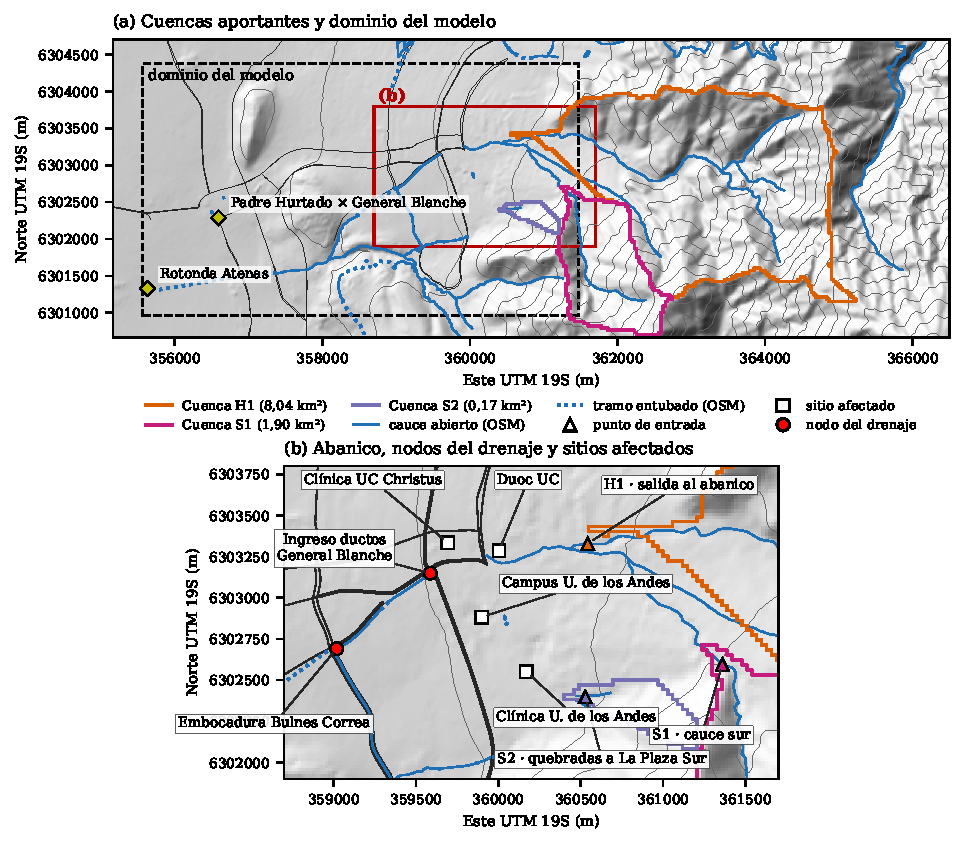
\includegraphics[width=\textwidth]{ubicacion}\caption{Área de estudio. (a) Cuencas aportantes delimitadas sobre el terreno (H1: cauce principal; S1: cauce sur; S2: quebradas menores hacia La Plaza Sur), cauces abiertos y tramos entubados según OpenStreetMap, dominio del modelo y puntos de referencia aguas abajo. (b) Acercamiento al abanico: puntos de entrada del flujo, nodos del drenaje (ingreso a los ductos de General Blanche y embocadura de Francisco Bulnes Correa) y sitios con afectación informada por las fuentes recogidas en la sección~\ref{sec:evidencia}. Coordenadas UTM huso 19 sur, WGS 84.}\label{fig:ubicacion}\end{figure}
\subsection{Evidencia y registro probatorio}\label{sec:evidencia}
Toda consulta a fuentes externas se archivó en un registro probatorio: fecha y hora UTC, origen, dato extraído, captura de la página y huella SHA-256. Este registro deja constancia de la información disponible al modelar y permite contrastar la predicción con observaciones posteriores. Las observaciones se clasificaron según su naturaleza física, como se recomendó en la revisión técnica (véase la declaración final sobre el uso de herramientas de IA):
\begin{itemize}
\item \textbf{Presencia informada:} calles por donde la prensa informa que «bajó» el flujo: Camino El Alba, General Blanche y Quebrada Honda \citep{latercera2026}; además Av.\ La Plaza, donde T13 difundió registros de arrastre de vehículos \citep{t13_2026vehiculos}.
\item \textbf{Cierres municipales:} Mons.\ Álvaro del Portillo y Av.\ San Carlos de Apoquindo \citep{eldinamo2026}. Pueden obedecer a prevención o limpieza.
\item \textbf{Perímetro operativo municipal:} Camino El Alba por el norte, La Plaza por el oriente, Quebrada Honda por el sur y Padre Hurtado por el poniente \citep{latercera2026}. Puede incluir zonas secas.
\item \textbf{Alcance:} hasta el sector del Pueblito Los Dominicos y la Av.\ Padre Hurtado \citep{latercera2026}.
\item \textbf{Sitios con presencia informada por las fuentes:} la urgencia de la Clínica UC Christus, con cerca de \SI{1}{m} de barro \citep{cadena3_2026}; la Clínica Universidad de los Andes, en sus accesos y exterior según la propia clínica \citep{radiolasenal2026}; la sede Duoc UC \citep{biobio2026duoc}; y el campus de la Universidad de los Andes, cuya comunidad quedó retenida \citep{cooperativa2026}. El Servicio Nacional de Prevención y Respuesta ante Desastres (Senapred) incluye la Av.\ La Plaza Sur entre las zonas afectadas \citep{eldinamo2026}.
\item \textbf{Evidencia de baja confiabilidad, usada solo para formular hipótesis:} una imagen difundida en redes sociales que marca varios focos de alimentación del flujo, coherentes con los cauces cartografiados.
\end{itemize}
La lluvia proviene de la estación automática 330019 (Eulogio Sánchez, Tobalaba) de la Dirección Meteorológica de Chile \citeyearpar{dmc2026}: \SI{34,8}{mm} el 8 de octubre, \SI{13,8}{mm} entre las 15:00 y las 21:00 hora local, y, entre el 6 y el 7 de octubre, reportes de \SI{6}{h} que suman \SI{131,2}{mm}, con un máximo de \SI{49,2}{mm} en \SI{6}{h} (una versión anterior de este texto atribuyó por error esos \SI{49,2}{mm} a los dos días). Búsquedas en prensa devolvieron cifras de \SI{16}{mm} a \SI{20}{mm} en alrededor de una hora, sin estación identificada.

\paragraph{Antecedentes hidrometeorológicos conocidos después del cribado.} La alcaldesa informó \SI{144}{mm} acumulados en la zona, \SI{20}{mm} de ellos el día del evento, con suelo saturado \citep{interferencia2026}. El análisis del Centro de Ciencia del Clima y la Resiliencia \citep{cr2_2026} registra en la estación Río Molina \SI{42,8}{mm} el 8 de octubre, \SI{31,6}{mm} entre las 15:00 y las 19:00 y un máximo de \SI{10,9}{mm} en \SI{30}{min}, con la isoterma de \SI{0}{\celsius} cerca de \SI{2800}{m} según el observatorio de Cerro Tres Puntas. El mismo análisis delimita la cuenca entre \SI{929}{m} y \SI{2355}{m} (unos \SI{10,6}{km^2}) y estima la severidad del incendio con el índice normalizado de área quemada diferencial (dNBR) de Sentinel-2. El pronóstico histórico horario de Open-Meteo \citep{openmeteo2023} sitúa la isoterma entre \SI{2700}{m} y \SI{2770}{m} entre las 14:00 y las 17:00 del 8 de octubre, y acumula unos \SI{150}{mm} sobre la cuenca entre el 2 y el 8 de octubre. Las imágenes Sentinel-2 \citep{drusch2012} del 21 de septiembre no muestran nieve en la cuenca (índice normalizado de nieve menor a 0,4 en toda la parte despejada; las zonas blancas eran nubes delgadas), y el análisis de este estudio de las del 9 de octubre estima \SI{0,09}{km^2} de nieve nueva, toda sobre \SI{2000}{m}. La alta cordillera sí tenía un manto abundante: Valle Nevado informó cerca de \SI{1,2}{m} de nieve nueva el 6 y el 7 de octubre \citep{emol2026valle}, por sobre los \SI{3000}{m}.

\paragraph{Contraste con el análisis del CR2.} La tabla~\ref{tab:cr2} compara los datos de cuenca y de forzamiento de este estudio con los del análisis del CR2 \citep{cr2_2026}, publicado después de formular las hipótesis.
\begin{table}[htbp]\centering\small
\caption{Comparación de los datos de cuenca y forzamiento con el análisis del Centro de Ciencia del Clima y la Resiliencia (CR2) \citep{cr2_2026}. La diferencia de área y de cota mínima se debe al punto de cierre: el CR2 cierra la cuenca más abajo, en el parque lineal; este estudio, donde cada cauce entra a la urbanización.}\label{tab:cr2}
\begin{tabular}{p{0.24\textwidth}p{0.3\textwidth}p{0.36\textwidth}}\toprule
Variable & CR2 & Este estudio (datos y estimaciones)\\\midrule
Cota máxima de la cuenca & \SI{2355}{m} & \SI{2355}{m} (FABDEM y Copernicus GLO-30)\\
Cota mínima & \SI{929}{m} & \SI{973}{m} a \SI{1081}{m} (salidas H1, S1, S2)\\
Área & \SI{10,6}{km^2} & \SI{10,1}{km^2}\\
Isoterma de \SI{0}{\celsius} & $\sim\SI{2800}{m}$ (Cerro Tres Puntas) & \SIrange{2700}{2770}{m} entre las 14:00 y las 17:00 (Open-Meteo)\\
Lluvia del 8 de octubre & \SI{42,8}{mm} en Río Molina & mismo dato\\
Incendio & dNBR de Sentinel-2 según el CR2 & dNBR (23-dic-2025 y 6-feb-2026): \SI{82}{\percent} con señal de quema y \SI{10}{\percent} de severidad moderada-alta/alta; usado en el balance y en Gartner (sección~\ref{sec:res-incendio})\\
\bottomrule\end{tabular}
\end{table}

\paragraph{Balances posteriores.} Según La Tercera, Senapred actualizó su balance a 56 viviendas destruidas, 40 con daño mayor, 1.960 con daño menor, 384 personas damnificadas y más de 1.200 rescatadas \citep{latercera2026senapred}.

\subsection{Terreno, edificios y calles}\label{sec:terreno}
\emph{Esta sección describe el terreno de la primera generación (1.103 edificios); la versión con la ciudad completa (42.018 huellas de Overture Maps, cauces tallados según la red hidrográfica oficial y unos 852.000 triángulos) se describe en la sección~\ref{sec:res-v4}.} El terreno sin edificios ni vegetación, es decir, el modelo digital del terreno (DTM), es FABDEM V1-2 \citep{hawker2022,fabdem2023}, con resolución de 1 segundo de arco (unos \SI{30}{m}), remuestreado de forma bilineal a una retícula regular de \SI{4}{m} en el sistema UTM, huso 19 sur (datum WGS~84). El remuestreo aumenta la densidad de puntos, pero no mejora la resolución efectiva del modelo de elevación. Esta limitación debe considerarse al interpretar los resultados. Se incorporaron \num{1107} plantas de edificios de OpenStreetMap (OSM; \citealp{osm2026}) como bloques elevados. La altura de cada bloque es la media de $\mathrm{DSM}-\mathrm{DTM}$, donde el modelo digital de superficie (DSM) es Copernicus GLO-30 \citep{copernicus_glo30} y el DTM es FABDEM, cuando la planta mide al menos \SI{900}{m^2} y la diferencia supera \SI{2,5}{m}. Si no se cumple, la altura es el número de pisos de OSM multiplicado por \SI{3}{m}; sin ese dato, se asumen \SI{6}{m}. Para cada bloque se informan la media y el percentil 95 de $\mathrm{DSM}-\mathrm{DTM}$. Se excluyeron cuatro polígonos de OSM etiquetados como edificio que corresponden a recintos (complejos deportivos y un centro comercial con $\mathrm{DSM}-\mathrm{DTM}$ medio inferior a \SI{4}{m}), porque, representados como bloques sólidos en el modelo, habrían desviado artificialmente el flujo. Las calles se rebajaron \SI{0,15}{m}, altura supuesta del cordón, con un ancho según su categoría.

\subsection{Modelo de propagación}\label{sec:modelo}
Se usa ANUGA, versión 4.0.1 \citep{anuga}: volúmenes finitos sobre una malla triangular no estructurada, con el esquema DE1 (Runge--Kutta de segundo orden). Para una mezcla homogénea de densidad constante, ANUGA resuelve la evolución del caudal unitario $\mathbf q=h\mathbf u$ mediante las ecuaciones de conservación de la masa~\eqref{eq:masa} y de la cantidad de movimiento~\eqref{eq:movimiento}:
\begin{align}
\partial_t h+\nabla\cdot\mathbf q&=S_h,\label{eq:masa}\\
\partial_t\mathbf q+\nabla\cdot\left(\frac{\mathbf q\otimes\mathbf q}{h}+\tfrac12 gh^2\mathbf I\right)&=-gh\nabla z-\frac{\boldsymbol\tau_b}{\rho_m}+S_h\mathbf u_\mathrm{in},\label{eq:movimiento}
\end{align}
donde $h$ es el espesor del flujo (\si{m}); $\mathbf u$, la velocidad media en profundidad (\si{m.s^{-1}}); $\mathbf q=h\mathbf u$, el caudal por unidad de ancho (\si{m^2.s^{-1}}); $z$, la elevación del lecho (\si{m}); $g$, la aceleración de gravedad (\si{m.s^{-2}}); $S_h$, la tasa de aporte de espesor (\si{m.s^{-1}}); $\mathbf u_\mathrm{in}$, la velocidad del aporte (\si{m.s^{-1}}); $\boldsymbol\tau_b$, el esfuerzo de corte basal (\si{Pa}); $\rho_m$, la densidad de la mezcla (\si{kg.m^{-3}}); y $\mathbf I$, el tensor identidad. Al dividir por $\rho_m$, constante, no aparece ningún factor de densidad en la presión ni en la gravedad. La resistencia basal es $\boldsymbol\tau_b/\rho_m=ghS_f\,\mathbf u/U$, con $U=|\mathbf u|$ y la pendiente de fricción $S_f$ dada por
\begin{equation}
S_f=\frac{\tau_y}{\rho_m g h}+\frac{K\eta U}{8\rho_m g h^2}+\frac{n_\mathrm{td}^2U^2}{h^{4/3}},\label{eq:friccion}
\end{equation}
donde $\tau_y$ es el esfuerzo de fluencia (\si{Pa}); $\eta$, la viscosidad dinámica de la mezcla (\si{Pa.s}); $K$, el parámetro adimensional de resistencia laminar; y $n_\mathrm{td}$, el coeficiente de Manning equivalente para la turbulencia y la dispersión (\si{s.m^{-1/3}}). El esfuerzo de fluencia y la viscosidad se obtienen de las relaciones reológicas
\begin{equation}
\tau_y=0{,}1\,\alpha_2e^{\beta_2\Cvf},\qquad \eta=0{,}1\,\alpha_1e^{\beta_1\Cvf},\label{eq:reologia}
\end{equation}
donde $\Cvf$ es la concentración volumétrica de la matriz fina; la densidad $\rho_m$ usa, en cambio, la concentración total $\Cvt$ (sección~\ref{sec:marco}). En las simulaciones del barrido se adopta $\Cvt=\Cvf$. Los coeficientes $(\alpha_1,\beta_1,\alpha_2,\beta_2)$ provienen de la tabla~13 de \citet{flo2d2021}, donde $\alpha_1$ se expresa en poises y $\alpha_2$ en \si{dyn.cm^{-2}}; $\beta_1$ y $\beta_2$ son adimensionales. El factor 0,1 de~\eqref{eq:reologia} convierte ambas magnitudes al SI, de modo que $\tau_y$ resulta en \si{Pa} y $\eta$ en \si{Pa.s}. La muestra Glenwood~2 aparece con tres variantes en distintas versiones de la documentación y se trató como sensibilidad. $K$ y $n_\mathrm{td}$ cambian según la superficie: en calles pavimentadas $K=100$ y $n_\mathrm{td}=0{,}025$; en el resto, $K=400$ y $n_\mathrm{td}=0{,}050$.

La resistencia~\eqref{eq:friccion} se aplica como paso fraccionado y se resuelve de forma implícita en cada celda. Con $a=\tau_y/(\rho_m h)$, $b=K\eta/(8\rho_m h^2)$, $c=gn_\mathrm{td}^2/h^{4/3}$ y $r=(U^*-\Delta t\,a)_+$, se obtiene
\begin{equation}
U^{n+1}=\frac{2r}{1+b\Delta t+\sqrt{(1+b\Delta t)^2+4c\Delta t\,r}},\label{eq:resistencia}
\end{equation}
donde el asterisco indica el estado anterior al paso de resistencia; el superíndice $n+1$, el estado posterior a ese paso; $\Delta t$ es el paso temporal y $(x)_+=\max(x,0)$. La solución~\eqref{eq:resistencia} cumple $0\le U^{n+1}\le U^*$, conserva la dirección, disipa energía y no modifica $h$. Si $|\mathbf q^*|\le\Delta t\,\tau_y/\rho_m$, la celda se detiene y puede reactivarse en pasos posteriores. La fricción de Manning propia de ANUGA se anula para no duplicar la resistencia.

La mezcla entra mediante un hidrograma triangular de caudal pico $Q_p$, volumen de mezcla $V_m$ y tiempo al pico de \SI{600}{s}, con base $T_B=2V_m/Q_p$. Cada fuente agrega en un círculo de \SI{14}{m} de radio el incremento de espesor $\Delta h$ correspondiente al volumen aportado por el hidrograma durante el paso, junto con su momento: $h^+=h^-+\Delta h$ y $\mathbf q^+=\mathbf q^-+\Delta h\,\mathbf u_\mathrm{in}$, donde los superíndices $-$ y $+$ indican los estados anterior y posterior al aporte, y $\mathbf u_\mathrm{in}$ se orienta según el eje del cauce. Cuando $Q=0$ no hay forzamiento. En H3, cada fuente recibe la fracción del hidrograma correspondiente al área de su cuenca. La malla de la primera generación tiene unos \num{4,3e5} triángulos: \SI{40}{m^2} en el corredor entre los cauces y Padre Hurtado (lado equivalente de unos \SI{10}{m}) y \SI{600}{m^2} fuera de él. La aceleración de gravedad es $g=\SI{9,8}{m.s^{-2}}$ en todo el modelo. En la primera generación, las simulaciones duran $T_B+\SI{1200}{s}$ y en cada una se registra el balance de volumen. Las variantes de ciudad, lluvia medida y malla fina del campus se describen en las secciones~\ref{sec:res-v4} y~\ref{sec:res-posterior}.

\begin{table}[htbp]\centering\small
\caption{Parámetros físicos y numéricos aplicados en las simulaciones. Los coeficientes reológicos son los de la tabla de muestras de O'Brien y Julien recopilada en el manual de FLO-2D \citep{flo2d2021}; $\tau_y=0{,}1\,\alpha_2e^{\beta_2C_v}$ en Pa y $\eta=0{,}1\,\alpha_1e^{\beta_1C_v}$ en Pa\,s.}\label{tab:parametros}
\begin{adjustbox}{max width=\textwidth}\begin{tabular}{lrrrrrrr}\toprule
Muestra & $\alpha_1$ & $\beta_1$ & $\alpha_2$ & $\beta_2$ & \multicolumn{3}{c}{$\tau_y$ (Pa) / $\eta$ (Pa\,s) con $C_v=$}\\\cmidrule(l){6-8}
 & & & & & 0,35 & 0,40 & 0,45\\\midrule
Glenwood 1 & 0{,}0028 & 23{,}00 & 0{,}0345 & 20{,}10 & 3{,}9 / 0{,}89 & 10{,}7 / 2{,}80 & 29{,}2 / 8{,}85\\
Glenwood 2a & 0{,}0648 & 6{,}20 & 0{,}0765 & 16{,}90 & 2{,}8 / 0{,}06 & 6{,}6 / 0{,}08 & 15{,}4 / 0{,}11\\
Glenwood 2b & 0{,}6480 & 6{,}20 & 0{,}0765 & 16{,}90 & 2{,}8 / 0{,}57 & 6{,}6 / 0{,}77 & 15{,}4 / 1{,}06\\
Glenwood 2c & 0{,}6480 & 8{,}20 & 0{,}0765 & 16{,}90 & 2{,}8 / 1{,}14 & 6{,}6 / 1{,}72 & 15{,}4 / 2{,}59\\
Aspen 1 & 0{,}0360 & 22{,}10 & 0{,}1810 & 25{,}70 & 145{,}9 / 8{,}23 & 527{,}5 / 24{,}86 & 1906{,}8 / 75{,}05\\
Aspen 2 & 0{,}0538 & 14{,}50 & 2{,}7200 & 10{,}40 & 10{,}4 / 0{,}86 & 17{,}4 / 1{,}78 & 29{,}3 / 3{,}67\\
\midrule
\multicolumn{8}{l}{\textbf{Mezcla y constantes}}\\
\multicolumn{5}{l}{Densidad del agua $\rho_w$ / de los sólidos $\rho_s$} & \multicolumn{3}{r}{\SI{1000}{kg/m^3} / \SI{2650}{kg/m^3}}\\
\multicolumn{5}{l}{Densidad de la mezcla $\rho_m=\rho_w+C_v(\rho_s-\rho_w)$, $C_v=0{,}35/0{,}40/0{,}45$} & \multicolumn{3}{r}{1578 / 1660 / 1742 kg/m$^3$}\\
\multicolumn{5}{l}{Gravedad $g$} & \multicolumn{3}{r}{\SI{9,8}{m/s^2}}\\
\multicolumn{5}{l}{Resistencia laminar $K$ (calles / resto)} & \multicolumn{3}{r}{100 / 400}\\
\multicolumn{5}{l}{Manning turbulento-dispersivo $n_{td}$ (calles / resto)} & \multicolumn{3}{r}{0,025 / 0,050 s\,m$^{-1/3}$}\\
\multicolumn{8}{l}{\textbf{Entrada, malla y cálculo}}\\
\multicolumn{5}{l}{Volumen de mezcla $V$ / caudal pico $Q_p$ / tiempo al pico $t_p$} & \multicolumn{3}{r}{80--300 mil m$^3$ / 100--250 m$^3$/s / 600 s}\\
\multicolumn{5}{l}{Velocidad de entrada / radio de cada fuente} & \multicolumn{3}{r}{2 m/s / 14 m}\\
\multicolumn{5}{l}{Área máxima de triángulo (corredor / resto); triángulos, primera generación} & \multicolumn{3}{r}{40 / 600 m$^2$; $\approx$430\,000}\\
\multicolumn{5}{l}{Grilla del terreno; rebaje de calles; altura supuesta de edificios} & \multicolumn{3}{r}{4 m; 0,15 m; 6 m}\\
\multicolumn{5}{l}{Número de Courant (cribado / lluvia / final)} & \multicolumn{3}{r}{1 / 0,5 / $\le$0,25}\\
\multicolumn{5}{l}{Umbral de mojado para la evaluación $h^*$} & \multicolumn{3}{r}{5 cm (sensibilidad 2 y 10 cm)}\\
\bottomrule\end{tabular}\end{adjustbox}\end{table}

\begin{figure}[htbp]\centering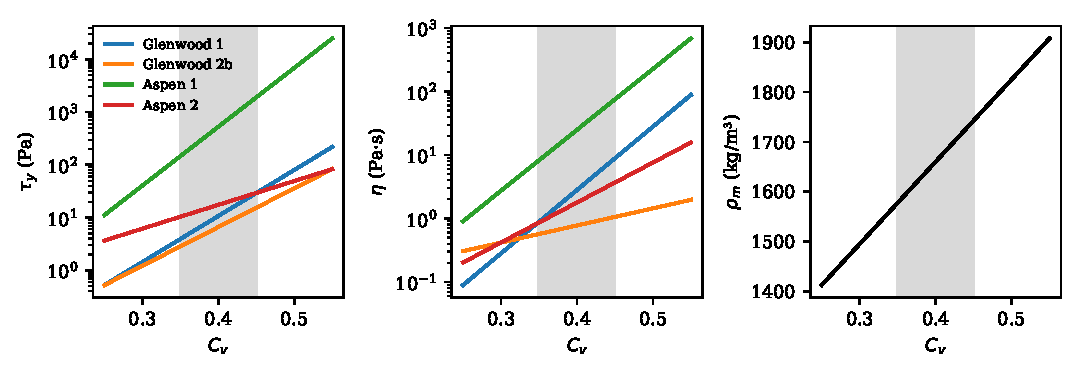
\includegraphics[width=\textwidth]{reologia}\caption{Propiedades calculadas de la mezcla según la concentración volumétrica de sólidos $C_v$ para las muestras ensayadas: esfuerzo de fluencia $\tau_y$, viscosidad $\eta$ y densidad $\rho_m$. La franja gris indica el rango inicial (0,35--0,45); los ensayos posteriores amplían las concentraciones (sección~\ref{sec:res-posterior}).}\label{fig:reologia}\end{figure}

\subsection{Verificación numérica}\label{sec:verif}
\paragraph{Parada.} Sobre un plano de pendiente $S_0=0{,}05$, con $\tau_y=\SI{100}{Pa}$ y $\rho_m=\SI{1700}{kg.m^{-3}}$, la teoría de un fluido de Bingham integrado en la profundidad predice un espesor de reposo $h_c=\tau_y/(\rho_m gS_0)=\SI{0,1200}{m}$. Se libera un bloque de mezcla y se compara el espesor simulado del depósito con el espesor teórico de reposo; se verifica además que el momento se anule.

\paragraph{Reinicio.} A partir del depósito detenido se agrega mezcla aguas arriba y se verifica que el depósito se reactive, vuelva a detenerse y conserve el volumen.

\paragraph{Convergencia temporal.} El ensayo de parada se repite con números de Courant--Friedrichs--Lewy (CFL) de 1; 0,5; 0,25; 0,1 y 0,05 con el esquema DE1, y con el esquema DE0 como comparación; se compara el alcance final del frente y se estima el orden de convergencia respecto del límite extrapolado.

\paragraph{Balance de volumen.} En cada simulación se compara el volumen acumulado aportado por el hidrograma con el volumen presente en la malla.

Los resultados de estas pruebas se presentan en la sección~\ref{sec:res-verif}.

\subsection{Volumen previo independiente}\label{sec:volumen}
Las cuencas se delimitaron con direcciones de flujo calculadas por el método de ocho direcciones (D8) sobre FABDEM reproyectado al sistema UTM, huso 19 sur (datum WGS~84), con celdas de \SI{30}{m}. Una delimitación preliminar en coordenadas geográficas subestimaba el área. La salida de cada cuenca es la celda de máxima acumulación a menos de \SI{120}{m} del punto donde el cauce cartografiado entra a la urbanización. Resultan H1 con \SI{8,04}{km^2} y un relieve de \SI{1376}{m}, S1 con \SI{1,90}{km^2} y S2 con \SI{0,17}{km^2}: en total, \SI{10,1}{km^2} aportantes.

Se usaron dos estimaciones independientes, que no se combinan en una sola distribución:
\begin{itemize}
\item \textbf{Balance lluvia--escorrentía con agua y sólidos diferenciados:} $V_w=f_wPAC$ y $V_m=V_w/(1-\Cvt)$, donde $V_w$ es el volumen de agua incorporado al pulso; $P$, la precipitación acumulada; $A$, el área de la cuenca; $C$, el coeficiente de escorrentía; $f_w$, la fracción de escorrentía incorporada al pulso; y $V_m$, el volumen de mezcla. Los rangos son: precipitación del pulso del evento $P$ entre \SI{12}{\milli\metre} y \SI{35}{\milli\metre}, $C\in[0{,}3;0{,}8]$, $f_w\in[0{,}5;1]$ y $\Cvt\in[0{,}30;0{,}50]$.
\item \textbf{Modelo empírico para cuencas quemadas} \citep{gartner2014}, aplicado por subcuenca e incluyendo su error residual $\varepsilon\sim N(0;1{,}04^2)$. Ese modelo predice el volumen de depósito $V_\mathrm{dep}$, que se convierte a volumen de mezcla con $V_m=(1-\phi)V_\mathrm{dep}/\Cvt$, donde $\phi$ es la porosidad del depósito. Su aplicabilidad fuera del sur de California es una hipótesis.
\end{itemize}
Las distribuciones se resumen mediante la mediana y los percentiles 5 y 95, y el caudal pico correspondiente se estima con la relación de \citet{mizuyama1992}. La calibración recorre volúmenes de \SI{80000}{\metre\cubed} a \SI{300000}{\metre\cubed}. Los resultados iniciales se presentan en la sección~\ref{sec:res-volumen}; la actualización con severidad estimada por dNBR, en la sección~\ref{sec:res-incendio}.

\begin{figure}[htbp]\centering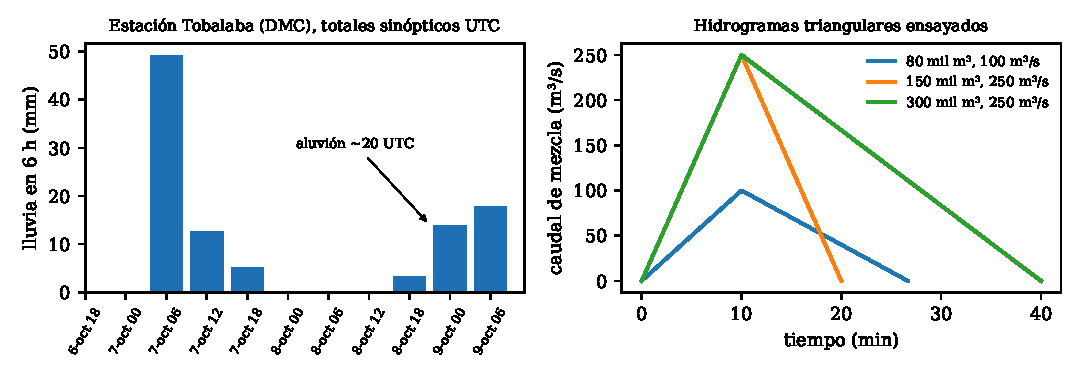
\includegraphics[width=\textwidth]{forzamiento}\caption{Forzamiento observado y supuesto del modelo. Izquierda: lluvia acumulada cada \SI{6}{h} en la estación Tobalaba de la Dirección Meteorológica de Chile \citep{dmc2026} entre el 6 y el 9 de octubre de 2026 (horas UTC; la prensa citada en el relato sitúa el aluvión hacia las 20 UTC del 8 de octubre). Derecha: hidrogramas triangulares de mezcla ensayados.}\label{fig:forzamiento}\end{figure}

\paragraph{Escenario de suelo saturado.} Con la información hidrometeorológica conocida después del cribado (sección~\ref{sec:evidencia}) se agregó una tercera estimación, tampoco combinada con las anteriores. La relación entre la isoterma informada y la cota máxima de la cuenca (\SI{2355}{m}, igual a la que informa el CR2; una versión previa del texto indicó por error \SI{2775}{m}, cifra que no se usó en ningún cálculo: la delimitación D8 y la hipsometría siempre se basaron en la cota del modelo de elevación) sustenta el supuesto de precipitación líquida sobre toda el área aportante, y la saturación del suelo informada por la autoridad se adopta como supuesto del escenario de cálculo. Se usan $P\in[20;40]$~\si{mm}, $C\in[0{,}6;0{,}9]$ y $f_w\in[0{,}6;1]$. El aporte por fusión de nieve se acota por arriba con \SI{50}{mm} de equivalente en agua sobre los \SI{0,31}{km^2} de la cuenca situados sobre \SI{2000}{m}.

\subsection{Calibración inversa e incertidumbre}\label{sec:calib}
La calibración sigue el enfoque de simulaciones de comportamiento aceptable \citep{beven1992}. Los criterios se fijaron antes de examinar los resultados:
\begin{enumerate}
\item fracción $R$ de puntos sobre calles con presencia informada por las fuentes en que $h_\mathrm{max}>h^*$, con $R\ge0{,}6$;
\item fracción $R_\mathrm{sit}$ de los cuatro sitios con presencia informada por las fuentes que el flujo alcanza dentro de \SI{40}{m}, con $R_\mathrm{sit}\ge3/4$;
\item llegada a menos de \SI{200}{m} del cruce de General Blanche con Padre Hurtado;
\item fracción $F_\mathrm{per}$ del área afectada que cae dentro del perímetro municipal ampliado en \SI{100}{m}, con $F_\mathrm{per}\ge0{,}5$. Desde el 11 de octubre, cuando se publicó la zona afectada oficial \citep{bbnn2026visor}, $F_\mathrm{per}$ se calcula con ese polígono y solo sobre el barro simulado en zona urbana (a menos de \SI{40}{m} de un edificio), para no contar los cerros mojados por la lluvia.
\end{enumerate}
El umbral es $h^*=\SI{5}{cm}$, con sensibilidad para \SI{2}{cm} y \SI{10}{cm}. Cada simulación aceptable recibe un peso informal $L=R\,R_\mathrm{sit}\,F_\mathrm{per}$. Las calles cerradas por el municipio se usan solo como contexto, porque un cierre puede ser preventivo. El índice de Jaccard respecto del perímetro se informa como dato descriptivo, ya que el perímetro es operativo y no una huella cartografiada.

El barrido recorre las hipótesis H1, H2 y H3; volúmenes de mezcla de \SI{80000}{\metre\cubed}, \SI{150000}{\metre\cubed} y \SI{300000}{\metre\cubed}; caudales pico de \SI{100}{\metre\cubed\per\second} y \SI{250}{\metre\cubed\per\second}; y tres muestras reológicas (Glenwood~1, Glenwood~2b y Aspen~2). El cribado usó CFL~1. Se completaron controles con paso temporal fino (z01, z02, z26, z29 y z32) y el ensayo con malla fina en el campus (m36), según las secciones~\ref{sec:res-verif} y~\ref{sec:res-posterior}.

\subsection{Síntesis del conjunto e indicadores por calle y edificio}\label{sec:sintesis}
\paragraph{Tres niveles de evaluación.} Se distinguen: (i) los \emph{criterios de aceptación originales}, fijados antes de simular con un umbral para cada uno (sección~\ref{sec:calib}); con el terreno anterior ninguna simulación los cumplía todos; la candidata a la prueba reservada (z02) cumple tres de cuatro (no cumple el de perímetro), mientras que los ajustes posteriores de casas porosas (z26) y de la hipótesis integrada con lluvia supuesta (z32) cumplen los cuatro; (ii) el \emph{índice exploratorio de compatibilidad} (IEC), definido después, que resume los mismos cuatro criterios en una escala continua para comparar hipótesis; y (iii) la \emph{validación independiente} de los ajustes posteriores, no probada al cierre, que exige datos no usados para formular las hipótesis, como imágenes satelitales posteriores al evento, levantamientos oficiales de depósitos o marcas de nivel.

\paragraph{Índice exploratorio de compatibilidad.} Para comparar hipótesis se resume cada simulación en un \emph{índice exploratorio de compatibilidad} (IEC) con lo observado, en una escala de 0 a 100: el promedio de cuatro componentes, cada uno entre 0 y 1, derivados de los criterios originales fijados antes de simular (sección~\ref{sec:calib}); el índice se definió después y la referencia de perímetro se actualizó con el polígono oficial. Son la fracción de puntos de las calles con barro informado por las fuentes que el modelo moja ($R$); la fracción de los cuatro recintos con afectación informada alcanzados ($R_\mathrm{sit}$); el alcance, igual a 1 si el barro llega a menos de \SI{200}{m} de Padre Hurtado y decreciente en forma lineal hasta 0 a \SI{1200}{m}; y $F_\mathrm{per}$. El IEC no es una probabilidad ni una medida de precisión predictiva: resume qué tan bien una simulación reproduce un conjunto de observaciones cualitativas, y diferencias de dos o tres puntos no deben interpretarse como evidencia concluyente de superioridad entre hipótesis. Las profundidades, velocidades y presiones por calle y edificio se extraen como el máximo en un radio de \SI{40}{m} de cada punto de interés.


\section{Datos de entrada y funcionamiento del modelo: guía para aplicarlo a otras cuencas}\label{sec:transferencia}
Esta sección describe el método en términos generales, sin referencia a productos ni programas concretos, para que pueda aplicarse a otras cuencas con los datos que cada caso tenga disponibles. Se indica qué representa cada dato, la calidad mínima recomendable, cómo entra en el cálculo y cómo afecta al resultado cuando es incierto.

\subsection*{Cómo funciona el modelo}
El modelo resuelve, en cada instante y en cada celda de una malla que cubre la ciudad, cuánto barro hay (espesor) y hacia dónde y a qué velocidad se mueve. Lo hace con tres principios:
\begin{enumerate}
\item \textbf{Conservación de la masa:} el barro que entra a una celda y no sale se acumula como espesor. No se crea ni se pierde barro; el balance se verifica en cada simulación.
\item \textbf{Conservación del momento:} el barro acelera pendiente abajo por la gravedad, según la inclinación de la superficie libre y no solo la del suelo, y lo frenan la resistencia del propio material y el roce con la superficie. Por eso puede subir sobre una solera si llega con velocidad, rodear un edificio o embalsarse detrás de un obstáculo.
\item \textbf{Comportamiento del material:} a diferencia del agua, una mezcla densa de agua y sedimento tiene un \emph{umbral de fluencia}: si el empuje de la gravedad sobre una capa no lo supera, la capa se detiene. Por eso el barro deja depósitos de cierto espesor en lugar de escurrir hasta la cota más baja. Sobre ese umbral, la mezcla se comporta como un fluido muy viscoso y turbulento.
\end{enumerate}
La simulación avanza en pasos de tiempo cortos, de fracciones de segundo, limitados por la velocidad del flujo y el tamaño de las celdas. En cada paso se calculan primero el transporte y la gravedad, y después el frenado del material, que puede detener una celda o reactivarla si llega más barro desde aguas arriba. Durante la simulación se registran, para cada celda, el espesor máximo, la velocidad máxima, el empuje dinámico sobre obstáculos y el instante de llegada del frente.

\subsection*{Datos de entrada}
\begin{table}[htbp]\centering\small
\caption{Datos de entrada para aplicar el modelo a otras cuencas: significado, calidad recomendable y efecto de la incertidumbre sobre los resultados calculados.}\label{tab:transferencia}
\begin{tabular}{p{0.17\textwidth}p{0.25\textwidth}p{0.22\textwidth}p{0.245\textwidth}}\toprule
Dato & Qué representa y cómo se usa & Calidad recomendable & Efecto si es incierto\\\midrule
Relieve del terreno desnudo & Cotas del suelo sin edificios ni árboles; define pendientes y hacia dónde escurre el flujo. & Preferentemente \SIrange{1}{5}{m} de resolución; \SI{30}{m} solo reproduce la dirección general. & Es el dato más influyente: un cauce o una calle que el relieve no resuelve cambia el recorrido.\\
Huellas y alturas de edificios & Obstáculos que el flujo rodea; se elevan sobre el terreno. & Huellas completas; altura por levantamiento o número de pisos. & Desvían el flujo localmente; poca influencia en el recorrido general si las huellas representan adecuadamente la geometría de los edificios.\\
Calles y soleras & Corredores preferentes; se rebajan unos centímetros respecto de las veredas. & Eje y ancho de cada calle; cota de solera si existe. & Determinan qué calles actúan como canales.\\
Cauces abiertos y tramos entubados & Dónde la quebrada va por superficie y dónde bajo tierra; los puntos de transición son candidatos a desborde. & Trazado, sección y capacidad de cada tramo. & Si falta un cauce abierto, el modelo lo sustituye por la pendiente general; si falta un ducto, no se puede evaluar su desborde.\\
Cuenca aportante & Área y relieve que drenan a cada punto de entrada a la ciudad; se obtienen del relieve. & Relieve de la cuenca alta; \SI{30}{m} suele bastar. & Escala el volumen esperado en proporción al área.\\
Lluvia & Cantidad e intensidad del episodio y de los días previos (humedad del suelo). & Estación cercana con registro horario o subhorario; preferentemente en la cuenca alta. & Con la cuenca, acota el volumen; la intensidad de corta duración controla el caudal pico.\\
Estado de la cuenca & Superficie quemada, cobertura vegetal, suelo. & Cartografía de severidad del incendio. & Condiciona los coeficientes supuestos de escorrentía y carga de sedimento.\\
Volumen e hidrograma & Cuánta mezcla entra, con qué caudal máximo y en cuánto tiempo. & Estimados a partir de lluvia y cuenca, de relaciones empíricas o de depósitos medidos tras el evento. & Controlan el alcance y las profundidades; se acotan mediante calibración.\\
Propiedades del material & Densidad, umbral de fluencia y viscosidad de la mezcla, según la concentración de sólidos. & Ensayos de muestras del depósito; si no los hay, rangos de la literatura. & Controlan cuándo y dónde se detiene el flujo.\\
Observaciones del evento & Calles y edificios afectados, alcance, profundidades, horas. & Puntos georreferenciados con fuente y hora; marcas de nivel. & No alimentan el modelo: permiten descartar hipótesis y calibrar.\\
\bottomrule\end{tabular}\end{table}

\subsection*{Procedimiento para otra cuenca}
\begin{enumerate}
\item \textbf{Delimitar el área urbana expuesta} y los puntos donde los cauces entran a la ciudad o cambian de abiertos a entubados. Esos puntos son las entradas posibles del flujo.
\item \textbf{Construir la superficie de cálculo:} relieve desnudo, edificios elevados, calles rebajadas y, si es posible, cauces abiertos con su sección real.
\item \textbf{Estimar un rango de volumen} con al menos dos vías independientes (lluvia por cuenca por coeficiente de escorrentía, y relaciones empíricas para cuencas similares), sin combinarlas en una sola cifra.
\item \textbf{Formular hipótesis de entrada} (por qué puntos sale el flujo a la superficie y en qué proporción) y fijar \emph{antes} de simular los criterios con que se juzgará cada una frente a las observaciones.
\item \textbf{Simular cada combinación} de hipótesis, volumen, caudal y material; verificar en cada simulación el balance de masa y la estabilidad numérica.
\item \textbf{Comparar con las observaciones}, conservar las combinaciones compatibles e informar el conjunto como un rango de escenarios y no como una única respuesta.
\item \textbf{Repetir las simulaciones compatibles con mayor resolución temporal y espacial}, para estimar el error numérico de alcances y tiempos.
\end{enumerate}

\subsection*{Qué mejora más el resultado}
En este caso de estudio, el orden de influencia de las incertidumbres fue: el relieve (resolución y representación de cauces y calles), las propiedades del material, el volumen y la forma del hidrograma, y las alturas de los edificios. Un levantamiento de alta resolución del sector urbano y del cauce, y muestras del depósito, son las dos mejoras de mayor rendimiento. Para fines preventivos, sin un evento que calibrar, el método se aplica igual, pero con escenarios de volumen y material elegidos según la cuenca y presentando las envolventes de afectación en lugar de un recorrido único.


\section{Resultados}\label{sec:resultados}
\emph{Resultados al cierre (13 de octubre de 2026): 84 simulaciones completadas, 19 de cribado con el terreno anterior, 41 con la ciudad completa, 5 de cuadratura de la concentración y 19 microsimulaciones del campus. Las secciones~\ref{sec:res-v4} a~\ref{sec:res-campus} usan el terreno con la ciudad completa; la sección~\ref{sec:res-calib} conserva el cribado inicial con el terreno anterior, como referencia del proceso.}

\subsection{Simulaciones con la ciudad completa}\label{sec:res-v4}
La versión del terreno utilizada para los resultados urbanos incorpora las 42.018 huellas de edificios de Overture Maps sobre FABDEM a \SI{4}{m}, amplía el dominio hasta Paul Harris, el Hospital Dipreca y la rotonda Atenas, y talla tres cauces que el modelo de elevación de \SI{30}{m} no resuelve: el parque lineal hasta la embocadura de Francisco Bulnes Correa, Quebrada Honda aguas abajo de la embocadura según la red hidrográfica oficial y el brazo sur hasta la parte alta de la Av.\ Monseñor Álvaro del Portillo. La malla tiene unos 852.000 triángulos. La tabla~\ref{tab:v4} resume las simulaciones; el anexo~\ref{sec:anexo} contiene el catálogo de las corridas de cribado, ciudad y cuadratura y una ficha con lámina por simulación clave.

\begin{table}[htbp]\centering\small
\caption{Simulaciones con la ciudad completa (42.018 edificios). Las capacidades del colector son parámetros supuestos de escenarios hipotéticos; no describen la obra real. Calles: fracción de puntos de las calles con barro informado por las fuentes que el modelo moja ($h>\SI{5}{cm}$); Sitios: fracción de los cuatro recintos con afectación informada alcanzados por el flujo simulado; dPH: distancia mínima del barro simulado al cruce de General Blanche con Padre Hurtado; Perím.: fracción del barro simulado en zona urbana que cae dentro de la zona afectada oficial (IDE Chile); QH: fracción de Quebrada Honda con barro simulado; UCC: espesor máximo calculado junto a la Clínica UC Christus (Cadena 3 informó cerca de \SI{1}{m} en urgencias); IEC: índice exploratorio de compatibilidad, promedio de los cuatro criterios (calles, sitios, alcance y perímetro) en escala de 0 a 100; no es precisión predictiva. Barro: G2b, Glenwood~2b ($C_v=0{,}40$); G1, Glenwood~1 ($C_v=0{,}45$); A2, Aspen~2.}\label{tab:v4}
{\setlength{\tabcolsep}{3.5pt}\begin{adjustbox}{max width=\textwidth}\begin{tabular}{llrlrrrrrrr}\toprule
Corrida & Escenario & $V$ (mil m$^3$) & Barro & Calles & Sitios & dPH (m) & Perím. & QH & UCC (m) & IEC\\
\midrule
z02 & cauce + brazos sur; lluvia 35 mm/h, paso 4× más fino & 300 & G2b & 0{,}77 & 0{,}75 & 15 & 0{,}34 & 0{,}68 & 1{,}13 & 72\\
v02 & cauce + brazos sur; lluvia 35 mm/h en ladera & 300 & G2b & 0{,}77 & 0{,}75 & 15 & 0{,}34 & 0{,}68 & 1{,}13 & 72\\
v19 & cauce + brazos sur; lluvia 35 mm/h + brazo sur oficial hasta Álvaro del Portillo (terreno v6) & 300 & G2b & 0{,}77 & 0{,}75 & 15 & 0{,}34 & 0{,}68 & 1{,}11 & 71\\
v14 & cauce + brazos sur; lluvia 35 mm/h + quebrada Álvaro del Portillo & 300 & G2b & 0{,}77 & 0{,}75 & 15 & 0{,}34 & 0{,}68 & 1{,}15 & 71\\
v01 & cauce principal & 300 & G2b & 0{,}77 & 0{,}50 & 96 & 0{,}46 & 0{,}68 & 1{,}16 & 68\\
z01 & cauce principal; control numérico (paso 4× más fino) & 300 & G2b & 0{,}77 & 0{,}50 & 96 & 0{,}46 & 0{,}68 & 1{,}16 & 68\\
v15 & cauce principal; Quebrada Honda tallada aguas abajo (terreno v5) & 300 & G2b & 0{,}77 & 0{,}50 & 96 & 0{,}45 & 0{,}68 & 1{,}18 & 68\\
v03 & cauce principal; colector con capacidad supuesta de 30 m$^3$/s & 300 & G2b & 0{,}77 & 0{,}50 & 96 & 0{,}50 & 0{,}64 & 1{,}16 & 69\\
v17 & cauce principal; colector con capacidad supuesta de 30 m$^3$/s, captura 25 m, Quebrada Honda tallada & 300 & G2b & 0{,}76 & 0{,}50 & 96 & 0{,}50 & 0{,}62 & 1{,}18 & 69\\
v05 & cauce principal; colector con capacidad supuesta de 100 m$^3$/s & 300 & G2b & 0{,}74 & 0{,}50 & 96 & 0{,}53 & 0{,}44 & 1{,}16 & 69\\
v10 & cauce principal; colector con capacidad supuesta de 100 m$^3$/s, captura 25 m & 300 & G2b & 0{,}69 & 0{,}50 & 96 & 0{,}52 & 0{,}00 & 1{,}16 & 68\\
v18 & cauce principal; colector con capacidad supuesta de 100 m$^3$/s, captura 25 m, Quebrada Honda tallada & 300 & G2b & 0{,}69 & 0{,}50 & 96 & 0{,}52 & 0{,}00 & 1{,}18 & 68\\
v07 & cauce principal & 150 & G2b & 0{,}72 & 0{,}50 & 348 & 0{,}62 & 0{,}68 & 1{,}09 & 67\\
v08 & cauce principal & 300 & G1 & 0{,}74 & 0{,}50 & 396 & 0{,}63 & 0{,}69 & 1{,}16 & 67\\
v09 & cauce principal & 300 & A2 & 0{,}77 & 0{,}50 & 151 & 0{,}52 & 0{,}68 & 1{,}14 & 70\\
v21 & cauce + brazos sur; brazo sur oficial (terreno v6), sin lluvia & 300 & G2b & 0{,}77 & 0{,}50 & 131 & 0{,}45 & 0{,}68 & 1{,}11 & 68\\
\bottomrule\end{tabular}\end{adjustbox}}
\end{table}


Cuatro resultados destacan:
\begin{enumerate}
\item \textbf{La ciudad representada encauza el barro en el modelo.} Con todos los edificios, el espesor calculado en el entorno de la Clínica UC Christus sube de \SI{0,3}{m} a \SIrange{1,1}{1,2}{m}, del orden del metro que Cadena 3 informó en su urgencia (un máximo próximo al recinto no representa necesariamente su interior), y junto a Duoc UC llega a \SI{1,9}{m}. El barro alcanza mayor profundidad en las calles y cubre menos superficie: unas \SI{54}{ha} dentro de la zona afectada oficial, frente a \SI{93}{ha} con el terreno anterior.
\item \textbf{Volumen.} En el modelo, con \SI{150000}{m^3} el frente se detiene a \SI{348}{m} de Padre Hurtado; con \SI{300000}{m^3} llega a menos de \SI{100}{m}. Ese volumen coincide con la estimación independiente con suelo saturado (sección~\ref{sec:res-volumen}).
\item \textbf{Hipótesis seleccionada para la prueba reservada.} El cauce principal más los brazos sur y la lluvia de \SI{35}{mm/h} sobre la ladera (z02, v02) obtiene un IEC de 72/100 (calles 0,77; recintos 0,75; alcance 1,00; zona afectada oficial 0,34): reproduce presencia de flujo en el \SI{77}{\percent} de los puntos de control de las calles consideradas, tres de los cuatro recintos ---incluida la Clínica Universidad de los Andes, con \SI{0,14}{m}--- y el alcance, pero solo un tercio de su barro urbano cae dentro de la zona afectada oficial. Sin la lluvia supuesta en la ladera (v21), el modelo no alcanza la Clínica Universidad de los Andes y el IEC baja a 68/100.
\item \textbf{Robustez.} z02 repite v02 con un paso de tiempo cuatro veces menor y da los mismos indicadores; z01 hace lo mismo con el cauce principal solo. El barro muy fluido (Aspen~2) obtiene 70/100; el espeso (Glenwood~1) se detiene a \SI{396}{m} de Padre Hurtado. El IEC de v20 con paso de tiempo normal (78/100) depende de \SI{10}{cm} en un solo punto del campus y no se repite con paso fino (v19), por lo que no se considera.
\end{enumerate}

\subsection{Capacidad del colector de Francisco Bulnes Correa: escenarios hipotéticos}\label{sec:res-colector}
Esta sección es un análisis de escenarios hipotéticos. No se dispuso de información pública sobre la capacidad, la sección y el estado reales del colector; los valores siguientes no evalúan la obra ni constituyen una conclusión oficial, y requieren validación con información de diseño e inspección. \emph{Resultado calculado:} con la ciudad completa y la hipótesis de volumen adoptada, el caudal de mezcla que llega a la embocadura alcanza unos \SI{65}{m^3/s}, cuatro veces más que con el terreno anterior. \emph{Escenarios hipotéticos:} si el sumidero del modelo capta toda la sección del cauce (radio de captura de \SI{25}{m} a \SI{40}{m}), con capacidad supuesta de \SI{100}{m^3/s} o \SI{200}{m^3/s} retira unos \SI{93000}{m^3} con un pico de \SI{62}{m^3/s} a \SI{66}{m^3/s} y Quebrada Honda queda seca (v10, v11, v18). Con capacidad supuesta de \SI{30}{m^3/s}, el sumidero alcanza ese límite, retira \SI{67600}{m^3} y Quebrada Honda se moja en el \SI{62}{\percent} de sus puntos (v17). En estos escenarios, el intervalo calculado de capacidad supuesta para que no quede flujo superficial aguas abajo del sumidero se sitúa entre \SI{30}{m^3/s} y unos \SI{65}{m^3/s}; ese intervalo depende del volumen, del hidrograma y de la reología supuestos. \emph{Por qué cambió respecto de la primera generación.} Con 1.103 edificios el barro se repartía en superficie y a la embocadura llegaban \SI{12800}{m^3} con un pico de \SI{16,5}{m^3/s}, que el sumidero del modelo con capacidad supuesta de \SI{30}{m^3/s} retira. En el modelo con las 42.018 huellas, las calles concentran el flujo, aumentan la velocidad y entregan a la embocadura unos \SI{93000}{m^3} con un pico cercano a \SI{65}{m^3/s}. Ambos resultados son calculados y dependen de la representación urbana; la versión con la ciudad completa es la vigente. Un radio de captura de \SI{12}{m} dejaba pasar el flujo por el costado del sumidero y producía un \SI{44}{\percent} de Quebrada Honda con barro aun con \SI{100}{m^3/s}; era un artefacto de representación, corregido al captar toda la sección. La cartografía hidrográfica oficial representa la continuidad del cauce desde la embocadura por Quebrada Honda hacia el Hospital Dipreca; en las simulaciones, el flujo que no ingresa al colector continúa por ese trazado.

\subsection{Contraste con la zona afectada oficial}\label{sec:res-oficial}
El visor de emergencia del Ministerio de Bienes Nacionales, desarrollado por IDE Chile, publica la zona afectada (\SI{288,5}{ha}), 2.266 predios y 368 tramos de calles afectadas \citep{bbnn2026visor}. La zona es la franja entre dos corredores: Camino El Alba y General Blanche por el norte, y Quebrada Honda por el sur, con una prolongación por Camino El Alba al poniente de Padre Hurtado (figura~\ref{fig:ide}). El barro simulado corre por esos dos bordes, pero deja seco el interior de la franja y se extiende fuera de ella en tres sectores: los cerros y quebradas mojados por la lluvia en la ladera, la trama al poniente de Padre Hurtado (\SIrange{8}{20}{ha}) y Quebrada Honda aguas abajo hacia Dipreca (\SIrange{14}{26}{ha}), con espesores de \SI{0,3}{m} a \SI{0,4}{m}. Como los predios publicados son el universo del perímetro y no predios con barro verificado (el \SI{91}{\percent} está dentro de la zona), la fracción de predios tocados por el barro simulado (717 de 2.266, \SI{32}{\percent} en z02) sirve para comparar simulaciones, no como tasa de acierto. Con este polígono, el criterio de perímetro baja y el IEC de z02 pasa de 74/100 (perímetro de prensa) a 72/100.

\begin{figure}[htbp]\centering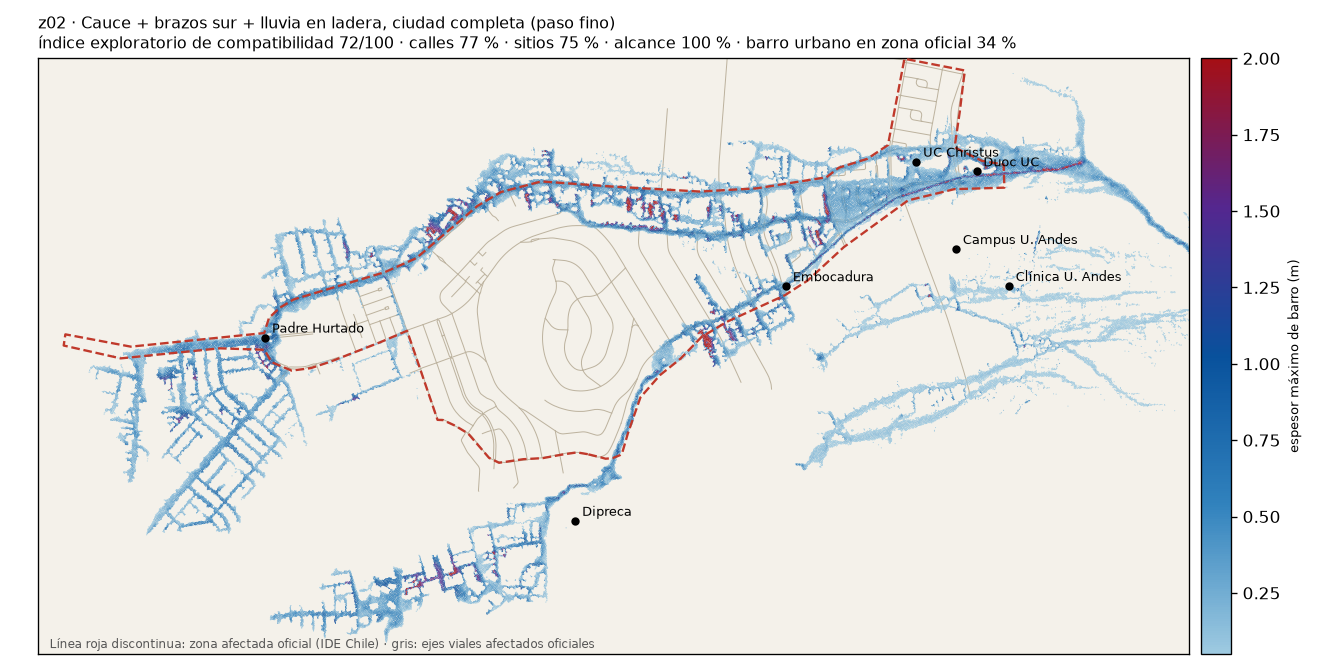
\includegraphics[width=\textwidth]{anexo/z02}\caption{Simulación z02 (cauce principal, brazos sur y lluvia en la ladera, paso de tiempo fino) sobre la zona afectada oficial de IDE Chile (línea roja discontinua) y los ejes viales afectados (gris) \citep{bbnn2026visor}. Colores: espesor máximo simulado.}\label{fig:ide}\end{figure}

\subsection{Ronda del 11 de octubre y prueba con observaciones reservadas}\label{sec:res-ronda}
\paragraph{Ensayos sobre la extensión y el doble conteo.} Cada ensayo cambió un factor de la hipótesis principal:
\begin{itemize}
\item \textbf{Barro algo más concentrado} (v25, $C_v=0{,}43$): no reduce el barro fuera de la zona afectada oficial (fracción dentro de la zona: 0,346, frente a 0,344 en z02).
\item \textbf{Mayor rugosidad fuera de las calles} (v27; $K=800$ y $n=0{,}08$): es el único que la reduce algo (0,388).
\item \textbf{Lluvia aplicada solo fuera de las cuencas aportantes} (v28): elimina el doble conteo sin cambiar los indicadores. La afectación junto a la Clínica Universidad de los Andes se mantiene (\SI{0,15}{m}).
\item \textbf{Reología por zona} (v29; $C_v=0{,}27$ en el faldeo): no cambia los componentes del índice.
\end{itemize}
En los cuatro, el componente «sitios» llega a 1,00 porque el punto de control del campus supera \SI{5}{cm} con el paso de tiempo normal (\SIrange{0,06}{0,15}{m}); en las referencias con paso fino disponibles para esa selección, ese punto queda en \SI{0,01}{m} (v19, z02). La verificación posterior propia de v29 (z29) sí mantiene el punto mojado (sección~\ref{sec:res-posterior}). Según una regla registrada antes de elegir el candidato (protocolo de validación, enmienda~1), ese componente se calcula sin el punto del campus. Así, los índices de 78--79 quedan en 72--73. Todas las configuraciones empatan dentro de tres puntos, y se selecciona z02, verificada con paso fino.

\paragraph{Microsimulaciones del campus.} Se ensayaron desbordes de \SI{20}{m^3/s} y \SI{40}{m^3/s} en la parte alta de Álvaro del Portillo, con barros de $C_v$ 0,25 a 0,40 y triángulos de \SI{8}{m^2} (m20, mk20, ml20, ml40). En todos, el flujo baja por la avenida y sale del dominio sin alcanzar la Biblioteca. El punto de desborde queda fuera de la cuenca local de la Biblioteca, a unos \SI{220}{m} de su límite, de modo que con este relieve ese flujo drena hacia otro lado. Las variantes de escorrentía generada dentro de esa cuenca local y de un camino de entrada que el terreno de \SI{30}{m} no resuelve se ensayaron después: las microsimulaciones y m36 reproducen la entrada por el claro al patio (sección~\ref{sec:res-posterior}). Su validación independiente permanece sin probar (sección~\ref{sec:conclusiones}).

\paragraph{Prueba con observaciones reservadas.} El procedimiento fue:
\begin{itemize}
\item \textbf{Reserva y métrica previas.} Antes de cruzarla con el modelo, se reservaron los 49 equipamientos afectados de la capa oficial que no coinciden con recintos de ajuste. Se fijó la métrica: fracción de puntos con barro simulado de más de \SI{5}{cm} a \SI{15}{m} o menos. El criterio favorable era al menos 0,70 y superar a las referencias v01 (solo cauce principal) y e03 (solo desborde en la embocadura).
\item \textbf{Ejecución única.} La prueba se ejecutó una sola vez sobre el candidato congelado.
\item \textbf{Resultados.} z02 alcanza 19 de 49 puntos (0,39), v01 los mismos 19 y e03 ninguno.
\end{itemize}
\textbf{El resultado es desfavorable.} Se informa sin modificar el modelo. En un diagnóstico posterior, que no cambia el veredicto:
\begin{itemize}
\item la distancia mediana a la celda con barro más cercana es de \SI{32}{m};
\item 16 puntos quedan a más de \SI{100}{m};
\item z02 moja cerca del \SI{20}{\percent} del área de la zona afectada oficial y el \SI{32}{\percent} de sus predios afectados.
\end{itemize}
Es decir, además de extenderse fuera de la zona afectada oficial, la reconstrucción deja sin barro partes importantes de ella. Parte de los puntos no alcanzados corresponden a instalaciones de servicio; su inclusión en la capa oficial no permite inferir el proceso físico de afectación. La prueba es solo parcialmente independiente, porque los puntos están en la zona usada por el índice.

\subsection{Ensayos posteriores a la prueba reservada}\label{sec:res-posterior}
Los ensayos de esta sección terminaron después de congelar el candidato y ejecutar la prueba reservada (sección~\ref{sec:res-ronda}). Sus resultados son de ajuste y no modifican el veredicto de esa prueba. Cualquier nueva selección requerirá observaciones reservadas nuevas.

\paragraph{Casas porosas.} En v26 los edificios de la zona afectada oficial dejan entrar el barro y lo retienen: piso a la cota del terreno más \SI{0,3}{m}, con alta resistencia. Con esta representación:
\begin{itemize}
\item la fracción del barro urbano dentro de la zona afectada oficial sube de 0,34 a 0,54;
\item el modelo moja el \SI{36}{\percent} de la zona afectada oficial (\SI{20}{\percent} en z02) y el \SI{40}{\percent} de sus predios afectados;
\item se cumplen los cuatro criterios originales.
\end{itemize}
La repetición con paso fino (z26) confirma un IEC de 76/100, y con la mitad de la resistencia (v30) el resultado casi no cambia. Como contrapartida, al retener barro en los lotes, el espesor junto a la urgencia de la Clínica UC Christus baja a \SI{0,30}{m}, frente a cerca de \SI{1}{m} informado por Cadena 3.

\paragraph{Faldeo más líquido.} Con la reología por zona ($C_v=0{,}27$ en el faldeo), el punto de control del campus se moja también con paso fino (\SI{0,09}{m} en z29), a diferencia de z02 (\SI{0,01}{m}). El IEC verificado es 78/100.

\paragraph{Cuadratura de la concentración.} Se usaron cinco nodos de Gauss para $C_v=0{,}20+0{,}30X$, $X\sim\mathrm{Beta}(3,2)$, sobre la configuración sin doble conteo. Los valores, condicionados a esa distribución de creencia y sin ser probabilidades de inundación, son:
\begin{itemize}
\item área esperada con más de \SI{5}{cm}: \SI{169}{ha} (\SI{144,5}{ha} mojadas en todos los nodos y \SI{192,3}{ha} en alguno);
\item espesor máximo esperado promediado: \SI{0,38}{m}, con una desviación entre nodos de \SI{0,027}{m};
\item IEC entre 71 y 73 en todo el rango.
\end{itemize}
La concentración mueve sobre todo los bordes de la extensión, no los espesores.

\paragraph{Campus y Av.\ La Plaza Sur.} El autor aportó cinco tipos de información:
\begin{itemize}
\item un video publicado por Meganoticias a las 18:16 del 8 de octubre \citep{meganoticias2026uandes}, con agua turbia que baja del bosque y llena un patio hundido junto a un edificio del campus (espesor estimado visualmente en este estudio: unos \SIrange{15}{35}{cm} según las bancas);
\item la ubicación de ese patio y del claro por donde entra el agua;
\item imágenes de Street View que muestran La Plaza Sur con dos calzadas a distinto nivel (aproximadamente \SI{1,5}{m});
\item 81 puntos con cota de Google Earth (diferencia con el modelo: \SI[uncertainty-mode=separate,retain-explicit-plus=true]{+1,1 +- 1,8}{m});
\item los trazados de un camino de tierra recto que baja del cerro a La Plaza Sur y de una entrada secundaria a un estacionamiento.
\end{itemize}
Con microsimulaciones (triángulos de \SI{8}{m^2}, lluvia de \SI{35}{mm/h} durante una hora y agua turbia, $C_v=0{,}10$) se obtuvo lo siguiente:
\begin{itemize}
\item el desborde simulado de Álvaro del Portillo no llega al patio con ninguno de los fluidos ensayados: el punto de desborde queda fuera de su cuenca local;
\item la lluvia local sobre el terreno sin modificar deja \SI{0,15}{m} en el patio. Un lomo de \SI{0,3}{m} del relieve, menor que su precisión vertical, desvía el agua del claro a otro punto bajo;
\item al tallar el paso del claro al patio, el patio llega a \SIrange{0,17}{0,30}{m}, dentro del rango del video;
\item al tallar la calzada baja de La Plaza Sur, la avenida tiene más de \SI{5}{cm} en el \SIrange{81}{87}{\percent} de sus puntos, frente al \SIrange{12}{20}{\percent} sin tallar. Es compatible con lo que El Dínamo atribuye a Senapred sobre las calles más afectadas;
\item el camino del cerro agrega agua donde llega a la avenida.
\end{itemize}
La configuración resultante supone escorrentía turbia de la ladera y del cerro: caminos de tierra, un \emph{bike park} con pistas desnudas y la superficie clasificada como quemada. En el modelo, la avenida encauza el agua hacia el norte y esta entra a la universidad por el claro. Se representa con propiedades distintas del barro espeso de la rama principal; no se identifica así el proceso ocurrido durante el evento. Los tallados son representaciones gruesas basadas en observaciones aportadas, no mediciones.

\paragraph{Hipótesis integrada.} v32 reúne lo anterior a escala de ciudad:
\begin{itemize}
\item casas porosas;
\item faldeo con $C_v=0{,}10$ y resto con $C_v=0{,}40$;
\item camino, La Plaza Sur y entradas a la universidad tallados;
\item lluvia de \SI{35}{mm/h} sobre todo el faldeo, fuera de las cuencas aportantes.
\end{itemize}
Resultados de v32:
\begin{itemize}
\item IEC bruto de 82/100: calles 0,77; sitios 1,00; alcance 1,00; zona afectada oficial 0,51. Cumple los cuatro criterios originales;
\item el punto del campus llega a \SI{0,61}{m};
\item La Plaza Sur tiene más de \SI{5}{cm} en el \SI{46}{\percent} de sus puntos;
\item el agua llega por el claro al patio (\SI{0,07}{m}) y al estacionamiento (\SI{0,05}{m}). Es menos que en las microsimulaciones; la diferencia de resolución se examinó después con m36.
\end{itemize}
La repetición con paso fino (z32) mantiene el IEC en 82/100 y el campus en \SI{0,61}{m}: el resultado queda verificado. Está condicionado, además, a una lluvia de \SI{35}{mm/h} durante una hora, que supera la intensidad medida (máximo de aproximadamente \SI{22}{mm/h} en \SI{30}{min} en Río Molina).

\paragraph{Sensibilidad a la lluvia.} El CR2 informa registros de Río Molina de unos \SI{32}{mm} entre las 15:00 y las 19:00, con un máximo de \SI{10,9}{mm} en \SI{30}{min}. Con la lluvia medida (v33: \SI{8}{mm/h} durante \SI{4}{h}):
\begin{itemize}
\item el IEC de la hipótesis integrada baja a 79/100 y la fracción dentro de la zona afectada oficial a 0,41: la lluvia larga moja más superficie fina fuera de ella;
\item el campus sigue mojado (\SI{0,48}{m});
\item en La Plaza Sur y el patio la señal se debilita, aunque la malla de ciudad la subestima.
\end{itemize}
A escala de detalle, con \SIlist{15;25;35}{mm/h}, el mecanismo La Plaza Sur $\rightarrow$ claro $\rightarrow$ patio aparece en los tres casos: el patio queda en \SIrange{0,12}{0,17}{m} y La Plaza Sur se moja en el \SIrange{41}{87}{\percent}. No depende de excluir las cuencas aportantes ni del aporte de las quebradas cortas del sur. Por eso los resultados de ajuste se informan como rango según la lluvia: IEC de 79 a 82.

Un primer intento (v31), que inyectaba el cauce principal aguas arriba de una franja densa de árboles señalada por el autor, se descartó: el punto de inyección no estaba en el fondo de la quebrada y el flujo se escapó hacia el norte.

\paragraph{Lluvia con su distribución temporal registrada.} Con la lluvia de Río Molina cada \SI{30}{min} (\SI{31,8}{mm} entre las 15:00 y las 19:00, digitalizada de la figura del CR2 y consistente con sus totales), con el pico del hidrograma al final del tramo más intenso (p34b, corregida):
\begin{itemize}
\item la hipótesis integrada obtiene un IEC de 81 (calles 0,77; zona afectada oficial 0,48);
\item el campus llega a \SI{0,49}{m} y La Plaza Sur tiene barro en el \SI{33}{\percent} de sus puntos;
\item la superficie con más de \SI{5}{cm} es de \SI{222}{ha}.
\end{itemize}
El pulso concentra el agua y moja menos superficie fuera de la zona afectada oficial que la misma lluvia repartida en \SI{4}{h} (79).

Con triángulos de \SI{8}{m^2} en el campus y La Plaza Sur (m36), la simulación de ciudad reproduce el mecanismo de las microsimulaciones:
\begin{itemize}
\item el patio llega a \SI{0,17}{m}, dentro del rango del video, y el claro a \SI{0,19}{m};
\item La Plaza Sur tiene barro en el \SI{58}{\percent} de sus puntos;
\item el resto de la ciudad casi no cambia (IEC 82; \SI{220}{ha} mojadas).
\end{itemize}
La diferencia entre escalas se debía a la resolución de la malla, no al proceso. m36 se lanzó antes de la corrección del paso de tiempo y tiene un residuo de \SI[retain-explicit-plus=true]{+0,6}{\percent}.

\paragraph{Artefacto numérico detectado y corregido.} En las corridas de este grupo (p34, d39, f35, f38, arc y art), los hidrogramas comienzan a las \SI{2,8}{h} para coincidir con el pulso de lluvia. Mientras tanto, el dominio está casi seco y el modelo toma pasos de tiempo muy grandes sobre la película de lluvia. Entre los minutos 1 y 2, la corrección de profundidades negativas creó unos \SI{7500}{m^3} en el faldeo: un residuo de balance de \SI[retain-explicit-plus=true]{+2,1}{\percent} (\SI[retain-explicit-plus=true]{+3,1}{\percent} en las corridas sin incendio). Las seis corridas comparten el artefacto, de modo que las comparaciones entre ellas siguen siendo válidas. Con un paso de tiempo máximo de \SI{0,5}{s}, el residuo vuelve a cero. Las repeticiones corregidas (p34b, f35b y f38b) tienen un residuo de \SI{0,00}{\percent} y confirman las conclusiones: los valores cambian en pocas hectáreas y centésimas de metro. Se informan los valores corregidos.

\paragraph{Obstáculo hipotético de árboles.} El autor marcó una línea de árboles que baja por la quebrada principal (\SI{1046}{m} a \SI{994}{m} de cota en unos \SI{720}{m}) y una acumulación al final, poco antes de la salida al abanico. Se talló un cauce por esa línea, con el hidrograma del cauce principal inyectado aguas arriba (arc), y se agregó la acumulación como un obstáculo de altura supuesta de \SI{3}{m} (art). Resultados del modelo:
\begin{itemize}
\item el obstáculo supuesto no desvía el flujo simulado hacia el sur: Álvaro del Portillo y el campus tienen la misma superficie mojada en ambos casos (\SI{20,2}{ha});
\item retiene y reparte barro junto al abanico (unas \SI{59}{ha} más mojadas) y el barro llega menos lejos hacia el poniente (unas \SI{70}{ha} más secas);
\item el IEC casi no cambia (78 frente a 79).
\end{itemize}

\paragraph{\emph{Bike park}.} Con el dominio ampliado al este y al sur, con lluvia de \SI{25}{mm/h} y agua turbia, se comparó el terreno con y sin la pista principal del \emph{bike park} tallada hasta el inicio del camino del cerro (mrbt y mrbc). Los resultados son idénticos:
\begin{itemize}
\item La Plaza Sur con barro en el \SI{78}{\percent} de sus puntos;
\item \SI{0,26}{m} al final del camino, \SI{0,14}{m} en el claro y \SI{0,11}{m} en el patio.
\end{itemize}
En el modelo, con este relieve, el agua de la superficie del \emph{bike park} escurre hacia el camino, con o sin la pista tallada. Incluir toda la ladera alta en la lluvia sí agrega agua: frente a mrd25, La Plaza Sur pasa del \SI{69}{\percent} al \SI{78}{\percent}. El aporte de sedimento de las pistas no puede evaluarse, porque el modelo no simula erosión.

\paragraph{Porosidad por tamaño.} Si solo las casas de \SI{250}{m^2} o menos dejan entrar el barro (d39), el espesor junto a la Clínica UC Christus sigue en \SI{0,31}{m}. El menor espesor calculado allí se debe al almacenamiento representado en las casas de aguas arriba, no al tamaño de los edificios.

\subsection{Campus de la Universidad de los Andes}\label{sec:res-campus}
El vicerrector de la universidad ubicó el desborde en la quebrada del costado norte del campus, que colinda con General Blanche, por donde bajó la masa de barro \citep{cooperativa2026}, y Carabineros ubicó la zona cero en Álvaro del Portillo con Av.\ La Plaza \citep{latercera2026zonacero}; un video difundido en redes muestra barro en el Aula Magna \citep{quintaconectado2026}. En el modelo con el brazo sur por el cauce oficial (v19), el barro llega a la parte alta de Álvaro del Portillo (\SI{0,49}{m} donde termina el cauce y \SI{0,13}{m} en la avenida) y baja por ella hacia La Plaza y General Blanche, en concordancia con ambos relatos. No cruza, en cambio, el bosque que separa la avenida de la biblioteca, aunque el terreno desciende de \SI{936,5}{m} a \SI{927,4}{m} hacia una depresión junto al edificio. Se ensayaron inicialmente tres mecanismos: (i) \emph{aporte de quebradas secundarias}: la delimitación sobre el terreno asigna a la biblioteca una cuenca local de \SI{11,3}{ha}, ajena a las cuencas aportantes, de la que solo el \SI{57}{\percent} recibe lluvia en las simulaciones principales; (ii) \emph{escorrentía más líquida en el faldeo}: en las imágenes del campus citadas no se distinguen piedras ni escombros urbanos; se ensayó por ello un flujo más diluido que en la rama principal; y (iii) \emph{redistribución local} por taludes, senderos y accesos. Para ello se usaron microsimulaciones locales de unos \SI{800}{m} $\times$ \SI{720}{m} con triángulos de \SI{8}{m^2}, con desbordes de \SI{10}{m^3/s} a \SI{40}{m^3/s} en la parte alta de Álvaro del Portillo, barros de $C_v$ 0,25, 0,30 y 0,40, y lluvia sobre toda la cuenca local. También se usó una simulación de la ciudad completa (v29) con reología por zona: $C_v=0{,}27$ en el faldeo y $C_v=0{,}43$ en el resto, más la lluvia aplicada solo fuera de las cuencas aportantes. La reología por zona es una representación intermedia: asigna un barro distinto según la ubicación, pero no representa la evolución de la concentración durante el recorrido. Los ensayos posteriores reprodujeron la entrada por el claro al patio; m36 calcula \SI{0,17}{m} en el patio y moja el \SI{58}{\percent} de La Plaza Sur (sección~\ref{sec:res-posterior}).

\subsection{Terreno anterior}\label{sec:res-terreno}
El dominio cubre \SI{5,9}{km} por \SI{3,4}{km} con una retícula de \SI{4}{m}. Contiene 1.103 edificios representados como bloques, con altura media de \SI{6,2}{m} y máxima de \SI{39}{m}: 82 alturas obtenidas de la diferencia entre superficie y terreno, 26 de los pisos registrados y 995 supuestas en \SI{6}{m}. Se excluyeron cuatro polígonos que corresponden a recintos (complejos deportivos y un centro comercial) y no a volúmenes construidos. En el terreno base, el cauce abierto del parque lineal entre el abanico y Francisco Bulnes Correa queda prácticamente plano (relieve transversal de $\pm\SI{0,5}{m}$). En el terreno fotogramétrico del año 2014 \citep{hussain2021}, con resolución efectiva de \SI{8}{m} a \SI{10}{m}, el cauce aparece como una depresión de \SI{1}{m} a \SI{4,5}{m} respecto de sus márgenes. Ese terreno presenta un desfase vertical de \SI{26,7}{m} (diferencia entre referencias elipsoidal y geoidal) y depresiones espurias, que se corrigieron antes de usarlo.

\subsection{Verificación numérica}\label{sec:res-verif}
\paragraph{Equilibrio del depósito.} Al detenerse sobre un plano de pendiente 0,05, el depósito satisface el criterio de fluencia: el residuo local $r=\rho_m g h|\nabla(z+h)|/\tau_y$ tiene mediana y percentil 95 iguales a 1,00, sin celdas con $r>1{,}05$. El espesor teórico de reposo es $h_c=\SI{0,1200}{m}$ con $g=\SI{9,8}{m.s^{-2}}$.
\paragraph{Reinicio.} Al agregar mezcla aguas arriba, el frente avanza \SI{26}{m} más que en el control sin aporte. El control, sin embargo, también avanza \SI{19}{m} en \SI{900}{s}, y la deriva del frente detenido es de \SI{6,7}{m} en los últimos \SI{300}{s}. Ese deslizamiento residual proviene del paso fraccionado y disminuye al reducir el paso de tiempo.
\paragraph{Convergencia.} Con CFL~0,25, el alcance converge al refinar la malla: \SIlist{354;345,7;341,2}{m} para celdas de \SIlist{4;2;1}{m}, con un valor extrapolado de unos \SI{337}{m}. Con celdas de \SI{2}{m}, el alcance disminuye al reducir el número de Courant: \SIlist{431;374;346;328}{m} para CFL 1; 0,5; 0,25 y 0,1. Es una convergencia de primer orden, con un sesgo de \SI[retain-explicit-plus=true]{+30}{\percent} para CFL~1.
\paragraph{Convergencia en el dominio urbano.} En el terreno con las 42.018 huellas de edificios, la simulación de \SI{300000}{m^3} por el cauce principal se repitió con CFL~0,25. Respecto de CFL~1, la diferencia de espesor máximo tiene mediana de \SI{2}{mm} y percentil 95 de \SI{9}{mm}; el \SI{99}{\percent} de las celdas coincide en mojado o seco; la llegada del frente difiere en menos de \SI{20}{s}, y la distancia mínima a Padre Hurtado es la misma (\SI{96}{m}). En la simulación de ciudad, el frente se detiene por la geometría representada de calles y edificios y no por el deslizamiento residual del ensayo en plano. La comparación temporal urbana realizada no muestra un sesgo de esa magnitud en los indicadores examinados.
\paragraph{Doble conteo de la lluvia en la ladera.} La lluvia sobre la ladera se aplica en un polígono de \SI{1,048}{km^2} y aporta \SI{36680}{m^3} además de los hidrogramas. El \SI{74}{\percent} de ese polígono está fuera de las cuencas aportantes, cuya escorrentía ya entra por los hidrogramas; el \SI{26}{\percent} restante se superpone con parte de S1 (\SI{0,096}{km^2}) y con toda S2 (\SI{0,172}{km^2}), lo que cuenta dos veces unos \SI{9400}{m^3}, el \SI{2,8}{\percent} del volumen total, concentrados en el entorno de la Clínica Universidad de los Andes. La simulación v28 repite la hipótesis principal aplicando la lluvia solo fuera de las cuencas (\SI{27290}{m^3}) para cuantificar su efecto.
\paragraph{Balance de volumen.} En todas las simulaciones del dominio urbano, el volumen en la malla coincide con el aportado, menos el retirado por el colector y el que sale por los bordes, con un residuo menor a \SI{0,01}{\percent}. Hay excepciones documentadas. En las seis corridas con los hidrogramas desplazados (p34, d39, f35, f38, arc y art), la corrección de profundidades negativas creó entre un \SI{2,1}{\percent} y un \SI{3,1}{\percent} de masa (sección~\ref{sec:res-posterior}); se corrigió, y las repeticiones p34b, f35b y f38b dan \SI{0,00}{\percent}. En m36, con malla fina en el campus y lanzada antes de la corrección, el residuo es de \SI[retain-explicit-plus=true]{+0,6}{\percent}. En algunas microsimulaciones del campus con lluvia, el residuo llega hasta un \SI{3,2}{\percent}, y se informa en cada caso. Una versión anterior del borde de salida generaba masa espuria al llegar el frente al límite sur, con un aumento de hasta un \SI{20}{\percent}; esas simulaciones se descartaron y se repitieron con un borde de solo salida.

\subsection{Estimación independiente del volumen}\label{sec:res-volumen}
La delimitación sobre el modelo de elevación calcula una cuenca aportante de \SI{10,1}{km^2}: el cauce principal (\SI{8,04}{km^2}, relieve de \SI{1376}{m}), el cauce sur (\SI{1,90}{km^2}) y las quebradas menores (\SI{0,17}{km^2}). Con el balance lluvia--escorrentía, la mediana del volumen de mezcla es de \SI{151000}{m^3}, con percentiles 5 y 95 de \SI{67000}{m^3} y \SI{310000}{m^3}. En el cálculo inicial del modelo para cuencas quemadas \citep{gartner2014}, con severidad supuesta, la mediana fue de \SI{374000}{m^3}, con percentiles de \SI{61000}{m^3} y \SI{2,3e6}{m^3}; al usar la severidad estimada con dNBR se obtuvo \SI{148000}{m^3} (sección~\ref{sec:res-incendio}). Con \SI{151000}{m^3}, la relación de \citet{mizuyama1992} da $Q_p\approx\SI{230}{m^3/s}$.

Con el escenario de suelo saturado, la mediana sube a \SI{295000}{m^3}, con percentiles 5 y 95 de \SI{181000}{m^3} y \SI{468000}{m^3}. El límite superior calculado para la fusión de nieve es de unos \SI{15000}{m^3}, menos del \SI{5}{\percent}: el análisis satelital descrito no detectó manto previo en la parte despejada de la cuenca y la hipsometría calcula el \SI{90}{\percent} de su superficie bajo \SI{1800}{m}. En los escenarios de isoterma, cambia el área supuesta que recibe lluvia: si la cota de nieve se toma unos \SI{300}{m} bajo la isoterma, en el cálculo, una isoterma supuesta de \SI{2000}{m} deja \SI{8,2}{km^2} bajo lluvia (\SI{81}{\percent}), una de \SI{1800}{m}, \SI{6,0}{km^2} (\SI{59}{\percent}), y una de \SI{1500}{m}, \SI{1,7}{km^2} (\SI{16}{\percent}); con la isoterma informada para el 8 de octubre se supone lluvia sobre los \SI{10,1}{km^2}. Con la misma lluvia supuesta, los escenarios de isoterma típica calculan entre un \SI{20}{\percent} y un \SI{40}{\percent} menos de agua en el pulso.

\subsection{Severidad estimada del incendio y escenarios de volumen}\label{sec:res-incendio}
La severidad se calculó con el índice dNBR de Sentinel-2 \citep{keybenson2006}, comparando una escena sin nubes del 23 de diciembre de 2025, seis días antes del inicio del incendio, con otra del 6 de febrero de 2026 (figura~\ref{fig:dnbr}). La distribución espacial coincide con la que publicó el CR2 \citep{cr2_2026}. De los \SI{10,1}{km^2} de las cuencas aportantes:
\begin{itemize}
\item \SI{8,2}{km^2} (\SI{82}{\percent}) muestran señal de quema (dNBR de 0,10 o más);
\item la severidad es mayoritariamente baja (\SI{2,8}{km^2}) o moderada-baja (\SI{4,5}{km^2});
\item solo \SI{1,0}{km^2} (\SI{10}{\percent}) es de severidad moderada-alta o alta, casi todo en el cauce principal.
\end{itemize}
Los umbrales de clase se calibraron en bosques de Norteamérica y la imagen posterior tiene cinco semanas de rebrote, por lo que la severidad puede estar subestimada en el matorral esclerófilo.

\emph{Corrección del volumen empírico.} El modelo de \citet{gartner2014} se había aplicado con una fracción de severidad moderada-alta supuesta entre \SI{30}{\percent} y \SI{90}{\percent} (sección~\ref{sec:res-volumen}). Con la severidad estimada por satélite para la entrada $B_{mh}$, su mediana de volumen de mezcla baja de \SI{374000}{m^3} a \SI{148000}{m^3}, con percentiles 5 y 95 de \SI{25000}{m^3} y \SI{858000}{m^3}. El balance lluvia--escorrentía no depende de ese supuesto.

\emph{Comparación de escenarios con y sin incendio.} En el balance de suelo saturado, el coeficiente de escorrentía se asignó por clase de severidad:
\begin{itemize}
\item $C_u$ entre 0,40 y 0,60 en lo no quemado;
\item $C_u$ más 0,05--0,15 en severidad baja, 0,15--0,30 en moderada-baja y 0,25--0,45 en moderada-alta o alta, por la hidrofobicidad y la pérdida de cobertura \citep{moody2013};
\item $C_v$ entre 0,30 y 0,50 con incendio y entre 0,20 y 0,35 sin incendio.
\end{itemize}
En el escenario sin incendio se asigna $C_u$ a toda la superficie de la cuenca. Estos incrementos son supuestos, no mediciones. Con ellos, el coeficiente efectivo pasa de 0,50 sin incendio a 0,66 con incendio, y el escenario sin incendio calcula para el pulso:
\begin{itemize}
\item el \SI{76}{\percent} del agua (\SIrange{70}{81}{\percent});
\item el \SI{62}{\percent} del volumen de barro (\SIrange{51}{76}{\percent}), es decir, una mediana de \SI{163000}{m^3} en vez de \SI{262000}{m^3};
\item el \SI{43}{\percent} de los sólidos (\SIrange{25}{74}{\percent}).
\end{itemize}
Con el modelo M1 de \citet{staley2017}, que estima la probabilidad de que una tormenta genere un flujo de detritos en una cuenca quemada, la lluvia de \SI{15}{min} inferida de Río Molina da una probabilidad mediana de 0,28 con incendio y de 0,07 sin él. Ese modelo fue calibrado en el oeste de Estados Unidos y su uso aquí es ilustrativo.

\emph{Respuesta del modelo de ciudad.} Se repitió la hipótesis integrada con la lluvia medida y el volumen sin incendio, es decir, los \SI{300000}{m^3} del modelo multiplicados por la razón mediana del balance sin y con incendio (0,62): \SI{187000}{m^3}, con $Q_p=\SI{172}{m^3/s}$ según la relación de \citet{mizuyama1992} (f35b, repetición corregida de f35), y además con un barro más fluido, $C_v=0{,}25$ (f38b, repetición corregida de f38). Frente a la misma configuración con incendio (p34b, corregida):
\begin{itemize}
\item la superficie con más de \SI{5}{cm} baja de \SI{222}{ha} a \SIrange{179}{193}{ha} (\SIrange{13}{19}{\percent} menos);
\item la fracción de calles con barro baja de 0,77 a 0,70--0,73;
\item el espesor junto a la Clínica UC Christus baja de \SI{0,30}{m} a \SIrange{0,19}{0,23}{m}.
\end{itemize}
El IEC queda en 80--82, frente a 81 con incendio. La métrica de la zona afectada oficial mejora cuando hay menos barro y compensa la pérdida de calles. Estos valores corresponden a las repeticiones corregidas (p34b, f35b y f38b).

\begin{figure}[htbp]\centering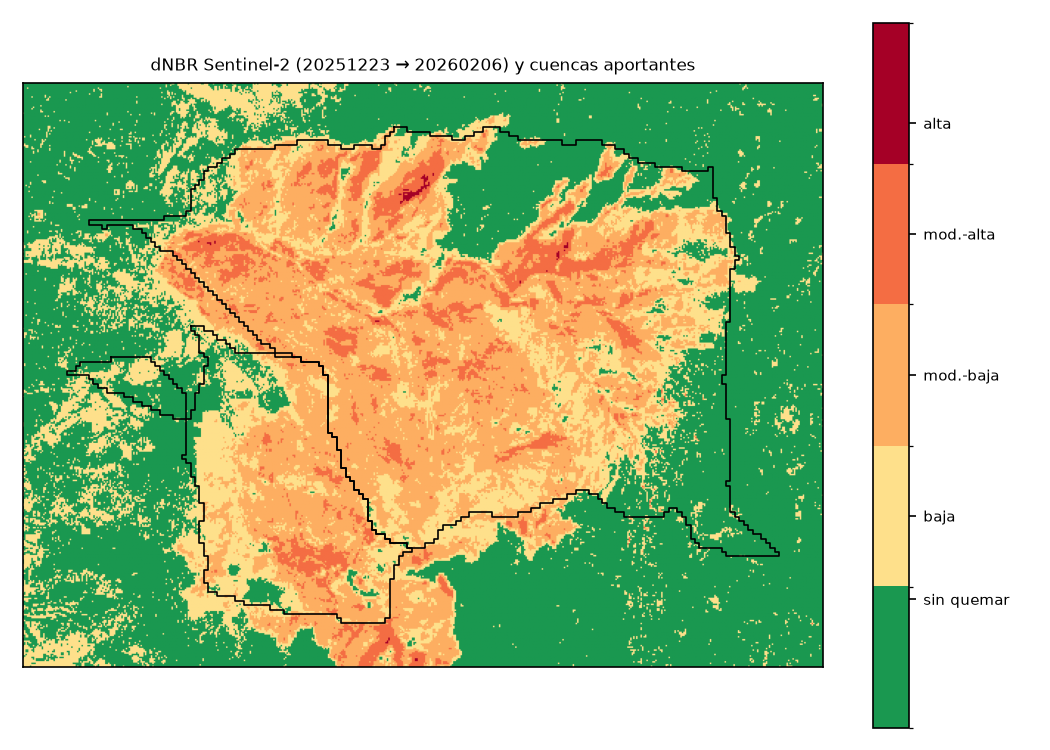
\includegraphics[width=.85\textwidth]{dnbr}\caption{Severidad estimada del incendio de diciembre de 2025 según el índice normalizado de área quemada diferencial (dNBR) de Sentinel-2 (23 de diciembre de 2025 y 6 de febrero de 2026) y límites de las cuencas aportantes (cauce principal al norte, brazo sur y quebradas menores).}\label{fig:dnbr}\end{figure}

\subsection{Cribado inicial con el terreno anterior}\label{sec:res-calib}
\begin{table}[htbp]\centering\small
\caption{Primera generación (9 de octubre de 2026), con el terreno anterior de 1.103 edificios: fracción de puntos de control con espesor máximo simulado mayor a \SI{5}{cm}, por calle, y espesor máximo en un radio de \SI{40}{m} de cada sitio. Las capacidades del colector son supuestas; no describen la obra real. Todas las simulaciones usan Glenwood~2b, $C_v=0{,}40$ y $Q_p=\SI{250}{m^3/s}$, salvo d03 ($Q_p=\SI{100}{m^3/s}$). LP: La Plaza (Álvaro del Portillo--Camino El Alba); GB: General Blanche (San Carlos de Apoquindo--Las Condesas); CEA: Camino El Alba; QH: Quebrada Honda; LPS: La Plaza Sur; UCC: Clínica UC Christus; CUA: Clínica Universidad de los Andes; Duoc: sede Duoc UC; dPH: distancia mínima del barro al cruce de General Blanche con Padre Hurtado.}\label{tab:hipotesis}
{\setlength{\tabcolsep}{4pt}\begin{adjustbox}{max width=\textwidth}\begin{tabular}{llrrrrrrrrr}\toprule
Hipótesis & $V$ (mil \si{m^3}) & LP & GB & CEA & QH & LPS & UCC (\si{m}) & CUA (\si{m}) & Duoc (\si{m}) & dPH (\si{m})\\\midrule
H3 & 80 & 0,87 & 0,86 & 0,61 & 0,00 & 0,00 & 0,22 & 0,00 & 0,42 & 1160\\
H1 & 150 & 0,91 & 0,92 & 0,85 & 0,00 & 0,00 & 0,42 & 0,00 & 0,55 & 366\\
H3 & 150 & 0,88 & 0,92 & 0,78 & 0,00 & 0,00 & 0,39 & 0,00 & 0,53 & 516\\
H3 & 300 & 0,91 & 0,93 & 0,96 & 0,00 & 0,00 & 0,42 & 0,00 & 0,54 & 4\\
H2 & 150 & 0,00 & 0,00 & 0,00 & 0,69 & 0,00 & 0,00 & 0,00 & 0,00 & 856\\
H4, $f_\mathrm{sup}=0{,}5$ & 150 & 0,88 & 0,88 & 0,57 & 0,66 & 0,00 & 0,26 & 0,00 & 0,46 & 1007\\
H4, $f_\mathrm{sup}=0{,}9$ & 150 & 0,88 & 0,91 & 0,68 & 0,54 & 0,00 & 0,35 & 0,00 & 0,52 & 816\\
H5 (H4 + lluvia de \SI{20}{mm/h}) & 150 & 0,88 & 0,88 & 0,57 & 0,66 & 0,00 & 0,26 & 0,06 & 0,46 & 1005\\
H1, cauce tallado, sin colector & 150 & 0,89 & 0,94 & 0,87 & 0,55 & 0,00 & 0,31 & 0,00 & 1,63 & 338\\
\quad ídem, colector \SI{10}{m^3/s} & 150 & 0,89 & 0,94 & 0,87 & 0,43 & 0,00 & 0,31 & 0,00 & 1,63 & 338\\
\quad ídem, colector \SI{30}{m^3/s} & 150 & 0,89 & 0,94 & 0,87 & 0,01 & 0,00 & 0,31 & 0,00 & 1,63 & 338\\
\bottomrule\end{tabular}\end{adjustbox}}
\end{table}

La tabla~\ref{tab:hipotesis} resume las simulaciones de cribado. Se observan cuatro regularidades:
\begin{enumerate}
\item \textbf{Corredores del abanico.} La Plaza, Mons.\ Álvaro del Portillo, Av.\ San Carlos de Apoquindo, el tramo alto de General Blanche y Camino El Alba superan el umbral en el \SIrange{85}{100}{\percent} de sus puntos en todas las hipótesis con salida en el abanico, para volúmenes entre \SI{80000}{m^3} y \SI{300000}{m^3}. Duoc UC y la Clínica UC Christus quedan alcanzados en todas ellas, con espesores de \SI{0,4}{m} a \SI{1,6}{m} y de \SI{0,2}{m} a \SI{0,4}{m}, respectivamente.
\item \textbf{Quebrada Honda.} En el cribado, esta calle solo supera el umbral cuando el flujo simulado sale a la superficie en la embocadura del colector de Francisco Bulnes Correa. Eso ocurre si se impone una fuente allí (H2, H4) o si el terreno representa el cauce abierto que conduce el flujo hasta la embocadura y el sumidero del modelo no lo retira. En esos ensayos basta con que salga allí el \SI{8}{\percent} del volumen.
\item \textbf{Capacidad del colector (terreno anterior; superado).} Con el cauce representado y solo 1.103 edificios, a la embocadura llegan \SI{12800}{m^3}, con un caudal máximo de \SI{16,5}{m^3/s}; en ese escenario, el sumidero del modelo con capacidad supuesta de \SI{30}{m^3/s} o \SI{100}{m^3/s} los retira y Quebrada Honda queda seca (\SI{1}{\percent}). Con la ciudad completa esta conclusión cambia: el caudal calculado sube a unos \SI{65}{m^3/s} y una capacidad supuesta de \SI{30}{m^3/s} deja flujo superficial (sección~\ref{sec:res-colector}). Con capacidad supuesta de \SI{10}{m^3/s}, el modelo calcula un desborde de unos \SI{2600}{m^3} y Quebrada Honda se moja en el \SI{43}{\percent} de sus puntos (figura~\ref{fig:colector}).
\item \textbf{Sector sur.} Ninguna de las simulaciones de la tabla~\ref{tab:hipotesis} moja la Av.\ La Plaza Sur ni el campus de la Universidad de los Andes. Solo la lluvia sobre la ladera oriente (H5) alcanza la Clínica Universidad de los Andes, con \SI{6}{cm} en su entorno, lo que coincide con la declaración de la clínica recogida por Radio La Señal de que la afectación fue exterior.
\end{enumerate}
Con el terreno anterior, ninguna simulación cumple los cuatro criterios de aceptación fijados de antemano (sección~\ref{sec:calib}). El criterio de sitios no se cumple en ninguna, porque no se alcanza el campus, y el de alcance no se cumple en las de \SI{150000}{m^3}.

\begin{figure}[htbp]\centering
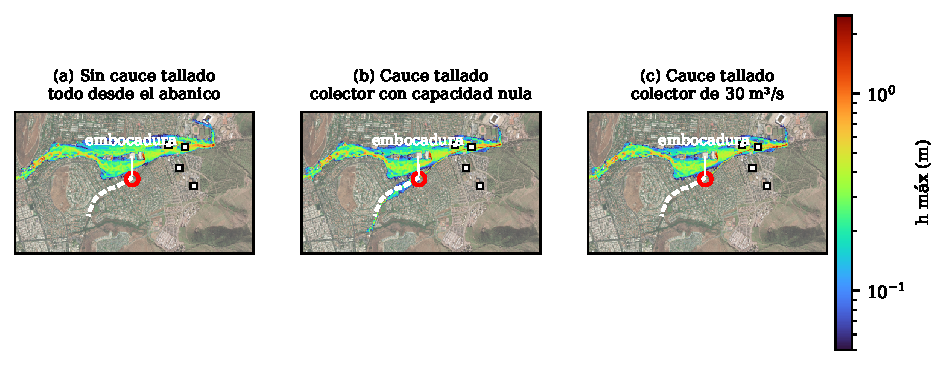
\includegraphics[width=\textwidth]{colector}
\caption{Primera generación (terreno anterior, 1.103 edificios; superada por la sección~\ref{sec:res-colector}). Espesor máximo simulado con \SI{150000}{m^3} saliendo en el abanico. (a) Terreno base: el flujo no alcanza Quebrada Honda (línea blanca discontinua). (b) Cauce del parque lineal tallado y sumidero del modelo con capacidad nula supuesta: el flujo que llega por el cauce a la embocadura (círculo rojo) desborda hacia Quebrada Honda. (c) Mismo terreno con capacidad supuesta del sumidero de \SI{30}{m^3/s}: el modelo retira el flujo que llega y Quebrada Honda queda seca. Los cuadrados indican los sitios con afectación informada por las fuentes de la sección~\ref{sec:evidencia}.}\label{fig:colector}
\end{figure}

\subsection{Contraste con información posterior a las hipótesis}\label{sec:res-contraste}
Después de formular las hipótesis se conocieron tres fuentes que permiten un contraste parcial, aunque no independiente de la prensa:
\begin{itemize}
\item \textbf{Versión preliminar recogida por El Desconcierto} \citep{eldesconcierto2026}: el medio recoge una versión del delegado presidencial sobre la obstrucción del ingreso a dos ductos paralelos en General Blanche y describe una interrupción del funcionamiento de la cámara de decantación de Francisco Bulnes Correa; también recoge un desborde del canal en esa calle informado por Carabineros. Son versiones de la fuente. En los escenarios ensayados, representar aportes superficiales en ambos sectores permite reproducir flujo en el abanico y Quebrada Honda, sin confirmar esas versiones ni el estado de las obras.
\item \textbf{Reporte técnico de Sernageomin sobre el aluvión del 31 de enero de 2026} \citep{sernageomin2026reterm}: describe un corredor único desde el Parque San Carlos de Apoquindo, por el sector de la Universidad de los Andes, hasta Quebrada Honda con Francisco Bulnes Correa, con continuación hacia la quebrada Apoquindo, el Hospital Dipreca y Paul Harris. El reporte describe el canal paralelo a Quebrada Honda colmatado de barro tras ese evento. Coincide con el recorrido del cauce que el modelo necesita representar. El dominio ampliado de la versión vigente ya incluye la continuación hacia Dipreca y Paul Harris.
\item \textbf{Mapa de prensa} \citep{chilevision2026mapa}: traza como vías del aluvión los ejes de Camino El Alba, General Blanche y Quebrada Honda hasta Padre Hurtado. Sobre esas líneas completas, la simulación considerada en ese contraste moja el \SI{92}{\percent} de Camino El Alba, el \SI{40}{\percent} de General Blanche y el \SI{27}{\percent} de Quebrada Honda. El tramo bajo de General Blanche, entre Las Condesas y Padre Hurtado, no se reproduce: el flujo simulado prefiere Camino El Alba en ese tramo.
\end{itemize}

Entre el 9 y el 10 de octubre se conocieron más datos, que se contrastaron sin modificar las simulaciones:
\begin{itemize}
\item \textbf{Lugares con ingreso de barro o agua.} Según las fuentes citadas, Senapred incluye la Av.\ La Plaza Sur entre las tres calles más afectadas; el campus de la Universidad de los Andes tuvo barro y personas retenidas, y la Clínica Universidad de los Andes, un ingreso menor de agua \citep{interferencia2026,cooperativa2026}. En el terreno con edificios, la simulación por el cauce principal no moja ninguno de esos tres puntos. La que agrega los brazos sur y lluvia sobre la ladera da \SI{0,14}{m} junto a la Clínica Universidad de los Andes y moja parte de La Plaza Sur, pero deja el campus con \SI{1}{cm}. Ambas reproducen la Clínica UC Christus (\SI{1,13}{m} a \SI{1,16}{m}, frente a cerca de \SI{1}{m} informado) y la sede Duoc UC (\SI{1,9}{m}).
\item \textbf{Evento del 31 de enero.} Según T13, con \SI{75}{mm} en \SI{1}{h} \SI{20}{min}, una intensidad mucho mayor que la del 8 de octubre, afectó \SI{8}{ha}, cerca de \SI{4}{km} de calles y 11 viviendas \citep{t13_2026mallas}, y el colector de Francisco Bulnes Correa «funcionó muy bien» según la alcaldesa \citep{latercera2026enero}. La diferencia entre los balances informados motiva los escenarios de saturación antecedente y material disponible; no permite establecer su contribución al evento ni compararla causalmente con la intensidad pico.
\item \textbf{Superficie afectada.} Las \SI{253}{ha} informadas por Chicureo Hoy \citep{chicureohoy2026} coinciden con el área del perímetro municipal publicado por la prensa (área calculada: \SI{253,0}{ha}). Es un perímetro de seguridad y no un mapa del barro: dentro de él el barro simulado ocupa cerca de \SI{40}{ha}, porque se concentra en las calles. No se usa para discriminar hipótesis.
\item \textbf{Hospital de la FACh.} Según Interferencia, se informó agua en su servicio de urgencias. Ninguna simulación llega a ese punto, unos \SI{1,3}{km} al norte del recorrido; no se usa como criterio de ajuste. El drenaje urbano por lluvia queda fuera del modelo y no se infiere aquí el origen de esa afectación.
\end{itemize}

\subsection{Indicadores en sitios críticos}\label{sec:res-indicadores}
Primera generación (terreno anterior, simulación e04; no comparable directamente con las simulaciones con la ciudad completa). En la simulación con el cauce tallado y el colector con capacidad nula supuesta, los máximos en un radio de \SI{40}{m} son los siguientes:
\begin{itemize}
\item Duoc UC: \SI{1,6}{m} de espesor, \SI{6,3}{m/s} y \SI{33}{kPa} de presión dinámica; el frente llega al minuto~4.
\item Cruce de General Blanche con San Carlos de Apoquindo: \SI{1,4}{m}, \SI{6,7}{m/s} y \SI{37}{kPa}, al minuto~7.
\item Clínica UC Christus: \SI{0,3}{m} y \SI{1,6}{m/s}, al minuto~9.
\item Embocadura de Francisco Bulnes Correa: \SI{1,6}{m} y \SI{3,9}{m/s}, al minuto~13.
\end{itemize}
Los minutos se cuentan desde el inicio del pulso. Con ese escenario, 170 edificios quedan con barro sobre \SI{5}{cm} junto a su fachada, 46 sobre \SI{0,5}{m} y 11 sobre \SI{1}{m}; 8 reciben una presión dinámica mayor a \SI{10}{kPa}. Estos valores tienen el sesgo de cribado ya señalado y no se han contrastado con mediciones.


\section{Las hipótesis, una por una}\label{sec:recorrido}
Esta sección reúne en un solo hilo lo que las secciones anteriores presentan por separado. Para cada hipótesis indica qué hecho la motivó, cómo se representó en el modelo, qué resultó y en qué estado queda. La tabla~\ref{tab:recorrido} la resume. Un resultado «compatible» significa que el modelo reproduce lo observado con supuestos razonables; no prueba que el evento haya ocurrido así. El índice exploratorio de compatibilidad (IEC) compara hipótesis entre sí con los mismos criterios; no es una validación.

\subsection{Puntos de entrada del flujo ensayados en el modelo}
\paragraph{H1: el cauce principal sale en el abanico.} \emph{Por qué se planteó.} Las primeras informaciones recogidas por Chilevisión e Interferencia situaron el origen en la quebrada que baja al abanico de Álvaro del Portillo, La Plaza y General Blanche, donde la quebrada entra a un ducto bajo la urbanización. El escenario supone que el ducto no recibe flujo y asigna todo el aporte a la superficie desde ese punto. \emph{Cómo se representó.} Un hidrograma triangular de mezcla inyectado en la salida del cauce al abanico. \emph{Qué resultó.} En el modelo con solo el cauce principal (v01), el barro recorre General Blanche y Camino El Alba y llega cerca de Padre Hurtado, pero no reproduce la afectación informada en el sector sur: la Av.\ La Plaza Sur, la Clínica Universidad de los Andes y el campus quedan secos. En la prueba con observaciones reservadas alcanza los mismos 19 de 49 puntos que la hipótesis seleccionada. \emph{Estado.} La entrada por el cauce principal reproduce la rama norte en estos escenarios; por sí sola no reproduce la afectación informada en el sector sur.

\paragraph{H2: entrada superficial supuesta en el colector de Francisco Bulnes Correa.} \emph{Por qué se planteó.} Interferencia y BioBioChile recogieron versiones de un desborde donde el cauce entubado cruza Francisco Bulnes Correa, al inicio de Quebrada Honda, que figura entre las calles afectadas. \emph{Cómo se representó.} Una fuente en la embocadura del colector (e03), y escenarios hipotéticos de capacidad del colector como sumidero (v10, v11, v17, v18). \emph{Qué resultó.} Una salida solo en la embocadura no alcanza ninguno de los 49 puntos reservados: por sí sola no reproduce el conjunto de observaciones. Con el aporte supuesto desde el abanico, el modelo de ciudad encauza unos \SI{93000}{m^3} hacia la embocadura con picos cercanos a \SI{65}{m^3/s}. En esos escenarios, que no evalúan la obra real, el sumidero con capacidad supuesta de \SI{30}{m^3/s} alcanza ese límite y queda flujo simulado en Quebrada Honda. \emph{Estado.} Como entrada única, no reproduce las observaciones bajo los supuestos ensayados. Como punto de paso del flujo supuesto desde el abanico, reproduce flujo en Quebrada Honda; no establece por qué se afectó durante el evento.

\paragraph{H3: aporte repartido entre varios cauces.} \emph{Por qué se planteó.} Los sitios con afectación informada al sur (La Plaza Sur, el campus, la Clínica Universidad de los Andes) no son alcanzados en el modelo por el aporte del cauce principal. La cartografía empleada representa además un brazo sur que llega al campus y quebradas cortas que terminan en La Plaza Sur. \emph{Cómo se representó.} El mismo hidrograma, repartido en proporción al área de cada cuenca: \SI{79,5}{\percent} al cauce principal, \SI{18,8}{\percent} al brazo sur y \SI{1,7}{\percent} a las quebradas cortas. \emph{Qué resultó.} Sin lluvia sobre la ladera, la configuración con el brazo sur oficial (v21) obtiene un IEC de 68/100 y no alcanza la Clínica Universidad de los Andes. Con lluvia (H5, descrita a continuación), z02 obtiene 72/100 y fue seleccionada para la prueba reservada, desfavorable (19 de 49 puntos). \emph{Estado.} Es la base de todas las hipótesis posteriores, pero por sí sola deja sin barro gran parte de la zona afectada oficial.

\paragraph{H4: salida combinada.} \emph{Por qué se planteó.} Los primeros resultados mostraron que Quebrada Honda solo se mojaba si parte del flujo simulado salía en la embocadura. \emph{Cómo se representó.} Aportes en el abanico y en la embocadura, más los brazos sur (e01 y g03). \emph{Qué resultó.} En el cribado con \SI{150000}{m^3}, Quebrada Honda se moja en el \SIrange{54}{66}{\percent} de sus puntos, pero el frente queda a \SIrange{816}{1007}{m} de Padre Hurtado (sección~\ref{sec:res-calib}). \emph{Estado.} No cumple el criterio de alcance en esos ensayos.

\paragraph{H5: lluvia sobre la ladera.} \emph{Por qué se planteó.} Los primeros resultados mostraron que la Clínica Universidad de los Andes quedaba seca si solo llegaba barro por los cauces. \emph{Cómo se representó.} H4 más lluvia en el faldeo en el cribado (f02 y f03); después, cauces repartidos más lluvia con la ciudad completa (v02 y z02). \emph{Qué resultó.} z02 obtiene un IEC de 72 y alcanza 19 de 49 equipamientos en la prueba reservada, desfavorable. Sin la lluvia supuesta sobre la ladera (v21), el modelo no alcanza la Clínica Universidad de los Andes y el IEC baja a 68. \emph{Estado.} La lluvia supuesta sobre el faldeo contribuye a reproducir la afectación informada en el sector sur; la prueba reservada sigue siendo desfavorable. Su intensidad se revisa más abajo.

\subsection{Cuánto barro y de qué tipo}
\paragraph{Volumen.} \emph{Por qué importa.} En el modelo, el alcance depende del volumen supuesto: con \SI{150000}{m^3}, el frente se detiene a \SI{348}{m} de Padre Hurtado; con \SI{300000}{m^3} llega a menos de \SI{100}{m}. \emph{Cómo se acotó.} Con estimaciones independientes del modelo urbano (sección~\ref{sec:res-volumen}): un balance lluvia--escorrentía con saturación del suelo supuesta a partir del antecedente de que entre el 5 y el 7 de octubre habían caído unos \SI{95}{mm} en Río Molina \citep{cr2_2026} da una mediana de \SI{295000}{m^3}. \emph{Estado.} El volumen de entrada compatible con el alcance simulado coincide en orden de magnitud con el balance de lluvia bajo sus supuestos; no se ajustó para que coincidiera.

\paragraph{Concentración del barro.} \emph{Por qué importa.} Un barro más espeso se detiene antes; uno más líquido llega más lejos y se reparte. \emph{Qué resultó.} En el modelo, el barro espeso (Glenwood~1) se detiene a \SI{396}{m} de Padre Hurtado; el muy fluido (Aspen~2) obtiene 70/100. La cuadratura sobre la concentración (sección~\ref{sec:res-posterior}) da un área esperada de \SI{169}{ha} (\SIrange{144,5}{192,3}{ha}) y un IEC entre 71 y 73. \emph{Estado.} Dentro del rango plausible, la concentración cambia poco la comparación entre hipótesis.

\subsection{Cómo se representa la ciudad en el modelo}
\paragraph{Encauzamiento por las calles representadas.} \emph{Por qué se planteó.} El primer terreno tenía 1.103 edificios; el barro se repartía en superficie y no reproducía el metro informado en la Clínica UC Christus. \emph{Qué resultó.} Con las 42.018 huellas de edificios, el barro alcanza mayor profundidad en las calles: junto a la Clínica UC Christus sube de \SI{0,3}{m} a \SIrange{1,1}{1,2}{m} y la embocadura del colector recibe siete veces más barro. \emph{Estado.} Confirmado como efecto del modelo: sin los edificios, la reconstrucción no es comparable con lo observado.

\paragraph{Entrada de barro en las casas representadas.} \emph{Por qué se planteó.} Tras la prueba reservada, el diagnóstico mostró que el modelo dejaba seco el interior de la franja afectada: el barro corría por las calles pero no entraba a los lotes, mientras que en las imágenes consultadas se interpreta presencia de barro dentro de casas y patios. \emph{Cómo se representó.} Edificios de la zona afectada oficial con piso a \SI{0,3}{m} sobre el terreno y alta resistencia, que dejan entrar y retienen el barro (v26). \emph{Qué resultó.} La fracción del barro urbano dentro de la zona afectada oficial sube de 0,34 a 0,54 y el IEC verificado llega a 76. Con la mitad de la resistencia el resultado casi no cambia: lo que importa es que el barro entre a los lotes. La contrapartida es el espesor junto a la Clínica UC Christus, que baja a \SI{0,30}{m} porque las casas representadas aguas arriba almacenan barro en el modelo. Dejar sólidos los bloques grandes y porosas solo las casas de \SI{250}{m^2} o menos (d39) no recupera ese espesor (\SI{0,31}{m}): el efecto viene del almacenamiento aguas arriba, no del tamaño de los edificios.
\emph{Estado.} Mejora la coincidencia con la zona afectada oficial, pero es un ajuste posterior a la prueba reservada y no se ha validado con observaciones nuevas.

\subsection{El campus de la Universidad de los Andes y La Plaza Sur}
\paragraph{Aportes de la avenida y de la ladera ensayados.} \emph{Por qué se planteó.} En el video de Meganoticias se interpreta agua turbia que baja del bosque y llena un patio hundido del campus (espesor estimado visualmente: \SIrange{15}{35}{cm}), y El Dínamo recoge que Senapred nombró La Plaza Sur entre las calles más afectadas. El modelo de ciudad dejaba ese sector casi seco. \emph{Qué se ensayó.} Primero, un aporte superficial supuesto en Álvaro del Portillo hacia el campus: con ninguno de los fluidos ensayados, ni siquiera agua turbia, el flujo simulado llega al patio, porque el punto de aporte queda fuera de la cuenca local delimitada para el patio. Después, la escorrentía de la propia ladera y del cerro, con los rasgos que el relieve de \SI{30}{m} no resuelve: la calzada baja de La Plaza Sur, el paso del claro al patio y el camino de tierra del cerro. \emph{Qué resultó.} Con esos rasgos, el agua sigue La Plaza Sur hacia el norte, entra por el claro y llena el patio hasta \SIrange{0,12}{0,30}{m}, en el rango del video, con lluvias de \SI{15}{mm/h} a \SI{35}{mm/h}. \emph{Estado.} El recorrido simulado La Plaza Sur $\rightarrow$ claro $\rightarrow$ patio es compatible con lo observado y persiste con las intensidades de lluvia ensayadas. El aporte supuesto en Álvaro del Portillo no alcanza el patio bajo los supuestos ensayados. Con malla fina en el campus dentro de la simulación de ciudad y la lluvia medida (m36), el patio llega a \SI{0,17}{m} y La Plaza Sur se moja en el \SI{58}{\percent}: la diferencia entre escalas era de resolución.

\paragraph{Faldeo más líquido.} \emph{Por qué se planteó.} En el video citado de Meganoticias se interpreta agua turbia y no se distinguen escombros urbanos; esto motiva ensayar un flujo más diluido en el faldeo. \emph{Qué resultó.} Con una concentración menor en el faldeo, el campus se moja también con paso fino y el IEC verificado llega a 78. \emph{Estado.} Compatible: el escenario con un fluido más líquido en el sector sur reproduce mejor las observaciones de ajuste; no determina la composición real del flujo.

\paragraph{El \emph{bike park}.} \emph{Por qué se planteó.} En las imágenes consultadas, el autor identificó sobre el camino del cerro un \emph{bike park} con pistas de tierra desnuda; se ensayó su representación para examinar el recorrido calculado hacia el camino. \emph{Qué resultó.} Con y sin la pista principal tallada, los resultados en el camino, La Plaza Sur, el claro y el patio son idénticos (mrbc y mrbt): con este relieve, el agua ya escurría hacia el camino. Incluir toda la superficie del \emph{bike park} y de la ladera alta en la lluvia sí aumenta el agua (La Plaza Sur pasa de \SI{69}{\percent} a \SI{78}{\percent} mojada). \emph{Estado.} En los ensayos, tallar la pista no cambia el recorrido calculado; incluir esa superficie en la lluvia aplicada aumenta el aporte de agua del modelo. Su posible aporte de sedimento no puede evaluarse con este modelo, que no simula erosión.

\subsection{La hipótesis integrada y la lluvia}
\paragraph{Hipótesis integrada.} Reúne los cauces repartidos, la lluvia sobre el faldeo, las casas porosas, el faldeo líquido y los rasgos del campus. Con la lluvia supuesta de \SI{35}{mm/h} durante una hora obtiene 82/100, verificado con paso fino, y cumple los cuatro criterios originales. Con la lluvia medida en Río Molina y su forma real, un pulso con el máximo de \SI{10,9}{mm} en \SI{30}{min} (p34b, corregida), obtiene 81/100; el campus llega a \SI{0,49}{m}, La Plaza Sur se moja en el \SI{33}{\percent} de sus puntos y la superficie con más de \SI{5}{cm} es de \SI{222}{ha}. Con la misma lluvia repartida de forma uniforme en \SI{4}{h} (v33) baja a 79/100.
\emph{Estado.} Es la hipótesis más compatible con las observaciones de ajuste, pero se construyó después de la prueba reservada: validarla requiere observaciones independientes nuevas.

\paragraph{El obstáculo hipotético de árboles.} \emph{Por qué se planteó.} El autor marcó una línea de árboles que baja por la quebrada principal y una acumulación al final, poco antes de la salida al abanico. Se ensayó un obstáculo supuesto para examinar si el flujo calculado se desvía hacia el sur. \emph{Cómo se representó.} Un cauce tallado por la línea de árboles, con el flujo inyectado aguas arriba, y el mismo cauce con la acumulación representada como un obstáculo de \SI{3}{m} de altura (arc y art). \emph{Qué resultó.} En el modelo, el obstáculo supuesto no desvía el flujo hacia el sur: el sector de Álvaro del Portillo y el campus tiene la misma superficie mojada con y sin el obstáculo supuesto (\SI{20,2}{ha}). El obstáculo del modelo retiene y reparte barro junto a la salida al abanico, y el barro llega menos lejos hacia el poniente. El IEC casi no cambia (78 frente a 79). \emph{Estado.} Con este relieve, el obstáculo supuesto al final de la línea de árboles no reproduce la afectación informada en el sector sur.

\paragraph{El incendio.} \emph{Por qué se planteó.} Según el CR2, el incendio de diciembre de 2025 afectó la mayor parte de la cuenca. La literatura citada en el análisis de severidad describe posibles aumentos de escorrentía (suelo hidrofóbico, sin cobertura) y de material suelto disponible tras incendios. \emph{Cómo se cuantificó.} Con la severidad estimada por satélite (dNBR, sección~\ref{sec:res-incendio}): el \SI{82}{\percent} de las cuencas aportantes muestra señal de quema, pero solo un \SI{10}{\percent} con severidad moderada-alta o alta. Con esa severidad y los coeficientes supuestos, el balance del escenario sin incendio da un pulso de barro de alrededor del \SI{62}{\percent} del volumen con incendio (entre \SI{51}{\percent} y \SI{76}{\percent}), con el \SI{43}{\percent} de los sólidos. El modelo empírico Staley M1 da una probabilidad mediana de 0,28 con incendio frente a 0,07 sin él, como uso ilustrativo. \emph{Qué resultó en la ciudad.} Con el volumen sin incendio (f35b y f38b, corregidas), el barro moja \SIrange{179}{193}{ha}, frente a \SI{222}{ha} en p34b (\SIrange{13}{19}{\percent} menos), alcanza menos calles (0,70--0,73 frente a 0,77) y deja menos espesor en la Clínica UC Christus (\SIrange{0,19}{0,23}{m} frente a \SI{0,30}{m}). Sin embargo, el IEC no baja (80--82), porque premia la fracción del barro dentro de la zona afectada oficial, que sube cuando hay menos barro. \emph{Estado.} Con los coeficientes supuestos, el escenario con incendio calcula mayor volumen y, sobre todo, más sólidos y una mayor probabilidad empírica de flujo de detritos. El modelo urbano, con estas métricas, no permite afirmar que ese volumen adicional fuera necesario para reproducir lo observado.

\subsection{Aspectos no probados al cierre}
La lista completa figura en «Lo que permanece sin probar» (sección~\ref{sec:conclusiones}); aquí se destacan tres límites.
\begin{itemize}
\item \textbf{Validación independiente.} Todo lo posterior a la prueba reservada es ajuste. Su validación independiente permanece no probada: no se contrastó la hipótesis integrada con observaciones nuevas, como imágenes de radar posteriores al evento o marcas de nivel oficiales.
\item \textbf{La Clínica UC Christus.} Ninguna configuración reproduce a la vez el metro informado allí y la extensión dentro de la zona afectada oficial.
\item \textbf{Lo que el modelo no simula:} erosión y depósito durante el recorrido, troncos y vehículos arrastrados, el drenaje urbano, la infiltración dentro de la ciudad y los cambios de concentración del flujo.
\end{itemize}

\begin{table}[htbp]\centering\small
\caption{Resumen de las hipótesis de modelación: qué las motivó, qué se calculó y en qué estado quedan dentro de los ensayos. IEC: índice exploratorio de compatibilidad; QH: Quebrada Honda. Las compatibilidades se refieren al modelo; no identifican causas del evento.}\label{tab:recorrido}
\begin{adjustbox}{max width=\textwidth}\begin{tabular}{@{}>{\raggedright\arraybackslash}p{.17\textwidth}>{\raggedright\arraybackslash}p{.27\textwidth}>{\raggedright\arraybackslash}p{.30\textwidth}>{\raggedright\arraybackslash}p{.22\textwidth}@{}}\toprule
Hipótesis & Antecedente que la motivó & Resultado del modelo & Estado en el modelo\\\midrule
H1 cauce principal & Origen informado en el abanico (prensa citada en H1) & Reproduce la rama norte; no el sector sur & Insuficiente por sí sola\\
H2 colector Francisco Bulnes Correa & Desborde informado al inicio de Quebrada Honda (prensa citada en H2) & Como entrada única, 0 de 49 puntos; como paso del flujo, reproduce Quebrada Honda & Insuficiente como entrada única\\
H3 aporte repartido & Sector sur fuera del cauce principal & IEC 68 sin lluvia (v21); 72 con lluvia (z02, H5) & Base de las siguientes\\
H4 salida combinada & Quebrada Honda seca sin aporte en la embocadura & Cribado: QH \SIrange{54}{66}{\percent}; frente a \SIrange{816}{1007}{m} de Padre Hurtado & No cumple el alcance\\
H5 lluvia en la ladera & Clínica Universidad de los Andes seca en el modelo sin lluvia & IEC 72 (z02); sin lluvia, 68; prueba reservada 19/49 & Ajuste compatible; prueba desfavorable\\
Volumen & Alcance hasta Padre Hurtado & \SI{300000}{m^3} supuestos, del orden del balance con suelo saturado & Coherente\\
Edificios & Metro informado por Cadena 3 en la Clínica UC Christus & Las calles encauzan el barro & Confirmado en el modelo\\
Casas porosas & Interior de la zona afectada oficial seco en el modelo & IEC 76; Clínica UC Christus baja a \SI{0,30}{m} & Ajuste no validado\\
Campus por La Plaza Sur & Video de Meganoticias; Senapred según El Dínamo & Patio \SIrange{0,12}{0,30}{m} por el claro; m36: \SI{0,17}{m} y La Plaza Sur \SI{58}{\percent} & Compatible\\
Desborde de Álvaro del Portillo al campus & Ubicación supuesta del desborde & No llega al patio con los fluidos ensayados & No reproducido en los ensayos\\
\emph{Bike park} & Pistas desnudas sobre el camino & No cambia el recorrido; su superficie aporta agua & Recorrido sin efecto\\
Integrada & Todo lo anterior & IEC 79--82 según la lluvia & Mejor ajuste, sin validar\\
Obstáculo de árboles & Línea y acumulación identificadas en imágenes & No desvía el flujo al sur; retiene barro junto al abanico & No reproduce el sector sur\\
Incendio & Incendio informado por el CR2 nueve meses antes & Escenario sin incendio: aproximadamente \SI{62}{\percent} del volumen, \SI{43}{\percent} de los sólidos y aproximadamente 4 veces menos probabilidad; en la ciudad, \SIrange{13}{19}{\percent} menos superficie, IEC 80--82 frente a 81 & Sensibilidad a supuestos\\\bottomrule
\end{tabular}\end{adjustbox}
\end{table}


\section{Discusión}\label{sec:discusion}
\paragraph{Qué reproduce el modelo.} Con la ciudad completa, la configuración seleccionada para la prueba reservada (z02) reproduce los dos corredores que delimitan la zona afectada oficial ---Camino El Alba y General Blanche por el norte, Quebrada Honda por el sur---, el alcance hasta la Av.\ Padre Hurtado, cerca de un metro de barro en la urgencia de la Clínica UC Christus y la afectación de Duoc UC y de la Clínica Universidad de los Andes. El volumen de entrada que reproduce ese alcance en el modelo, unos \SI{300000}{m^3}, coincide con el que se obtiene de forma independiente a partir de la lluvia informada, suponiendo suelo saturado y lluvia en toda la superficie de la cuenca. La concordancia entre estimaciones obtenidas mediante procedimientos distintos aporta coherencia al orden de magnitud, bajo sus respectivos supuestos; no constituye validación independiente.

\paragraph{Lluvia antecedente, isoterma y volumen.} Según T13, el 31 de enero cayeron \SI{75}{mm} en \SI{80}{min}, y su balance de afectación fue menor que los informados para octubre. Las intensidades informadas para octubre son menores; la alcaldesa informó unos \SI{144}{mm} acumulados y el CR2 situó la isoterma de \SI{0}{\celsius} por sobre la cumbre de la cuenca. Estos antecedentes motivan escenarios con distintos supuestos de saturación y área bajo lluvia; la comparación no establece la causa del evento ni la contribución relativa de esos factores. Bajo los supuestos del cálculo, el límite superior del aporte por deshielo es menor al \SI{5}{\percent}: no se detectó nieve en la parte despejada de la cuenca en la imagen Sentinel-2 del 21 de septiembre.

\paragraph{El papel del drenaje (escenarios hipotéticos).} En los escenarios ensayados, la afectación de Quebrada Honda se reproduce cuando parte del flujo calculado no ingresa al colector de Francisco Bulnes Correa. Con la ciudad completa, el caudal calculado en la embocadura llega a unos \SI{65}{m^3/s}; bajo los supuestos ensayados, una capacidad supuesta de \SI{30}{m^3/s} deja flujo superficial y el análisis sitúa cerca de \SI{65}{m^3/s} el umbral calculado de capacidad supuesta para retirarlo por completo, con captura de toda la sección en el modelo. Estos valores no describen la obra real. La cartografía hidrográfica oficial representa la continuidad del cauce por Quebrada Honda aguas abajo de la embocadura; en las simulaciones, el flujo que no ingresa al colector continúa por ese trazado. El análisis delimita capacidades supuestas bajo los supuestos del modelo; no determina la capacidad, el estado ni el funcionamiento de la obra real durante el evento y no permite atribuir responsabilidades.

\paragraph{Posibles explicaciones de la extensión simulada fuera del perímetro oficial.} En z02, solo un tercio del barro urbano simulado cae dentro de la zona afectada oficial; con casas porosas (z26), la fracción sube a 0,54, y con la hipótesis integrada corregida y lluvia medida (p34b), a 0,48. La referencia es la zona afectada oficial, que es un perímetro de gestión y no una huella verificada del barro. Se ensayaron las siguientes representaciones; sus resultados describen sensibilidad del modelo y su correspondencia con el evento permanece sin probar:
\begin{enumerate}
\item \textbf{Edificios impermeables.} En la configuración inicial cada edificio es un bloque macizo; las fuentes de prensa recogidas en el relato informan ingreso de barro a viviendas. Se ensayó como supuesto alternativo la entrada y retención en los lotes mediante edificios porosos, una representación habitual en inundación urbana \citep{schubert2012} (v26, verificada con paso fino en z26). La fracción dentro de la zona afectada oficial sube de 0,34 a 0,54, pero el espesor junto a la Clínica UC Christus baja a \SI{0,30}{m}.
\item \textbf{Carga gruesa.} Las imágenes consultadas, descritas en el marco teórico, muestran piedras, troncos y vehículos arrastrados. La reología de la matriz fina no incluye esa resistencia adicional; un barro algo más concentrado ($C_v=0{,}43$, entre el que se extiende y el que se queda corto) la representó de forma simple (v25), sin reducir la extensión fuera de la zona afectada oficial (fracción dentro: 0,346 frente a 0,344 en z02).
\item \textbf{Vegetación y jardines.} FABDEM elimina árboles y la rugosidad fuera de las calles es moderada; al aumentarla (v27), la fracción dentro de la zona afectada oficial sube a 0,388.
\end{enumerate}
A esto se suma una limitación de la métrica: el modelo no distingue el agua de la lluvia del barro del aluvión, de modo que la escorrentía de la lluvia en otros barrios cuenta como barro fuera de la zona afectada oficial y penaliza a las hipótesis con lluvia en la ladera.

\paragraph{Sensibilidad al terreno.} En los ensayos, la representación explícita de los cauces menores es lo que más cambia el recorrido calculado: el tallado del cauce del parque lineal modifica la presencia de flujo simulado en Quebrada Honda, el trazado supuesto del brazo sur modifica su llegada a la parte alta de Álvaro del Portillo y la forma de representar la embocadura cambió en un \SI{44}{\percent} la cobertura de Quebrada Honda. Con un terreno de \SI{30}{m}, esos corredores deben tallarse a partir de la cartografía; la red hidrográfica oficial a escala 1:25.000 resultó más fiable que OpenStreetMap para el brazo sur.

\paragraph{Campus y patio hundido.} El desborde simulado en Álvaro del Portillo desciende hacia General Blanche y no llega al patio con ninguno de los fluidos ensayados. Las variantes de escorrentía local, fluido más líquido y representación del claro y de la calzada baja de La Plaza Sur sí se completaron: las microsimulaciones y m36 reproducen la entrada La Plaza Sur $\rightarrow$ claro $\rightarrow$ patio. Con malla fina, m36 calcula \SI{0,17}{m} en el patio y moja el \SI{58}{\percent} de La Plaza Sur (sección~\ref{sec:res-posterior}). Este resultado es compatible con las imágenes consultadas, pero no identifica el proceso ocurrido durante el evento ni constituye validación independiente.

\paragraph{Prueba con observaciones reservadas.} La única prueba con observaciones reservadas, definida antes de cruzarlas con el modelo, fue desfavorable: la hipótesis seleccionada alcanza 19 de 49 equipamientos afectados reservados (\SI{39}{\percent}), frente al \SI{70}{\percent} fijado, y no supera a la hipótesis de solo el cauce principal (sección~\ref{sec:res-ronda}). El IEC de 72/100 mide compatibilidad con observaciones usadas para formular las hipótesis; esta prueba muestra que esa compatibilidad no se traslada a la distribución espacial fina de la afectación oficial. El modelo también deja sin barro partes importantes de la zona afectada oficial, no solo la excede. Esto puede deberse a la resolución del terreno, a la representación de los edificios, al volumen o su reparto en el tiempo, a aportes locales no modelados, o a diferencias entre la definición de afectación de la capa oficial y el umbral de espesor modelado. La representación de los edificios, la resolución local, el volumen y la distribución temporal de la lluvia se ensayaron después (sección~\ref{sec:res-posterior}); esos ajustes no cambian el resultado de la prueba reservada y su validación independiente permanece sin probar.

\paragraph{Lo que mejoró después de la prueba.} Dos cambios de representación explican la mayor parte de la mejora posterior a la prueba reservada. El primero, permitir que el barro entre a los lotes, redistribuye la mezcla dentro de la zona afectada oficial. El segundo consiste en suponer agua turbia en el campus y La Plaza Sur y barro espeso en la rama principal, y en representar los caminos y las calzadas encajonadas que conducen el agua. Ambos tienen sustento observacional (videos, Street View, Google Earth). Aun así, se eligieron conociendo los resultados, de modo que el aumento del IEC (de 72 a 76--82 en los ajustes verificados con paso fino) mide un mejor ajuste y no una validación. Al cierre, la hipótesis integrada obtiene 79--82: 82 con \SI{35}{mm/h} supuestos y paso fino (z32), 81 con el pulso medido en Río Molina (p34b, corregida) y 79 con esa lluvia repartida en \SI{4}{h} (v33). La disminución del espesor en la Clínica UC Christus muestra que la retención en los lotes, representada así, sobrestima la pérdida de espesor en la calle.

\paragraph{Incendio y métricas.} La severidad estimada con dNBR (23 de diciembre de 2025 y 6 de febrero de 2026) da un \SI{82}{\percent} con señal de quema y un \SI{10}{\percent} de severidad moderada-alta o alta; con esta última fracción, la mediana de Gartner es de \SI{148000}{m^3}. Con los coeficientes supuestos, el balance sin incendio calcula alrededor del \SI{62}{\percent} del volumen y el \SI{43}{\percent} de los sólidos; Staley M1 da 0,28 con incendio frente a 0,07 sin él, como uso ilustrativo. Las repeticiones corregidas f35b y f38b mojan \SIrange{179}{193}{ha}, frente a \SI{222}{ha} en p34b (\SIrange{13}{19}{\percent} menos), y calculan \SIrange{0,19}{0,23}{m} junto a Clínica UC Christus. El IEC de 80--82, frente a 81, muestra que este índice no distingue esos escenarios (sección~\ref{sec:res-incendio}).

\paragraph{Validez.} Las observaciones disponibles son cualitativas: calles y recintos informados por la prensa y las autoridades, y un perímetro oficial que delimita la zona de gestión y no el área con barro verificado. No hay aforos ni marcas de nivel publicadas. El índice exploratorio de compatibilidad resume cuatro criterios fijados antes de simular y sirve para comparar hipótesis entre sí; no es una medida de precisión predictiva, y diferencias de dos o tres puntos no deben interpretarse como evidencia concluyente de superioridad entre hipótesis.

\paragraph{Grado de confianza por resultado.} En lugar de reducir los resultados a un único indicador, la tabla~\ref{tab:confianza} asigna a cada uno una valoración cualitativa de confianza al cierre.
\begin{table}[htbp]\centering\small
\caption{Valoración cualitativa de la confianza en cada resultado al cierre, condicionada por los supuestos y la evidencia disponible.}\label{tab:confianza}
\begin{tabular}{p{0.42\textwidth}p{0.5\textwidth}}\toprule
Resultado & Grado de confianza\\\midrule
Corredores generales del barro & Relativamente alta: compatibles con múltiples escenarios y con la zona afectada oficial\\
Necesidad de representar cauces y transiciones hacia colectores & Hallazgo sólido de sensibilidad del modelo\\
Orden de magnitud del volumen movilizado & Estimación condicionada, con rango amplio (\SI{181000}{m^3} a \SI{468000}{m^3})\\
Capacidad real del colector & No determinada; solo capacidades ensayadas en escenarios hipotéticos\\
Profundidad exacta frente a edificios & Exploratoria, dependiente del terreno y de los parámetros\\
Velocidades, presiones y tiempos de llegada & Indicadores calculados, sin validación instrumental\\
\bottomrule\end{tabular}
\end{table}


\section{Líneas de profundización}\label{sec:profundizacion}
El estudio está cerrado. Estas siete líneas distinguen los ensayos completados de los aspectos no probados al cierre, recogidos en «Lo que permanece sin probar» (sección~\ref{sec:conclusiones}):
\begin{enumerate}
\item \textbf{Severidad del incendio y velocidad de concentración.} Se calculó el dNBR de Sentinel-2 con escenas del 23 de diciembre de 2025 y del 6 de febrero de 2026: \SI{82}{\percent} de las cuencas con señal de quema y \SI{10}{\percent} con severidad moderada-alta o alta. Esa estimación se incorporó al balance con coeficientes de escorrentía supuestos por severidad y al modelo de \citet{gartner2014}, cuya mediana de volumen de mezcla pasó a \SI{148000}{m^3} (sección~\ref{sec:res-incendio}). Permanecen no probados los incrementos de escorrentía y el tiempo de concentración de cada subcuenca según severidad; el ascenso al pico del hidrograma sigue siendo supuesto (\SI{10}{min}).
\item \textbf{Relieve de mayor resolución en el campus.} Las microsimulaciones y m36 reprodujeron la entrada por el claro al patio; m36 calcula \SI{0,17}{m}. Permanece no probada la geometría real de taludes, senderos y accesos mediante un levantamiento LiDAR o fotogramétrico local, ausente en este estudio.
\item \textbf{Separar el agua de lluvia del barro.} No probado: un trazador pasivo que marque el fluido de los hidrogramas permitiría evaluar el perímetro solo con ese aporte, sin contar la escorrentía urbana de la lluvia.
\item \textbf{Edificios porosos y carga gruesa.} La retención del barro en viviendas y la resistencia adicional se ensayaron de forma simplificada (v25 a v27; porosidad verificada en z26). Permanece no probada su calibración con información de daños por vivienda; no se simularon piedras, troncos ni vehículos como carga transportada.
\item \textbf{Validación independiente.} No probada para los ajustes posteriores a la prueba reservada. La prueba con equipamientos sí se ejecutó y fue desfavorable (19/49); no se contrastaron los ajustes con radar Sentinel-1, levantamientos oficiales de depósitos ni marcas de nivel.
\item \textbf{Concentración como variable aleatoria.} Se trató la concentración como incierta mediante $C_v=0{,}20+0{,}30X$ con $X\sim\mathrm{Beta}(3,2)$ (moda 0,40 y media 0,38), y se propagó con cinco nodos de Gauss (q1--q5). Se obtuvo un área esperada de \SI{169}{ha} y un IEC entre 71 y 73 (sección~\ref{sec:res-posterior}). Permanecen no probadas las distribuciones alternativas y la estimación de probabilidades de inundación y percentiles extremos. Se mantienen tres precauciones. La distribución, construida a partir de rangos de la literatura y de la evidencia del evento, es una distribución de creencia y no la distribución estadística real del sedimento, por lo que sus resultados quedan condicionados a ella y su contraste con alternativas (uniforme, Beta(2,2)) no fue probado. La cuadratura estima bien los momentos, pero no las probabilidades de inundación ni los percentiles extremos, porque el mojado y secado introducen discontinuidades, que se pueden tratar interpolando entre simulaciones la concentración umbral a la que cada celda supera un espesor dado o con más simulaciones (muestreo por hipercubo latino). Variar la concentración entre simulaciones representa la incertidumbre de un parámetro, que es un nivel de modelación distinto de la evolución física de la concentración durante el recorrido.
\item \textbf{Evolución de la concentración.} La erosión, el depósito y la incorporación de escombros cambian la concentración a lo largo del recorrido. No probados: un sedigrama de entrada (frente más concentrado y cola más diluida) y un trazador de concentración transportado con el flujo permitirían que la fluencia y la viscosidad varíen con ella. Se distingue así el depósito final de la extensión máxima del flujo, que es la única que se informa al cierre.
\end{enumerate}


\section{Conclusiones y cierre del estudio}\label{sec:conclusiones}
Este estudio se cierra con la versión del 13 de octubre de 2026. Las conclusiones siguientes no establecen qué ocurrió ni por qué. Describen hacia dónde apuntan los resultados de un modelo numérico, según los parámetros de entrada declarados en este documento y las 84 simulaciones completadas: 19 de cribado con el terreno anterior, 41 con la ciudad completa, 5 de cuadratura de la concentración y 19 microsimulaciones del campus. Con otros datos de entrada, otro modelo u observaciones nuevas, los resultados pueden cambiar.

\subsection*{Hacia dónde apuntan los resultados}
\begin{enumerate}
\item \textbf{Estructura general.} Con la ciudad completa y los supuestos adoptados, el modelo reproduce los corredores de Camino El Alba, General Blanche y Quebrada Honda que delimitan la zona afectada oficial, y el alcance hasta Padre Hurtado. No reproduce la distribución espacial de la afectación dentro de esa zona: la prueba con observaciones reservadas, definida antes de examinar los resultados y ejecutada una sola vez, fue desfavorable (19 de 49 equipamientos, frente al \SI{70}{\percent} fijado).
\item \textbf{Volumen.} En los escenarios ensayados, unos \SI{300000}{m^3} de mezcla permiten reproducir el alcance observado. Es el mismo orden de magnitud que una estimación independiente por balance de lluvia que adopta la saturación del suelo informada. Ninguno de los dos valores es una medición.
\item \textbf{Entradas de flujo al modelo.} Los escenarios en que el barro sale por un solo punto no reproducen el conjunto de lo observado. Los más compatibles combinan la entrada por el cauce principal, que en el modelo reproduce la rama norte, con el brazo sur y la lluvia supuesta sobre la ladera, que reproducen parte de la afectación informada en el sector sur.
\item \textbf{Papel de la ciudad.} Representar los 42.018 edificios cambia el resultado: en el modelo, las calles concentran el flujo y aumentan los espesores.
\item \textbf{Drenaje.} Los escenarios de capacidad del colector de Francisco Bulnes Correa son hipotéticos. En el modelo, con el volumen supuesto, llega a la embocadura un caudal calculado del orden de \SI{65}{m^3/s}. Con capacidades supuestas menores, el flujo continúa en superficie por Quebrada Honda. Estos escenarios no describen la obra real, para la que no se dispuso de información pública sobre capacidad, sección y estado. No permiten afirmar que la obra estuviera obstruida, que funcionara mal ni que una capacidad distinta hubiese cambiado lo ocurrido.
\item \textbf{Campus de la Universidad de los Andes.} En las simulaciones, el aporte supuesto de agua turbia de la ladera y del cerro sigue La Plaza Sur y entra por un claro a un patio hundido; ese recorrido calculado es compatible con las imágenes consultadas. Con malla fina (m36), el espesor calculado en el patio llega a \SI{0,17}{m}, en el rango estimado en el video publicado, y La Plaza Sur se moja en el \SI{58}{\percent} de sus puntos. El desborde simulado de Álvaro del Portillo no llega a ese patio con este relieve.
\item \textbf{Incendio.} Según la severidad estimada con Sentinel-2, el \SI{82}{\percent} de las cuencas aportantes muestra señal de quema y el \SI{10}{\percent} tiene severidad moderada-alta o alta. Con los coeficientes supuestos, el balance sin incendio da alrededor del \SI{62}{\percent} del volumen de barro y el \SI{43}{\percent} de los sólidos del escenario con incendio. Staley M1, de uso ilustrativo, da una probabilidad mediana de 0,28 con incendio frente a 0,07 sin él. En la ciudad, las repeticiones corregidas sin incendio (f35b y f38b) mojan \SIrange{179}{193}{ha}, frente a \SI{222}{ha} en p34b (\SIrange{13}{19}{\percent} menos), y calculan \SIrange{0,19}{0,23}{m} junto a Clínica UC Christus. El IEC queda en 80--82, frente a 81 con incendio, y no distingue esos escenarios.
\item \textbf{Mejor ajuste.} La hipótesis integrada obtiene un índice exploratorio de compatibilidad (IEC) de 79--82/100: 82 con \SI{35}{mm/h} supuestos y paso fino (z32), 81 con el pulso medido en Río Molina (p34b, corregida) y 79 con esa lluvia repartida en \SI{4}{h} (v33). Combina cauces repartidos, lluvia en el faldeo, casas que dejan entrar el barro, agua turbia en el faldeo y los rasgos del campus. Es un ajuste posterior a la prueba reservada: no está validado y el índice no es una medida de precisión.
\item \textbf{Hipótesis sin respaldo en el modelo.} En los ensayos, tallar la pista del \emph{bike park} no cambia el recorrido calculado del agua, y un obstáculo supuesto de troncos al final de la línea de árboles no desvía el flujo simulado hacia el sur.
\end{enumerate}

\subsection*{Lo que permanece sin probar}
\begin{itemize}
\item \textbf{Validación independiente.} Ninguna hipótesis posterior a la prueba reservada se contrastó con observaciones nuevas, por ejemplo radar Sentinel-1, marcas de nivel o espesores medidos en terreno.
\item \textbf{Lluvia en la cuenca.} No se identificó un pluviómetro dentro de la cuenca en las fuentes consultadas. Se usó la estación Río Molina, a unos \SI{7}{km}, con un desfase temporal supuesto.
\item \textbf{Volumen y composición reales del flujo.} No se localizaron mediciones del volumen movilizado, de su concentración ni de su reología en las fuentes consultadas. Permanecen no probadas las distribuciones alternativas a la Beta(3,2) usada en la cuadratura y la estimación de probabilidades de inundación y percentiles extremos.
\item \textbf{Obras de drenaje.} Se desconocen la capacidad, la sección y el estado reales del colector y de los ductos. Los escenarios del estudio no los evalúan.
\item \textbf{Clínica UC Christus.} Ninguna configuración reproduce a la vez el espesor cercano a \SI{1}{m} informado y la extensión dentro de la zona afectada oficial. La calibración de la retención en viviendas con información de daños por vivienda permanece no probada.
\item \textbf{Relieve.} El modelo de elevación de \SI{30}{m} no resuelve calzadas, soleras ni pasos estrechos. Los rasgos tallados son representaciones gruesas basadas en observaciones aportadas. No se dispuso de un relieve LiDAR.
\item \textbf{Procesos no simulados:} erosión y depósito durante el recorrido, troncos y vehículos arrastrados, drenaje urbano, infiltración dentro de la ciudad y cambios de concentración del flujo. Permanecen no probados el trazador que separaría el aporte de los hidrogramas de la lluvia, el sedigrama y el transporte de concentración.
\item \textbf{Parámetros del incendio.} Los incrementos de escorrentía por severidad son supuestos; su calibración local y el tiempo de concentración de cada subcuenca según severidad permanecen no probados. Los umbrales de severidad y los modelos empíricos de volumen y probabilidad se calibraron fuera de Chile.
\item \textbf{Obstáculo hipotético de árboles.} Solo se ensayó una ubicación y una altura supuestas, sobre el relieve disponible. No se verificó en terreno.
\end{itemize}

\subsection*{Naturaleza y alcance de este estudio}
Este documento es un ejercicio técnico independiente, de carácter académico y divulgativo, realizado por iniciativa personal y sin encargo de terceros. No es un peritaje, un informe pericial, una opinión técnica oficial ni una evaluación de obras, servicios o decisiones de ninguna persona o institución. Se basa exclusivamente en información pública consultada entre el 8 y el 13 de octubre de 2026, registrada con fecha y huella en el registro probatorio. El autor no tiene conocimiento directo de los hechos más allá de esas fuentes.

Los resultados son respuestas de un modelo numérico a parámetros de entrada declarados y a supuestos explícitos, varios de ellos hipotéticos. Ninguna cifra calculada es una medición, y ninguna frase de este documento afirma la causa del evento ni atribuye responsabilidades. Las menciones a obras, servicios o instituciones se refieren a escenarios del modelo o a lo que informaron las fuentes citadas, con su atribución. Las fuentes discrepan en varios puntos, y esas discrepancias se presentan sin resolverlas.

El estudio queda cerrado en esta versión. El código, los datos derivados y las versiones congeladas están disponibles para su revisión y reproducción. Cualquier uso de estos resultados en decisiones técnicas, administrativas o judiciales requiere una evaluación profesional independiente, con información de diseño, inspección y mediciones en terreno.


\section*{Disponibilidad de datos y código}
Los programas (\texttt{prep.py}, \texttt{sim.py}, \texttt{calibrar.py}, \texttt{verif\_parada.py}, \texttt{cuenca.py}, \texttt{volumen\_previo.py}), el registro probatorio de consultas con sus huellas SHA-256 y los resultados están disponibles en \url{https://aluvion.hirely.cl/datos.html}. Los informes de las revisiones técnicas se publican íntegros en el mismo sitio.

\section*{Declaración de uso de herramientas de IA}\label{sec:declaracion-ia}
\section*{Control de versiones}\phantomsection\label{sec:versiones}
\begin{itemize}
\item \textbf{9 de octubre de 2026 (primera generación):} terreno anterior con 1.103 edificios; cribado de las hipótesis H1 a H4, cauce del parque lineal tallado y primeros ensayos del colector (corridas d, e, f, g, k y s). Sus resultados de capacidad supuesta del colector quedaron superados por la versión con la ciudad completa.
\item \textbf{10 de octubre:} ciudad completa con 42.018 edificios y dominio ampliado (v01--v03, v05--v09, z01); volumen con suelo saturado, isoterma y Sentinel-2; contraste con la prensa.
\item \textbf{10 y 11 de octubre:} colector con captura de toda la sección (v10, v11, v17, v18), Quebrada Honda y brazo sur según la red hidrográfica oficial (v14, v15, v19--v21), control de paso fino de la hipótesis principal (z02).
\item \textbf{11 de octubre, mañana:} zona afectada oficial de IDE Chile como referencia, índice exploratorio de compatibilidad, cota máxima de la cuenca corregida en el texto (\SI{2355}{m}), citas al análisis original del CR2, separación entre resultados observados, calculados e hipotéticos, y anexo de fichas.
\item \textbf{11 de octubre, tarde:} ensayos v25 a v29, microsimulaciones del campus, enmienda~1 del protocolo (regla de desempate) y prueba con observaciones reservadas (desfavorable).
\item \textbf{12 de octubre, madrugada:} ensayos posteriores a la prueba: casas porosas (v26, v30, z26), faldeo más líquido verificado (z29), cuadratura de la concentración (q1--q5), microsimulaciones del campus y de La Plaza Sur con observaciones aportadas por el autor (mw10, mwq20, mrt10, mrp10, mrc10, mrd10) e hipótesis integrada (v32, verificada con paso fino en z32; v31 descartada), sensibilidad a la lluvia (v33 con la lluvia medida; microsimulaciones de \SI{15}{mm/h} y \SI{25}{mm/h}; mrdn, mrds2).
\item \textbf{12 y 13 de octubre (versión 13a):}
\begin{itemize}
\item nuevas secciones: relato de los hechos y explicación de cada hipótesis;
\item lluvia de Río Molina cada \SI{30}{min} (p34);
\item severidad estimada del incendio por dNBR y respuesta de los escenarios de volumen y ciudad (f35, f38);
\item \emph{bike park} (mrbc, mrbt), obstáculo hipotético de árboles (arc, art) y porosidad por tamaño (d39);
\item corrección de la lluvia del 6 y 7 de octubre en Tobalaba;
\item detección y corrección de un artefacto numérico de masa (sección~\ref{sec:res-posterior}).
\end{itemize}
\item \textbf{13 de octubre, tarde (esta versión):} repeticiones corregidas de la lluvia medida y de los escenarios sin incendio (p34b, f35b, f38b), que confirman los resultados: p34b obtiene IEC 81, campus \SI{0,49}{m}, La Plaza Sur \SI{33}{\percent} y \SI{222}{ha}; f35b/f38b, \SIrange{179}{193}{ha}, Clínica UC Christus \SIrange{0,19}{0,23}{m} e IEC 80--82. La simulación de ciudad con malla fina en el campus (m36) calcula \SI{0,17}{m} en el patio y moja el \SI{58}{\percent} de La Plaza Sur. Cierre del estudio el 13 de octubre de 2026.
\end{itemize}
La tabla~\ref{tab:catalogo} registra las fechas de término de 65 corridas: 19 de cribado, 41 de ciudad completa y 5 de cuadratura. Las 19 microsimulaciones del campus se resumen en las secciones~\ref{sec:res-ronda} y~\ref{sec:res-posterior}, pero no tienen filas en ese catálogo.

\subsection*{Versiones congeladas, registro de experimentos y observaciones reservadas}
\begin{itemize}
\item \textbf{Versiones congeladas.} Cada versión publicada del artículo y del subestudio se conserva tal como se publicó, con su huella SHA-256 y una etiqueta en el control de versiones (\url{https://aluvion.hirely.cl/paper/versiones/}). El enlace principal apunta a la última versión, sin borrar las anteriores. Los terrenos no se modifican después de usarse: cada variante tiene un archivo propio.
\item \textbf{Registro de experimentos.} El registro incluye todas las corridas, también las detenidas, canceladas, fallidas y descartadas, con sus parámetros, terreno, versión del código y motivo. Entre las descartadas: el borde transmisivo que creaba masa, el terreno fotogramétrico con depresiones espurias, v20 por un artefacto de umbral, el radio de captura de \SI{12}{m} y v22--v24. Al cierre del 13 de octubre se completaron 84 simulaciones: 19 de cribado, 41 de ciudad completa, 5 de cuadratura de la concentración y 19 microsimulaciones del campus. El total de completadas no equivale al de configuraciones aceptadas; los estados de descarte se conservan en el registro.
\item \textbf{Separación de observaciones.} Hay tres grupos:
  \begin{itemize}
  \item \emph{de ajuste}: calles, recintos, alcance y perímetro (prensa y zona afectada oficial), espesor en la Clínica UC Christus y relatos del campus. Se usaron para formular y seleccionar hipótesis, por lo que el IEC mide compatibilidad, no validación;
  \item \emph{de contraste descriptivo}: predios y ejes viales afectados de IDE Chile, y balances de viviendas. Ya se consultaron, pero no entraron en el índice ni en la selección;
  \item \emph{reservadas}: los 49 equipamientos afectados de IDE Chile que no coinciden con recintos de ajuste se usaron una sola vez en la prueba desfavorable (19/49). El contraste con imágenes Sentinel-1 posteriores al evento y con marcas de nivel o espesores oficiales no fue probado; no se usó para validar los ajustes posteriores (sección~\ref{sec:conclusiones}).
  \end{itemize}
\item \textbf{Prueba prerregistrada.} La métrica de la prueba con el equipamiento se fijó antes de cruzarlo con el modelo: sensibilidad con $h>\SI{5}{cm}$ a \SI{15}{m} o menos, y criterio favorable con al menos 0,70 y superior a dos referencias (v01 y e03). El candidato z02 se eligió solo con las observaciones de ajuste y se congeló antes de la prueba, que se ejecutó una vez y fue desfavorable (19/49, frente al \SI{70}{\percent} fijado; sección~\ref{sec:res-ronda}). La prueba es solo parcialmente independiente, porque los puntos están dentro de la zona afectada oficial usada en el índice, y no reemplaza la validación científica independiente.
\end{itemize}

Se emplearon herramientas de inteligencia artificial como apoyo a la revisión técnica y editorial. Se completaron dos rondas de revisión de la física y la matemática (A1 y A2) y una ronda de revisión de formato (F1), realizadas con el modelo de lenguaje gpt-6-astra (Codex). Los informes disponibles y las modificaciones realizadas se documentan junto al manuscrito. La responsabilidad del contenido corresponde al autor.


\bibliographystyle{apacite}\bibliography{referencias}
\clearpage\appendix
\section{Anexo: catálogo y fichas de las simulaciones}\label{sec:anexo}

La tabla~\ref{tab:catalogo} lista las 65 simulaciones de cribado, ciudad completa y cuadratura; las 19 microsimulaciones del campus se describen en el texto. A continuación, cada simulación clave tiene una ficha con su lámina: el barro simulado (espesor máximo) sobre la zona afectada oficial de IDE Chile y los ejes viales afectados, qué prueba, qué muestra, qué limitaciones presenta y qué hipótesis levanta. Los ensayos v25 a v29 y las microsimulaciones del campus se resumen en las secciones~\ref{sec:res-ronda} y~\ref{sec:res-posterior}; v22 a v24 se detuvieron antes de terminar (registro de experimentos).

{\scriptsize\setlength{\tabcolsep}{2.5pt}
\begin{longtable}{lll>{\raggedright\arraybackslash}p{3.3cm}rlrrrrrrr}
\caption{Catálogo de las 65 simulaciones de cribado, ciudad completa y cuadratura (las 19 microsimulaciones del campus se describen en la sección~\ref{sec:res-posterior}), ordenadas por índice exploratorio de compatibilidad (IEC). Las capacidades del colector y los escenarios sin incendio son supuestos de cálculo; no describen obras reales ni establecen contrafactuales del evento. Columnas como en la tabla~\ref{tab:v4}; las corridas con paso normal cuyo componente «sitios» depende del punto de control del campus no se usan para seleccionar con su IEC bruto: sin ese punto obtienen 71--76, salvo verificación con paso fino (z26: 76; z29: 78) (enmienda 1 del protocolo); v31 se descartó (inyección del cauce principal fuera del fondo de la quebrada); las corridas posteriores a la prueba reservada son de ajuste; Fecha: día y mes en que terminó la simulación (2026). Terreno: ciudad (42.018 edificios), anterior (1.103 edificios), ant.+cauce (anterior con el cauce del parque lineal tallado) o SPOT 2014.}\label{tab:catalogo}\\\toprule
Terr. & Fecha & Corrida & Escenario & $V$ (mil m$^3$) & Barro & Calles & Sitios & dPH (m) & Perím. & QH & UCC (m) & IEC\\\midrule\endfirsthead
\toprule Terr. & Fecha & Corrida & Escenario & $V$ (mil m$^3$) & Barro & Calles & Sitios & dPH (m) & Perím. & QH & UCC (m) & IEC\\\midrule\endhead
ciudad & 11-10 & v26 & cauce + brazos sur; casas porosas en la zona oficial + lluvia neta & 300 & G2b & 0{,}77 & 1{,}00 & 1 & 0{,}54 & 0{,}56 & 0{,}30 & 83\\
ciudad & 12-10 & v30 & cauce + brazos sur; casas porosas, Kp 1000 y n 0,1 (sensibilidad de v26) & 300 & G2b & 0{,}76 & 1{,}00 & 1 & 0{,}53 & 0{,}54 & 0{,}31 & 82\\
ciudad & 12-10 & v32 & cauce + brazos sur; hipótesis integrada: casas porosas, faldeo agua turbia, camino, La Plaza Sur y entradas a la universidad & 300 & G2b & 0{,}77 & 1{,}00 & 1 & 0{,}51 & 0{,}56 & 0{,}30 & 82\\
ciudad & 12-10 & z32 & cauce + brazos sur; hipótesis integrada, paso fino & 300 & G2b & 0{,}77 & 1{,}00 & 5 & 0{,}51 & 0{,}56 & 0{,}30 & 82\\
ciudad & 13-10 & f35 & cauce + brazos sur; como p34, sin incendio: 187 mil m³ y Qp 172 m$^3$/s; con artefacto de +3,1 \%, repetida como f35b/f38b & 187 & G2b & 0{,}73 & 1{,}00 & 5 & 0{,}53 & 0{,}56 & 0{,}23 & 82\\
ciudad & 13-10 & m36 & cauce + brazos sur; como p34, con malla fina (8 m²) en el campus y La Plaza Sur & 300 & G2b & 0{,}78 & 1{,}00 & 6 & 0{,}48 & 0{,}52 & 0{,}32 & 82\\
ciudad & 13-10 & f35b & cauce + brazos sur; repetición corregida de f35, sin incendio & 187 & G2b & 0{,}73 & 1{,}00 & 5 & 0{,}55 & 0{,}56 & 0{,}23 & 82\\
ciudad & 13-10 & d39 & cauce + brazos sur; como p34, porosas solo las casas de 250 m² o menos & 300 & G2b & 0{,}77 & 1{,}00 & 5 & 0{,}47 & 0{,}55 & 0{,}31 & 81\\
ciudad & 13-10 & p34 & cauce + brazos sur; hipótesis integrada con la lluvia medida en Río Molina cada 30 min (31,8 mm); con artefacto de +2,1 \% de masa, repetida sin él como p34b & 300 & G2b & 0{,}77 & 1{,}00 & 1 & 0{,}48 & 0{,}56 & 0{,}30 & 81\\
ciudad & 13-10 & p34b & cauce + brazos sur; repetición corregida de p34 (paso máximo 0,5 s, residuo 0,00 \%) & 300 & G2b & 0{,}77 & 1{,}00 & 1 & 0{,}48 & 0{,}56 & 0{,}30 & 81\\
ciudad & 13-10 & f38 & cauce + brazos sur; como f35, barro más fluido (Cv 0,25); con artefacto de +3,1 \%, repetida como f35b/f38b & 187 & G2b & 0{,}70 & 1{,}00 & 5 & 0{,}49 & 0{,}54 & 0{,}19 & 80\\
ciudad & 13-10 & f38b & cauce + brazos sur; repetición corregida de f38, sin incendio y barro más fluido & 187 & G2b & 0{,}70 & 1{,}00 & 5 & 0{,}50 & 0{,}54 & 0{,}19 & 80\\
ciudad & 11-10 & v27 & cauce + brazos sur; más rugosidad en jardines y árboles + lluvia & 300 & G2b & 0{,}78 & 1{,}00 & 8 & 0{,}39 & 0{,}68 & 1{,}13 & 79\\
ciudad & 12-10 & v33 & cauce + brazos sur; hipótesis integrada con lluvia medida: 8 mm/h durante 4 h & 300 & G2b & 0{,}76 & 1{,}00 & 1 & 0{,}41 & 0{,}56 & 0{,}30 & 79\\
ciudad & 13-10 & arc & cauce + brazos sur; como p34, cauce principal tallado por la línea de árboles e inyectado aguas arriba (control del obstáculo hipotético) & 300 & G2b & 0{,}75 & 1{,}00 & 5 & 0{,}40 & 0{,}56 & 0{,}24 & 79\\
ciudad & 11-10 & v20 & cauce + brazos sur; lluvia 35 mm/h + brazo sur oficial (terreno v6), paso normal & 300 & G2b & 0{,}77 & 1{,}00 & 15 & 0{,}33 & 0{,}68 & 1{,}12 & 78\\
ciudad & 11-10 & v25 & cauce + brazos sur; barro algo más denso (Cv 0,43) + lluvia & 300 & G2b & 0{,}77 & 1{,}00 & 15 & 0{,}35 & 0{,}68 & 1{,}11 & 78\\
ciudad & 11-10 & v29 & cauce + brazos sur; faldeo líquido (Cv 0,27) + rama principal Cv 0,43 + lluvia neta & 300 & G2b & 0{,}77 & 1{,}00 & 15 & 0{,}35 & 0{,}68 & 1{,}11 & 78\\
ciudad & 11-10 & v28 & cauce + brazos sur; lluvia 35 mm/h solo fuera de las cuencas aportantes (sin doble conteo) & 300 & G2b & 0{,}77 & 1{,}00 & 15 & 0{,}34 & 0{,}68 & 1{,}13 & 78\\
ciudad & 11-10 & q3 & cauce + brazos sur; cuadratura de Cv: nodo Cv 0,365 & 300 & G2b & 0{,}77 & 1{,}00 & 15 & 0{,}34 & 0{,}68 & 1{,}13 & 78\\
ciudad & 11-10 & q4 & cauce + brazos sur; cuadratura de Cv: nodo Cv 0,429 & 300 & G2b & 0{,}77 & 1{,}00 & 15 & 0{,}36 & 0{,}68 & 1{,}12 & 78\\
ciudad & 12-10 & z29 & cauce + brazos sur; faldeo Cv 0,27, paso fino & 300 & G2b & 0{,}77 & 1{,}00 & 15 & 0{,}35 & 0{,}68 & 1{,}11 & 78\\
ciudad & 12-10 & v31 & cauce + brazos sur; hipótesis integrada: casas porosas, camino, La Plaza Sur, entradas a la universidad, árboles, H1 aguas arriba, faldeo Cv 0,10 & 300 & G2b & 0{,}72 & 1{,}00 & 191 & 0{,}40 & 0{,}51 & 0{,}19 & 78\\
ciudad & 13-10 & art & cauce + brazos sur; como arc, con obstáculo hipotético de troncos de altura supuesta de 3 m al final de la línea de árboles & 300 & G2b & 0{,}73 & 1{,}00 & 5 & 0{,}39 & 0{,}54 & 0{,}22 & 78\\
ciudad & 11-10 & q2 & cauce + brazos sur; cuadratura de Cv: nodo Cv 0,297 & 300 & G2b & 0{,}77 & 1{,}00 & 15 & 0{,}32 & 0{,}68 & 1{,}14 & 77\\
ciudad & 11-10 & q1 & cauce + brazos sur; cuadratura de Cv: nodo Cv 0,239 & 300 & G2b & 0{,}76 & 1{,}00 & 15 & 0{,}32 & 0{,}68 & 1{,}14 & 77\\
ciudad & 12-10 & z26 & cauce + brazos sur; casas porosas, paso fino & 300 & G2b & 0{,}76 & 0{,}75 & 5 & 0{,}54 & 0{,}56 & 0{,}30 & 76\\
ciudad & 11-10 & q5 & cauce + brazos sur; cuadratura de Cv: nodo Cv 0,478 & 300 & G2b & 0{,}78 & 0{,}75 & 34 & 0{,}38 & 0{,}68 & 1{,}11 & 73\\
ciudad & 10-10 & v02 & cauce + brazos sur; lluvia 35 mm/h en ladera & 300 & G2b & 0{,}77 & 0{,}75 & 15 & 0{,}34 & 0{,}68 & 1{,}13 & 72\\
ciudad & 10-10 & z02 & cauce + brazos sur; lluvia 35 mm/h, paso 4× más fino & 300 & G2b & 0{,}77 & 0{,}75 & 15 & 0{,}34 & 0{,}68 & 1{,}13 & 72\\
anterior & 09-10 & f03 & abanico + embocadura + brazos sur; lluvia 35 mm/h en ladera & 150 & G2b & 0{,}73 & 0{,}75 & 225 & 0{,}39 & 0{,}66 & 0{,}26 & 71\\
ciudad & 10-10 & v14 & cauce + brazos sur; lluvia 35 mm/h + quebrada Álvaro del Portillo & 300 & G2b & 0{,}77 & 0{,}75 & 15 & 0{,}34 & 0{,}68 & 1{,}15 & 71\\
ciudad & 11-10 & v19 & cauce + brazos sur; lluvia 35 mm/h + brazo sur oficial hasta Álvaro del Portillo (terreno v6) & 300 & G2b & 0{,}77 & 0{,}75 & 15 & 0{,}34 & 0{,}68 & 1{,}11 & 71\\
ciudad & 10-10 & v09 & cauce principal & 300 & A2 & 0{,}77 & 0{,}50 & 151 & 0{,}52 & 0{,}68 & 1{,}14 & 70\\
ciudad & 10-10 & v03 & cauce principal; colector con capacidad supuesta de 30 m$^3$/s & 300 & G2b & 0{,}77 & 0{,}50 & 96 & 0{,}50 & 0{,}64 & 1{,}16 & 69\\
ciudad & 10-10 & v05 & cauce principal; colector con capacidad supuesta de 100 m$^3$/s & 300 & G2b & 0{,}74 & 0{,}50 & 96 & 0{,}53 & 0{,}44 & 1{,}16 & 69\\
ciudad & 10-10 & v06 & cauce principal; colector con capacidad supuesta de 60 m$^3$/s & 300 & G2b & 0{,}74 & 0{,}50 & 96 & 0{,}53 & 0{,}44 & 1{,}16 & 69\\
ciudad & 10-10 & v17 & cauce principal; colector con capacidad supuesta de 30 m$^3$/s, captura 25 m, Quebrada Honda tallada & 300 & G2b & 0{,}76 & 0{,}50 & 96 & 0{,}50 & 0{,}62 & 1{,}18 & 69\\
ant.+cauce & 09-10 & f01 & cauce principal & 150 & G2b & 0{,}71 & 0{,}50 & 338 & 0{,}63 & 0{,}55 & 0{,}31 & 68\\
ant.+cauce & 09-10 & e04 & cauce principal & 300 & G2b & 0{,}75 & 0{,}50 & 2 & 0{,}46 & 0{,}56 & 0{,}32 & 68\\
ciudad & 10-10 & v01 & cauce principal & 300 & G2b & 0{,}77 & 0{,}50 & 96 & 0{,}46 & 0{,}68 & 1{,}16 & 68\\
ciudad & 10-10 & z01 & cauce principal; control numérico (paso 4× más fino) & 300 & G2b & 0{,}77 & 0{,}50 & 96 & 0{,}46 & 0{,}68 & 1{,}16 & 68\\
ciudad & 10-10 & v10 & cauce principal; colector con capacidad supuesta de 100 m$^3$/s, captura 25 m & 300 & G2b & 0{,}69 & 0{,}50 & 96 & 0{,}52 & 0{,}00 & 1{,}16 & 68\\
ciudad & 10-10 & v11 & cauce principal; colector con capacidad supuesta de 200 m$^3$/s, captura 40 m & 300 & G2b & 0{,}69 & 0{,}50 & 96 & 0{,}52 & 0{,}00 & 1{,}16 & 68\\
ciudad & 10-10 & v15 & cauce principal; Quebrada Honda tallada aguas abajo (terreno v5) & 300 & G2b & 0{,}77 & 0{,}50 & 96 & 0{,}45 & 0{,}68 & 1{,}18 & 68\\
ciudad & 10-10 & v18 & cauce principal; colector con capacidad supuesta de 100 m$^3$/s, captura 25 m, Quebrada Honda tallada & 300 & G2b & 0{,}69 & 0{,}50 & 96 & 0{,}52 & 0{,}00 & 1{,}18 & 68\\
ciudad & 11-10 & v21 & cauce + brazos sur; brazo sur oficial (terreno v6), sin lluvia & 300 & G2b & 0{,}77 & 0{,}50 & 131 & 0{,}45 & 0{,}68 & 1{,}11 & 68\\
ant.+cauce & 09-10 & k03 & cauce principal; colector con capacidad supuesta de 10 m$^3$/s & 150 & G2b & 0{,}70 & 0{,}50 & 338 & 0{,}64 & 0{,}43 & 0{,}31 & 67\\
ciudad & 10-10 & v07 & cauce principal & 150 & G2b & 0{,}72 & 0{,}50 & 348 & 0{,}62 & 0{,}68 & 1{,}09 & 67\\
ciudad & 10-10 & v08 & cauce principal & 300 & G1 & 0{,}74 & 0{,}50 & 396 & 0{,}63 & 0{,}69 & 1{,}16 & 67\\
ant.+cauce & 09-10 & k01 & cauce principal; colector con capacidad supuesta de 30 m$^3$/s & 150 & G2b & 0{,}65 & 0{,}50 & 338 & 0{,}63 & 0{,}01 & 0{,}31 & 66\\
ant.+cauce & 09-10 & k02 & cauce principal; colector con capacidad supuesta de 100 m$^3$/s & 150 & G2b & 0{,}65 & 0{,}50 & 338 & 0{,}63 & 0{,}01 & 0{,}31 & 66\\
anterior & 09-10 & d02 & cauce + brazos sur & 300 & G2b & 0{,}68 & 0{,}50 & 4 & 0{,}41 & 0{,}00 & 0{,}42 & 65\\
anterior & 09-10 & d04 & cauce principal & 150 & G2b & 0{,}63 & 0{,}50 & 366 & 0{,}55 & 0{,}00 & 0{,}42 & 63\\
anterior & 09-10 & d01 & cauce + brazos sur & 150 & G2b & 0{,}60 & 0{,}50 & 516 & 0{,}55 & 0{,}00 & 0{,}39 & 58\\
anterior & 09-10 & g01 & cauce + brazos sur & 150 & G2b & 0{,}58 & 0{,}50 & 592 & 0{,}51 & 0{,}00 & 0{,}38 & 55\\
anterior & 09-10 & g03 & abanico + embocadura + brazos sur & 150 & G2b & 0{,}60 & 0{,}50 & 816 & 0{,}53 & 0{,}54 & 0{,}35 & 50\\
anterior & 09-10 & f02 & abanico + embocadura + brazos sur; lluvia 20 mm/h en ladera & 150 & G2b & 0{,}56 & 0{,}75 & 1005 & 0{,}46 & 0{,}66 & 0{,}26 & 49\\
anterior & 09-10 & g02 & abanico + embocadura + brazos sur & 150 & G2b & 0{,}61 & 0{,}50 & 947 & 0{,}51 & 0{,}57 & 0{,}33 & 47\\
anterior & 09-10 & e06 & cauce principal & 150 & G1 & 0{,}47 & 0{,}50 & 1686 & 0{,}80 & 0{,}45 & 0{,}59 & 44\\
anterior & 09-10 & d03 & cauce + brazos sur; caudal pico 100 m$^3$/s & 80 & G2b & 0{,}50 & 0{,}50 & 1160 & 0{,}68 & 0{,}00 & 0{,}22 & 43\\
anterior & 09-10 & e01 & abanico + embocadura + brazos sur & 150 & G2b & 0{,}56 & 0{,}50 & 1007 & 0{,}46 & 0{,}66 & 0{,}26 & 43\\
anterior & 09-10 & e02 & abanico + embocadura + brazos sur & 150 & G2b & 0{,}52 & 0{,}50 & 982 & 0{,}43 & 0{,}67 & 0{,}23 & 42\\
SPOT 2014 & 09-10 & s01 & cauce principal & 150 & G2b & 0{,}50 & 0{,}50 & 1188 & 0{,}60 & 0{,}77 & 0{,}37 & 40\\
anterior & 09-10 & e03 & solo embocadura & 150 & G2b & 0{,}08 & 0{,}00 & 856 & 0{,}20 & 0{,}69 & 0{,}00 & 16\\
\bottomrule\end{longtable}}


\subsection*{Ensayos posteriores a la prueba reservada (ajuste)}

\paragraph{v32 · Hipótesis integrada: casas porosas, agua turbia en el faldeo y rasgos del campus.} \textbf{Qué prueba:} Reúne lo aprendido después de la prueba reservada: casas de la zona oficial que dejan entrar el barro, agua turbia (Cv 0,10) en el faldeo del campus y La Plaza Sur, barro de Cv 0,40 en la rama principal, y los rasgos que el relieve de 30 m no resuelve (camino del cerro, calzada baja de La Plaza Sur, entradas a la universidad y al estacionamiento), con lluvia sobre todo el faldeo fuera de las cuencas aportantes. \textbf{Qué muestra:} Calculado: cumple los cuatro criterios originales (IEC 82/100; la repetición con paso fino, z32, da el mismo valor); el barro urbano dentro de la zona oficial llega a 51 \%; el campus marca 0,61 m; La Plaza Sur se moja en el 46 \% de su largo; en el modelo, el agua entra por el claro al patio (0,07 m) y al estacionamiento. \textbf{Limitaciones del modelo:} Junto a la urgencia de la UC Christus calcula 0,30 m (Cadena 3 informó cerca de 1 m en urgencias). En el campus, con la malla de ciudad, llega menos agua que en las simulaciones de detalle; con malla fina en el campus (m36) el patio llega a 0,17 m, lo que atribuye la diferencia a la resolución. Está condicionada a una lluvia de 35 mm/h durante una hora, mayor que la medida: con la lluvia medida obtiene 79/100 (repartida de forma pareja) u 81/100 (con su forma de pulso). \textbf{Qué levanta:} En el modelo se asignan propiedades distintas al flujo de la rama principal y al del campus; la retención supuesta en los lotes modifica la distribución calculada dentro de la zona oficial. El ajuste no identifica los procesos ocurridos durante el evento. \textbf{Estado:} IEC 82/100 verificado con paso fino (z32). Ajuste posterior a la prueba reservada.

\begin{figure}[H]\centering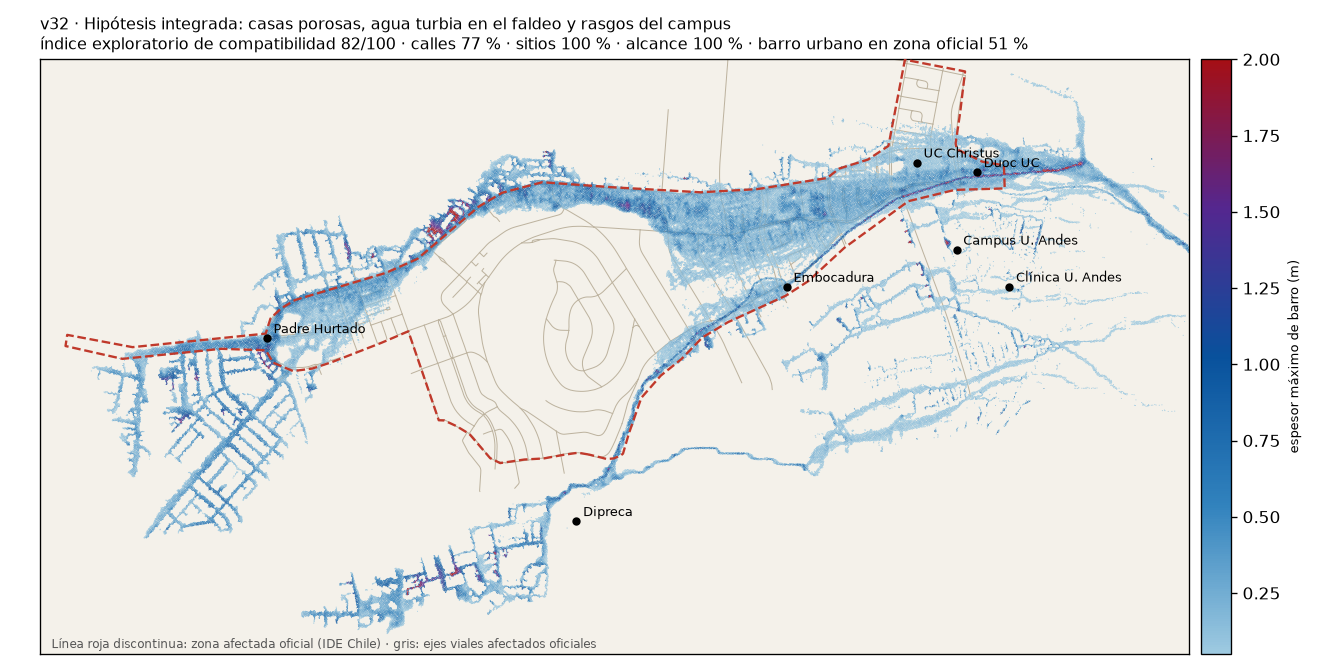
\includegraphics[width=\textwidth]{anexo/v32}\caption{Ficha v32: Hipótesis integrada: casas porosas, agua turbia en el faldeo y rasgos del campus.}\end{figure}

\paragraph{z26 · Casas porosas (paso fino).} \textbf{Qué prueba:} Que los edificios de la zona oficial dejen entrar el barro (piso a la cota del terreno más 0,3 m y alta resistencia), en vez de ser bloques macizos. \textbf{Qué muestra:} Calculado: el barro urbano dentro de la zona oficial sube de 34 \% a 54 \%; moja el 36 \% del área oficial y el 40 \% de sus predios afectados; cumple los cuatro criterios originales. Con la mitad de la resistencia (v30) casi no cambia. \textbf{Limitaciones del modelo:} El espesor calculado junto a la urgencia de la UC Christus baja a 0,30 m. El punto del campus no se moja con paso fino. \textbf{Qué levanta:} En el modelo, la retención supuesta de barro en los lotes modifica la distribución calculada dentro de la zona oficial; su representación sigue siendo un supuesto. \textbf{Estado:} IEC verificado con paso fino: 76/100 (ajuste posterior).

\begin{figure}[H]\centering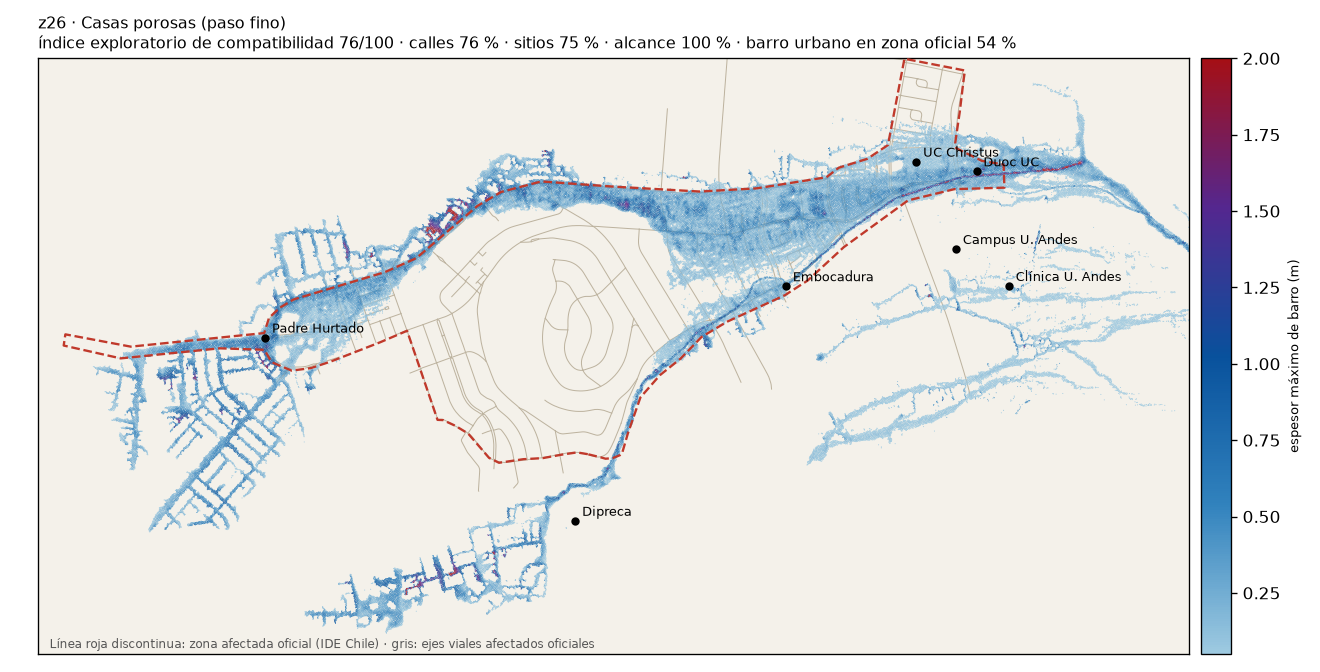
\includegraphics[width=\textwidth]{anexo/z26}\caption{Ficha z26: Casas porosas (paso fino).}\end{figure}

\paragraph{z29 · Faldeo más líquido (paso fino).} \textbf{Qué prueba:} Dos barros según la zona: Cv 0,27 en el faldeo del campus y Cv 0,43 en la rama principal, con la lluvia solo fuera de las cuencas aportantes. \textbf{Qué muestra:} Calculado: el punto de control del campus se mantiene mojado con paso fino (0,09 m), a diferencia de la hipótesis con un solo barro (0,01 m). \textbf{Limitaciones del modelo:} No reduce el barro fuera de la zona oficial: la fracción dentro de ella queda en 0,35. \textbf{Qué levanta:} En estos ensayos, un fluido supuesto más líquido en el faldeo, compatible con el agua turbia interpretada en el video de Meganoticias, produce flujo en el campus también con paso fino. \textbf{Estado:} IEC verificado con paso fino: 78/100 (ajuste posterior).

\begin{figure}[H]\centering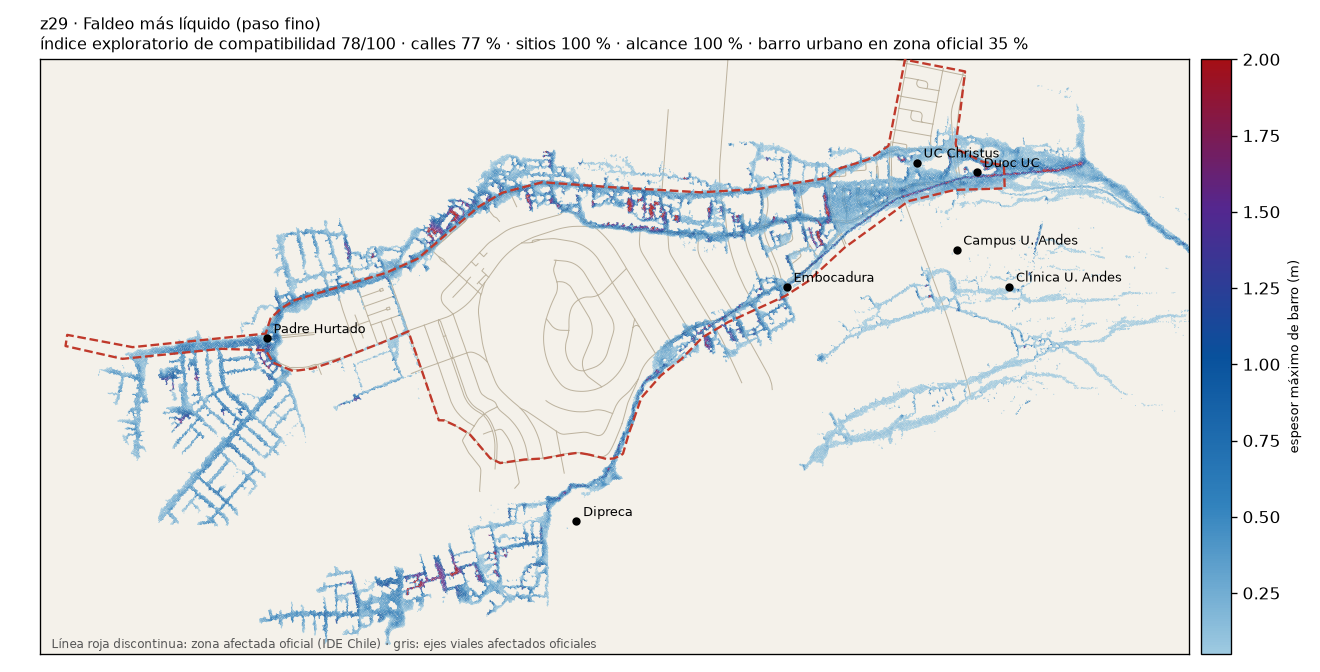
\includegraphics[width=\textwidth]{anexo/z29}\caption{Ficha z29: Faldeo más líquido (paso fino).}\end{figure}

\subsection*{Hipótesis seleccionada para la prueba reservada}

\paragraph{z02 · Cauce + brazos sur + lluvia en ladera, ciudad completa (paso fino).} \textbf{Qué prueba:} La hipótesis seleccionada antes de la prueba con observaciones reservadas: el barro sale por el cauce principal al abanico y por los brazos sur, y además se aplica una lluvia de 35 mm/h sobre la ladera quemada. Repite v02 con un paso de tiempo cuatro veces más fino para examinar la sensibilidad al paso de tiempo. \textbf{Qué muestra:} Calculado: el flujo simulado recorre los dos corredores que delimitan la zona oficial (El Alba–General Blanche y Quebrada Honda) y llega a menos de 200 m de Padre Hurtado; en el entorno de la Clínica UC Christus calcula 1,13 m (Cadena 3 informó cerca de 1 m en urgencias) y produce flujo junto a la Clínica U. de los Andes. Los indicadores coinciden con los de v02; esta comprobación numérica no valida la reconstrucción del evento. \textbf{Limitaciones del modelo:} Solo un tercio del barro simulado en zona urbana cae dentro de la zona oficial: se extiende al poniente de Padre Hurtado, por Quebrada Honda hacia Dipreca y, por la lluvia aplicada, por calles de otros barrios. No alcanza el campus de la U. de los Andes. Parte de la lluvia aplicada (unos 9.400 m$^3$) se superpone con cuencas que ya entran por los hidrogramas; v28 lo corrige. \textbf{Qué levanta:} En z02, el aporte de lluvia sobre la ladera contribuye a reproducir el flujo junto a la clínica; el resultado no establece su participación durante el evento. Como posibles explicaciones de la extensión fuera de la zona oficial se consideran la representación de los edificios, la carga gruesa y la vegetación (v25–v27). \textbf{Estado:} Hipótesis seleccionada antes de la prueba con observaciones reservadas (prueba desfavorable): IEC 72/100. Los ensayos posteriores (casas porosas, faldeo líquido, hipótesis integrada) la superan, como ajuste.

\begin{figure}[H]\centering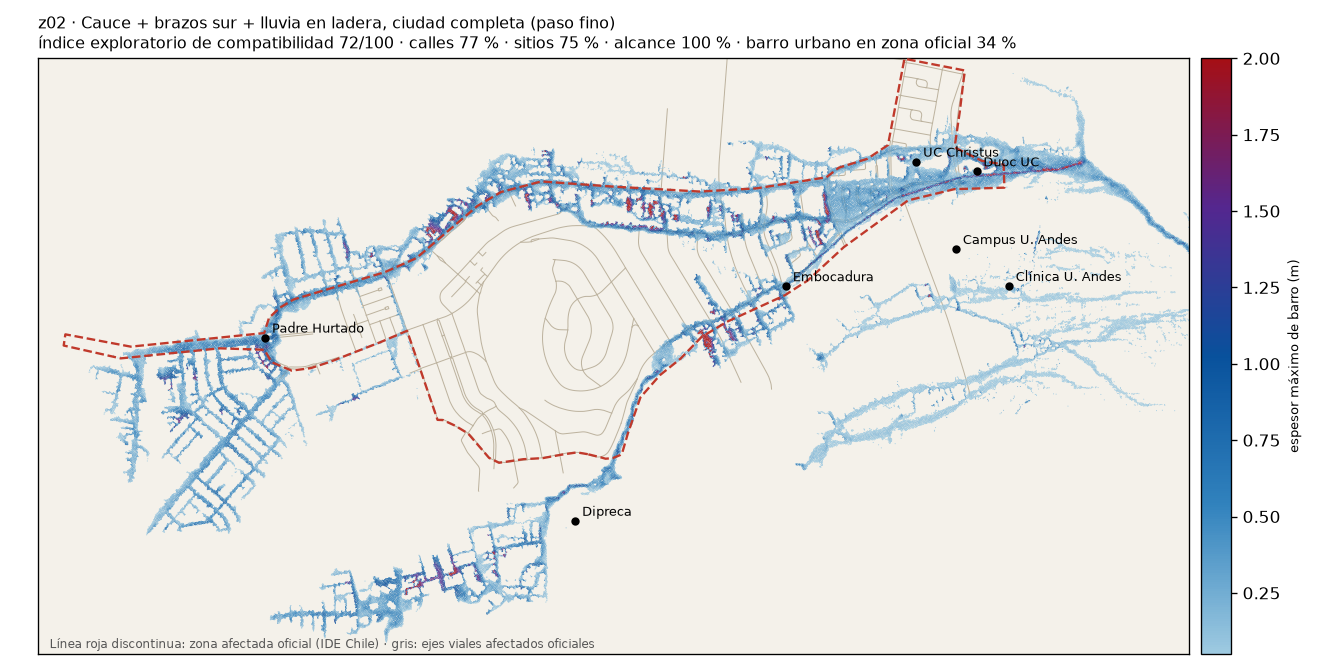
\includegraphics[width=\textwidth]{anexo/z02}\caption{Ficha z02: Cauce + brazos sur + lluvia en ladera, ciudad completa (paso fino).}\end{figure}

\subsection*{Ciudad completa}

\paragraph{v01 · Solo cauce principal, colector con capacidad nula supuesta (300 mil m$^3$).} \textbf{Qué prueba:} Todo el barro sale por el cauce principal al abanico, con los ductos de General Blanche y el colector de Bulnes Correa con capacidad nula supuesta (escenario hipotético). \textbf{Qué muestra:} Calculado: con los 42 mil edificios, el flujo se encauza por las calles; calcula 1,16 m en el entorno de la UC Christus (0,3 m con el terreno anterior), 1,9 m junto a Duoc UC, llega a 96 m de Padre Hurtado y moja Quebrada Honda. \textbf{Limitaciones del modelo:} No reproduce la afectación junto a la Clínica U. de los Andes, en La Plaza Sur ni en el campus. \textbf{Qué levanta:} Esta configuración no reproduce la afectación del sector sur. Los aportes desde ese sector constituyen una de las hipótesis consideradas para explicar la discrepancia. \textbf{Estado:} Referencia: IEC 68/100.

\begin{figure}[H]\centering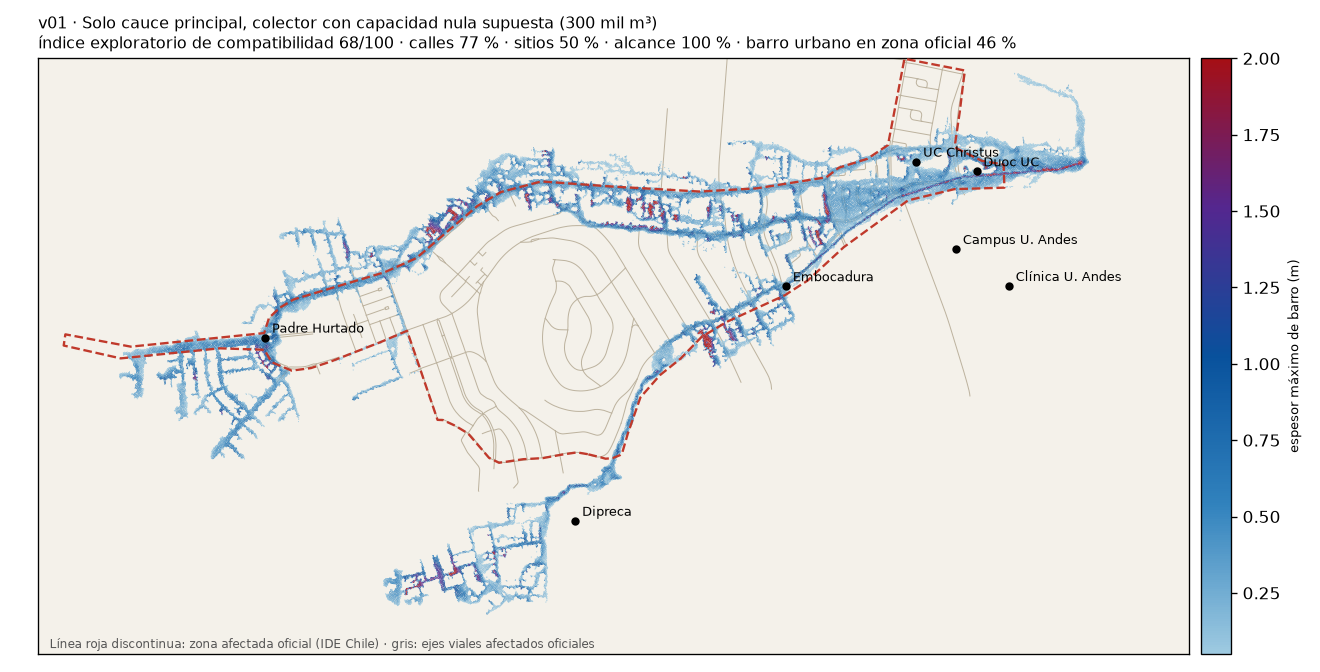
\includegraphics[width=\textwidth]{anexo/v01}\caption{Ficha v01: Solo cauce principal, colector con capacidad nula supuesta (300 mil m$^3$).}\end{figure}

\paragraph{v07 · Solo cauce principal con 150 mil m$^3$.} \textbf{Qué prueba:} Igual que v01, pero con la mitad del volumen: el valor central de la primera estimación por lluvia. \textbf{Qué muestra:} Calculado: el frente se detiene a 348 m de Padre Hurtado. \textbf{Limitaciones del modelo:} No cumple el criterio de alcance. \textbf{Qué levanta:} En los escenarios ensayados y bajo sus supuestos, unos 300 mil m$^3$ permiten reproducir el criterio de alcance; ese orden de magnitud es coherente con una estimación por lluvia que adopta la saturación del suelo informada por la autoridad. \textbf{Estado:} La configuración con el volumen bajo no cumple el criterio de alcance: IEC 67/100.

\begin{figure}[H]\centering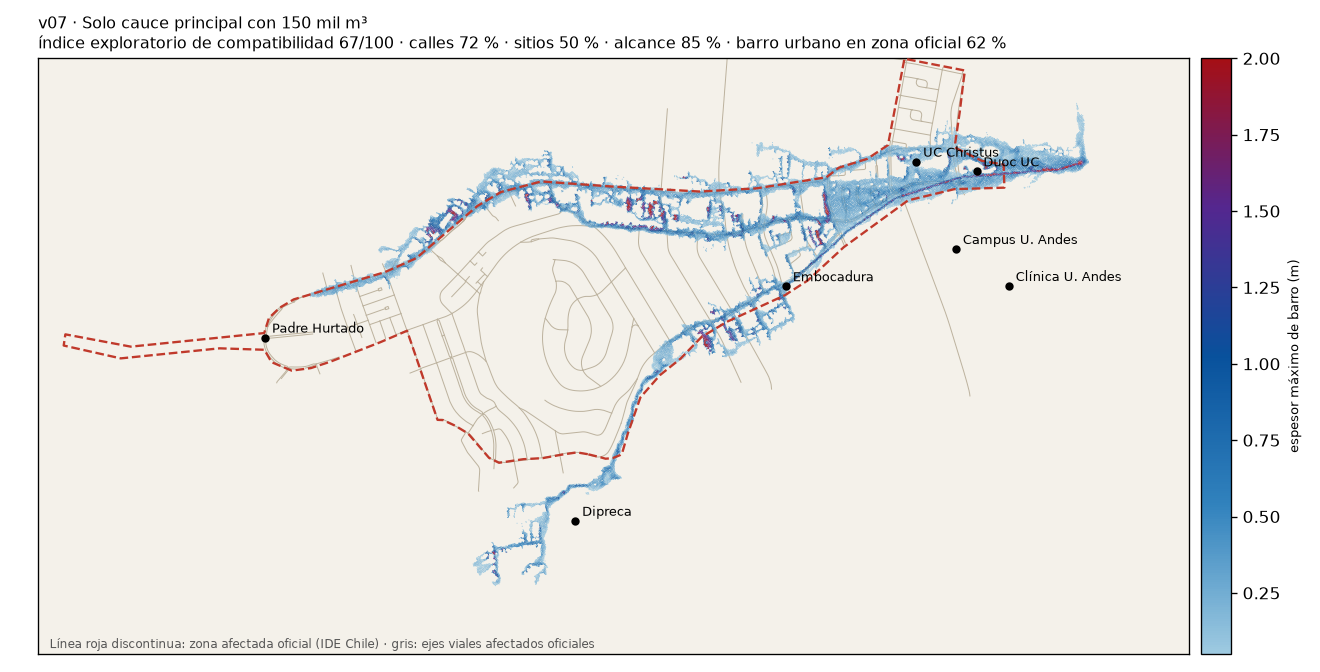
\includegraphics[width=\textwidth]{anexo/v07}\caption{Ficha v07: Solo cauce principal con 150 mil m$^3$.}\end{figure}

\subsection*{Campus U. Andes}

\paragraph{v21 · Brazo sur por el cauce oficial, sin lluvia en ladera.} \textbf{Qué prueba:} El brazo sur sigue el trazado de la red hidrográfica oficial hasta la parte alta de la Av. Álvaro del Portillo, donde termina el trazado oficial y el modelo deja salir el flujo a la avenida. Sin lluvia en la ladera, para aislar su efecto. \textbf{Qué muestra:} Calculado: el barro del brazo sur llega a la avenida (0,48 m donde termina el cauce) y baja por ella hacia La Plaza y General Blanche, de forma compatible con lo atribuido al vicerrector por Cooperativa y a Carabineros por La Tercera. \textbf{Limitaciones del modelo:} Sin la lluvia en la ladera no se reproduce la afectación junto a la Clínica U. de los Andes (0 m) y el flujo no alcanza la Biblioteca. \textbf{Qué levanta:} En las configuraciones comparadas, la lluvia sobre la ladera permite reproducir la afectación junto a la clínica, y, en el modelo, el brazo sur genera un desborde compatible con el que el vicerrector relató a Cooperativa en el costado norte del campus. \textbf{Estado:} IEC 68/100.

\begin{figure}[H]\centering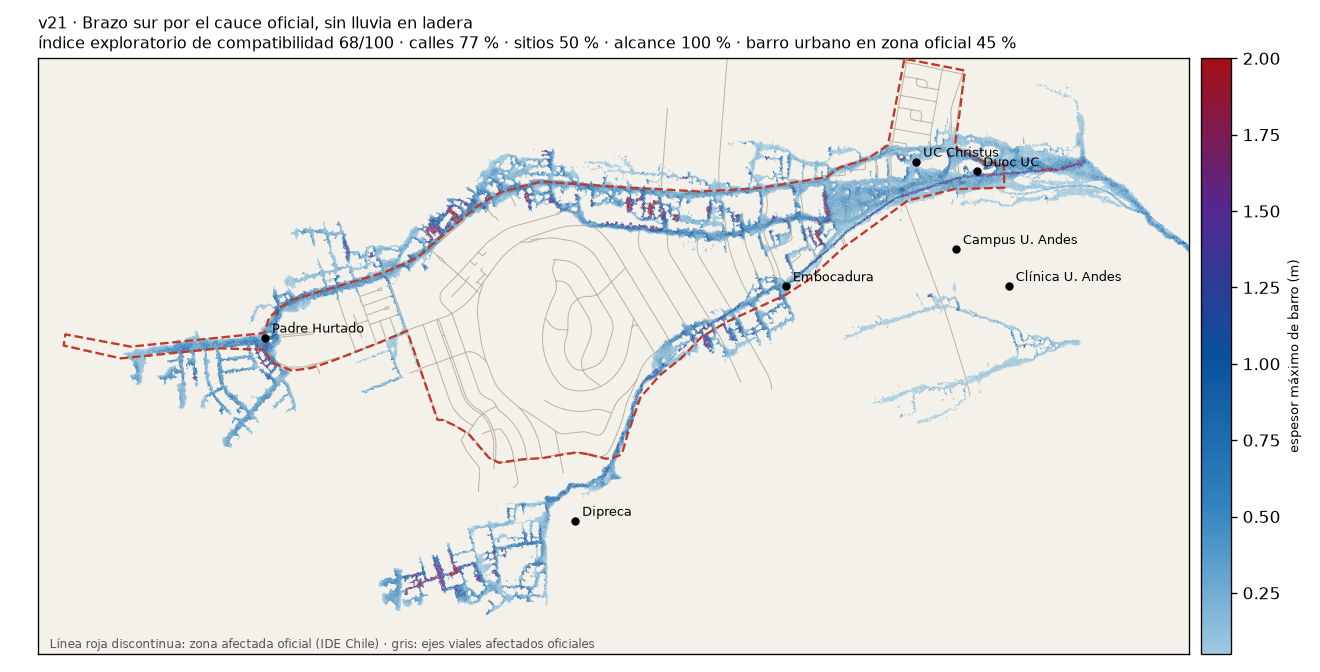
\includegraphics[width=\textwidth]{anexo/v21}\caption{Ficha v21: Brazo sur por el cauce oficial, sin lluvia en ladera.}\end{figure}

\paragraph{v19 · Brazo sur por el cauce oficial hasta Álvaro del Portillo + lluvia (paso fino).} \textbf{Qué prueba:} La hipótesis seleccionada (z02) con el brazo sur trazado según la cartografía oficial, para examinar si el flujo llega al campus y al Aula Magna. \textbf{Qué muestra:} Calculado: reproduce un desborde en la parte alta de Álvaro del Portillo y su descenso por la avenida, además de lo que logra z02. \textbf{Limitaciones del modelo:} El flujo simulado sigue por la avenida, de mayor pendiente ($\sim$8 \%) que el bosque hacia la Biblioteca ($\sim$4 \%), y no alcanza la depresión junto al edificio ni el punto de control del campus (1 cm). \textbf{Qué levanta:} En las microsimulaciones posteriores, el desborde supuesto no llega al patio con ninguno de los fluidos ensayados; el escenario más compatible supone escorrentía turbia de la ladera que, en el modelo, sigue La Plaza Sur y entra por un claro, con rasgos tallados que el relieve de 30 m no resuelve. \textbf{Estado:} IEC 71/100. Superada como ajuste por el escenario con aporte supuesto de escorrentía local (ver v32); no se determina el origen real del agua.

\begin{figure}[H]\centering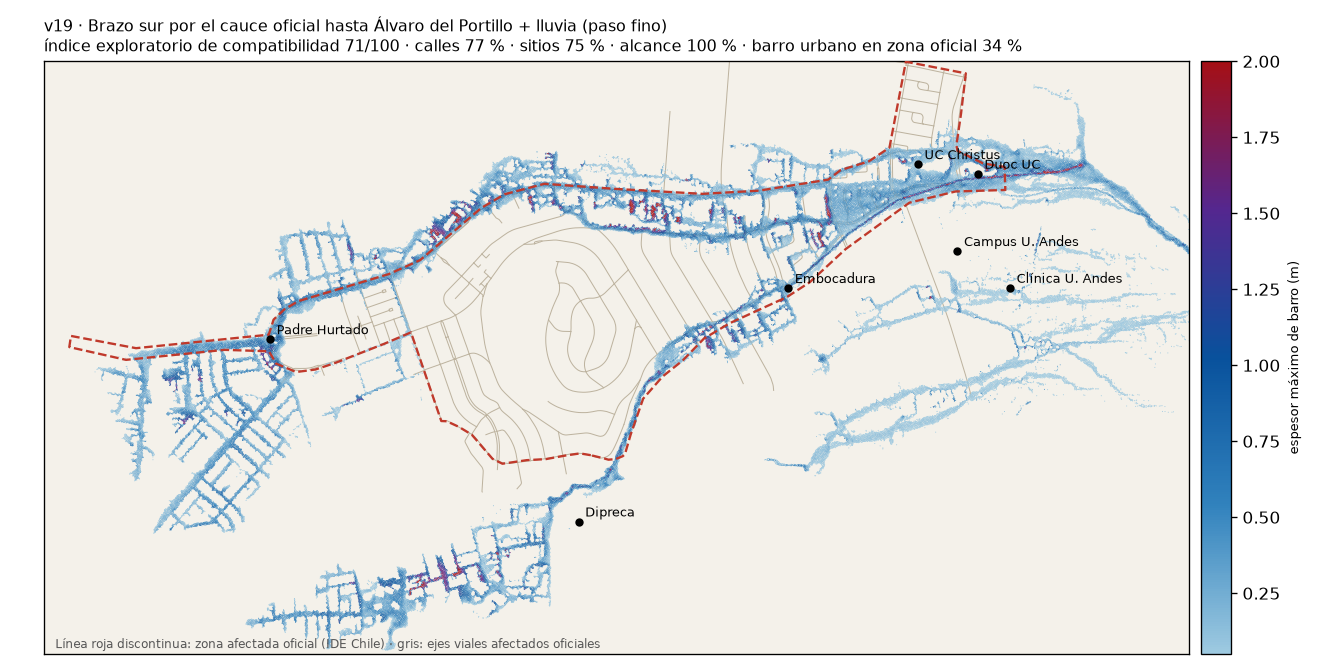
\includegraphics[width=\textwidth]{anexo/v19}\caption{Ficha v19: Brazo sur por el cauce oficial hasta Álvaro del Portillo + lluvia (paso fino).}\end{figure}

\subsection*{Colector de Bulnes Correa (escenarios hipotéticos)}

\paragraph{v17 · Escenario hipotético: capacidad supuesta del colector fijada en 30 m$^3$/s.} \textbf{Qué prueba:} Escenario hipotético con capacidad supuesta del colector fijada en 30 m$^3$/s y captura de toda la sección del cauce. No se dispuso de información pública sobre la capacidad y el estado reales del colector. \textbf{Qué muestra:} Calculado: el colector modelado alcanza la capacidad impuesta (retira 67,6 mil m$^3$ a 30 m$^3$/s) y Quebrada Honda se moja en el 62 \% de sus puntos. \textbf{Limitaciones del modelo:} — \textbf{Qué levanta:} En el modelo, con capacidad supuesta de 30 m$^3$/s, queda flujo superficial hacia Quebrada Honda. No es una evaluación de la obra real. \textbf{Estado:} Referencia inferior del intervalo explorado en estos escenarios: IEC 69/100.

\begin{figure}[H]\centering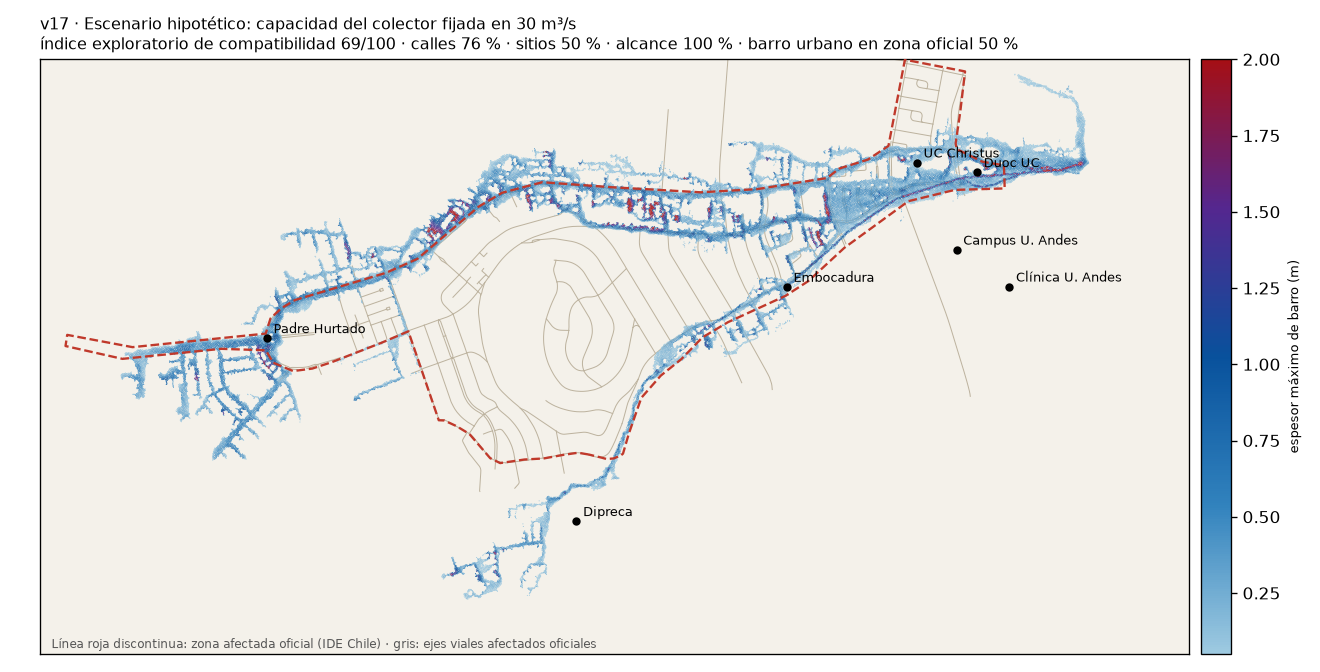
\includegraphics[width=\textwidth]{anexo/v17}\caption{Ficha v17: Escenario hipotético: capacidad supuesta del colector fijada en 30 m$^3$/s.}\end{figure}

\paragraph{v10 · Escenario hipotético: capacidad supuesta del colector fijada en 100 m$^3$/s.} \textbf{Qué prueba:} Escenario hipotético de gran capacidad con captura de toda la sección del cauce. \textbf{Qué muestra:} Calculado: el colector modelado retira unos 93 mil m$^3$ con un pico de $\sim$64 m$^3$/s y Quebrada Honda queda seca. Con 200 m$^3$/s el resultado es el mismo, porque el caudal calculado de llegada no supera $\sim$65 m$^3$/s. \textbf{Limitaciones del modelo:} El escenario no reproduce la inundación informada en Quebrada Honda; esta discrepancia no permite establecer cómo funcionó el colector real. \textbf{Qué levanta:} Bajo los supuestos ensayados y con captura completa, el análisis sitúa cerca de 65 m$^3$/s el umbral calculado de capacidad supuesta para retirar todo el flujo superficial en el modelo. Un radio de captura de 12 m dejaba pasar el flujo por el costado del sumidero: era un artefacto de representación, ya corregido. \textbf{Estado:} Referencia superior del intervalo explorado en estos escenarios: IEC 68/100.

\begin{figure}[H]\centering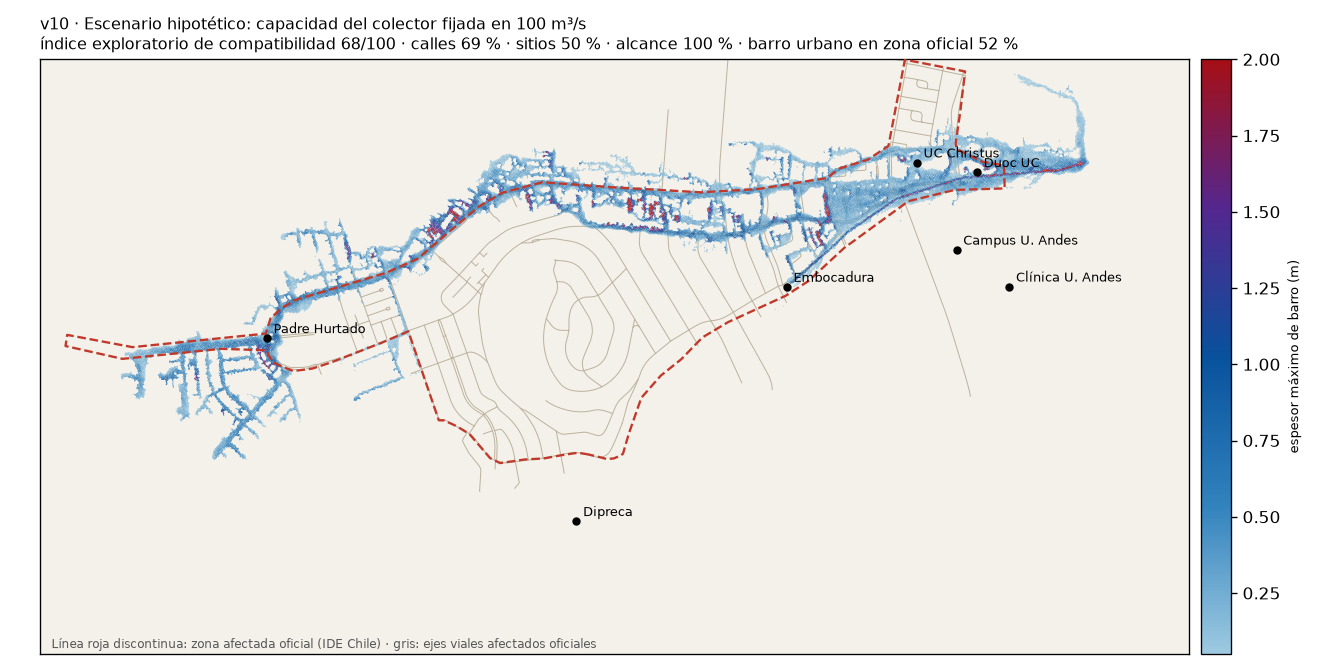
\includegraphics[width=\textwidth]{anexo/v10}\caption{Ficha v10: Escenario hipotético: capacidad supuesta del colector fijada en 100 m$^3$/s.}\end{figure}

\subsection*{Tipo de barro}

\paragraph{v08 · Barro espeso (Glenwood 1, Cv 0,45).} \textbf{Qué prueba:} Un barro más concentrado y viscoso (1.742 kg/m$^3$, fluencia 29 Pa). \textbf{Qué muestra:} Calculado: el frente se detiene a 396 m de Padre Hurtado. \textbf{Limitaciones del modelo:} No cumple el criterio de alcance. \textbf{Qué levanta:} Un material intermedio (Cv 0,43, v25) no reduce el barro fuera de la zona oficial; en todo el rango de Cv entre 0,24 y 0,48 (cuadratura de la concentración) el índice queda entre 71 y 73. \textbf{Estado:} Variante de mayor espesor: IEC 67/100.

\begin{figure}[H]\centering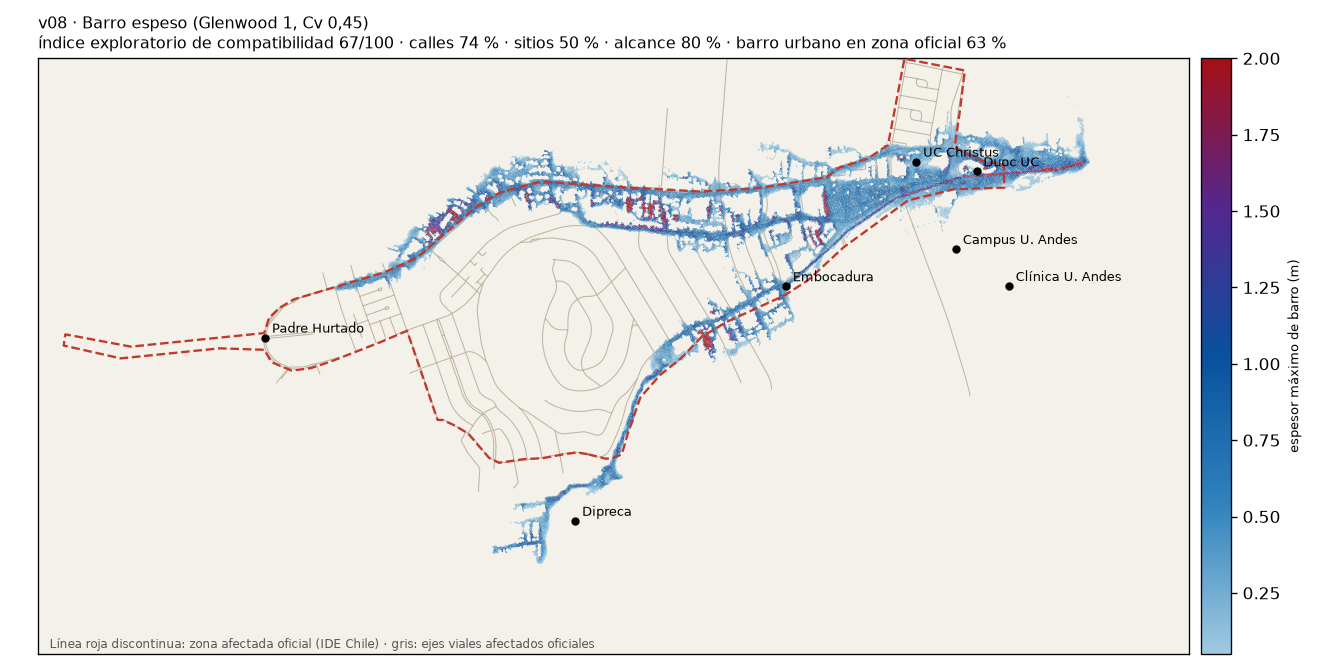
\includegraphics[width=\textwidth]{anexo/v08}\caption{Ficha v08: Barro espeso (Glenwood 1, Cv 0,45).}\end{figure}

\paragraph{v09 · Barro muy fluido (Aspen 2).} \textbf{Qué prueba:} Un barro más fluido que el de referencia. \textbf{Qué muestra:} Calculado: resultado parecido al de referencia (IEC 70/100), con algo más de barro dentro de la zona oficial. \textbf{Limitaciones del modelo:} No llega al sector sur (sin brazos sur ni lluvia). \textbf{Qué levanta:} El IEC varía poco entre los materiales ensayados; esa variación no resume por sí sola los cambios de alcance, profundidad o velocidad. \textbf{Estado:} Sensibilidad del índice al material: baja. IEC 70/100.

\begin{figure}[H]\centering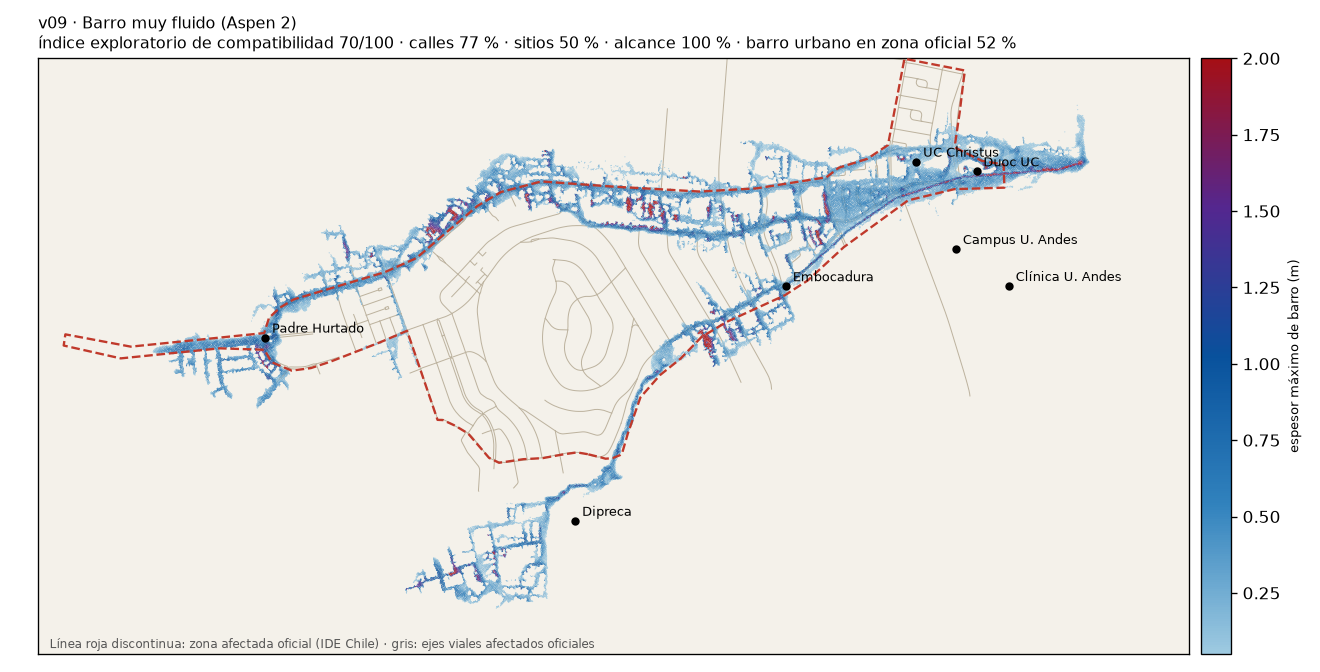
\includegraphics[width=\textwidth]{anexo/v09}\caption{Ficha v09: Barro muy fluido (Aspen 2).}\end{figure}

\subsection*{Terreno anterior (primera generación)}

\paragraph{e04 · Cauce + colector con capacidad nula supuesta, terreno con 1.103 edificios.} \textbf{Qué prueba:} La configuración seleccionada en la primera generación (9 de octubre), con solo 1.103 edificios representados y el criterio de perímetro de prensa. \textbf{Qué muestra:} Calculado: el flujo se reparte más en superficie (93 ha dentro de la zona oficial) con láminas más delgadas y llega a Padre Hurtado. \textbf{Limitaciones del modelo:} Calcula solo 0,3 m en el entorno de la UC Christus (Cadena 3 informó cerca de 1 m en urgencias). \textbf{Qué levanta:} Representar todos los edificios cambió los resultados; la representación mediante bloques impermeables podría intensificar el encauzamiento respecto de una que permita retención en edificios (v26). \textbf{Estado:} Superada por las simulaciones con la ciudad completa: IEC 68/100.

\begin{figure}[H]\centering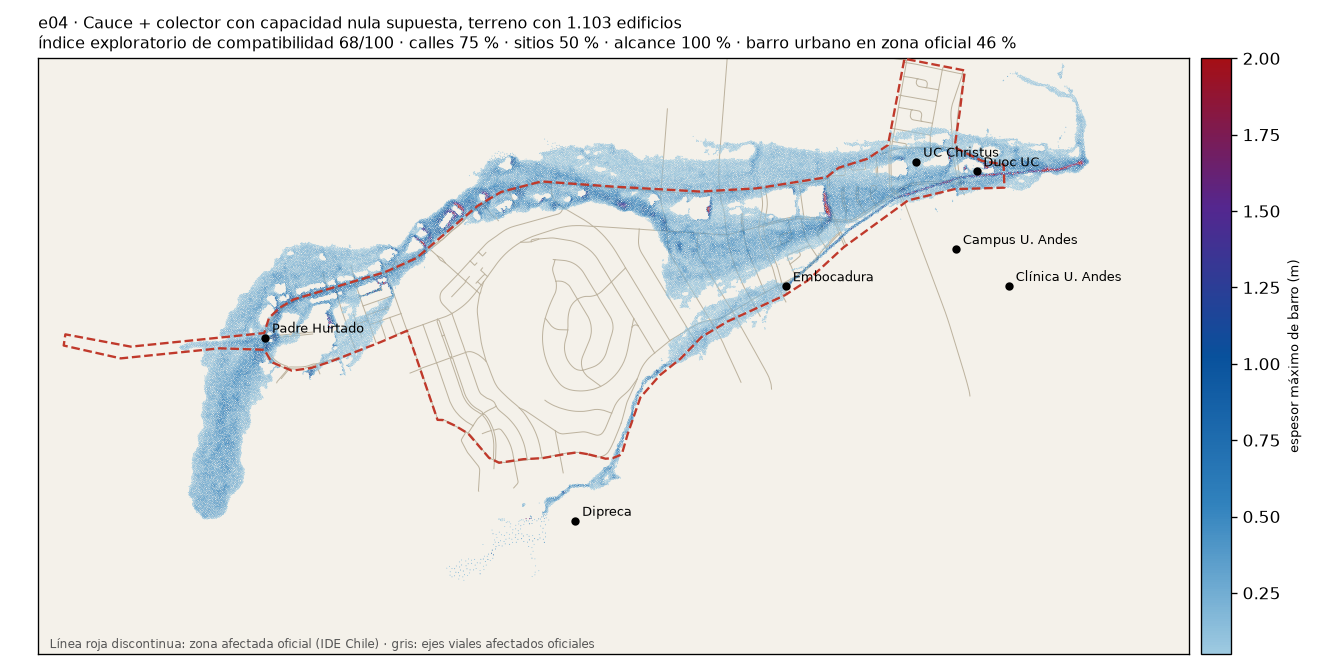
\includegraphics[width=\textwidth]{anexo/e04}\caption{Ficha e04: Cauce + colector con capacidad nula supuesta, terreno con 1.103 edificios.}\end{figure}

\paragraph{f03 · Abanico + embocadura + lluvia en ladera, terreno anterior.} \textbf{Qué prueba:} La primera simulación con lluvia sobre la ladera, con el terreno anterior. \textbf{Qué muestra:} Calculado: fue la primera en producir flujo junto a la Clínica U. de los Andes y en La Plaza Sur. \textbf{Limitaciones del modelo:} Espesor bajo en el entorno de la UC Christus y extensión fuera de la zona oficial. \textbf{Qué levanta:} Dio origen a la hipótesis seleccionada para la prueba reservada (cauce + brazos sur + lluvia, z02). \textbf{Estado:} IEC 71/100.

\begin{figure}[H]\centering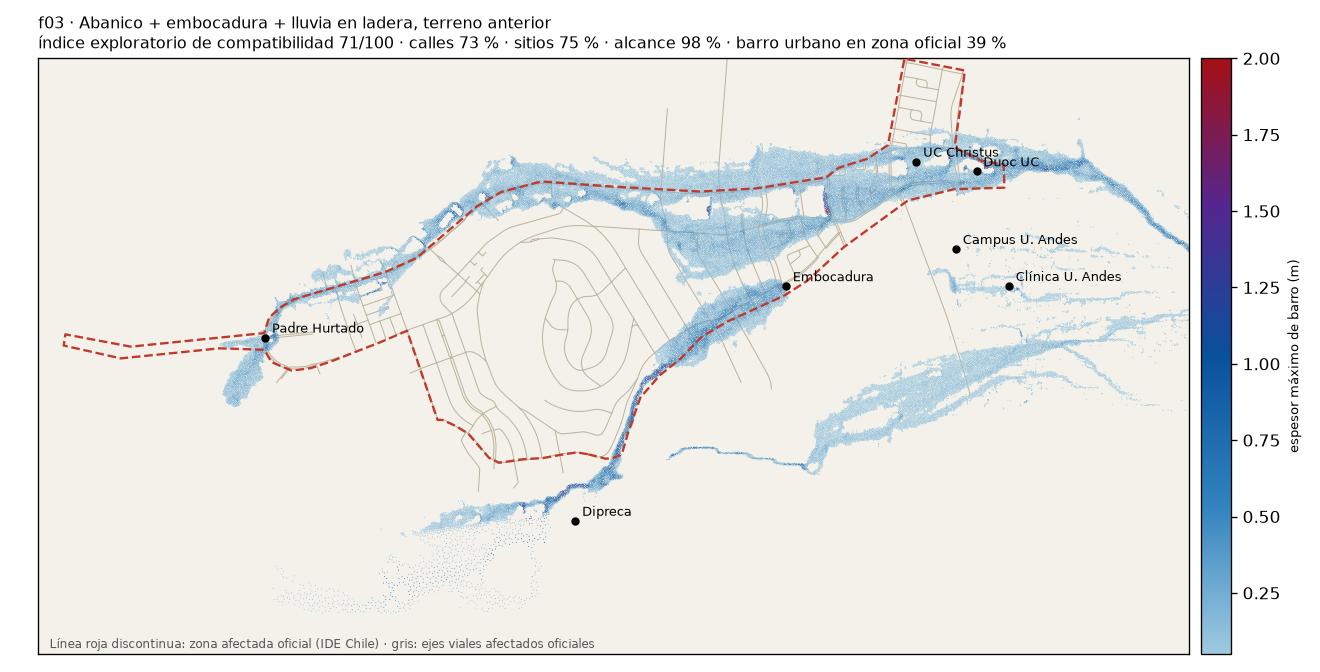
\includegraphics[width=\textwidth]{anexo/f03}\caption{Ficha f03: Abanico + embocadura + lluvia en ladera, terreno anterior.}\end{figure}

\paragraph{e03 · Solo desborde en la embocadura (H2).} \textbf{Qué prueba:} Una entrada superficial de todo el volumen supuesto en Francisco Bulnes Correa, sin inferir el funcionamiento real del canal. \textbf{Qué muestra:} Calculado: moja Quebrada Honda, pero nada del abanico. \textbf{Limitaciones del modelo:} No reproduce General Blanche, Camino El Alba, Duoc UC ni la UC Christus. \textbf{Qué levanta:} El Desconcierto recoge un desborde en Bulnes Correa informado por Carabineros. La simulación e03 no reproduce por sí sola el conjunto de observaciones. \textbf{Estado:} No reproduce por sí sola el conjunto de observaciones bajo los supuestos y el terreno de e03: IEC 16/100.

\begin{figure}[H]\centering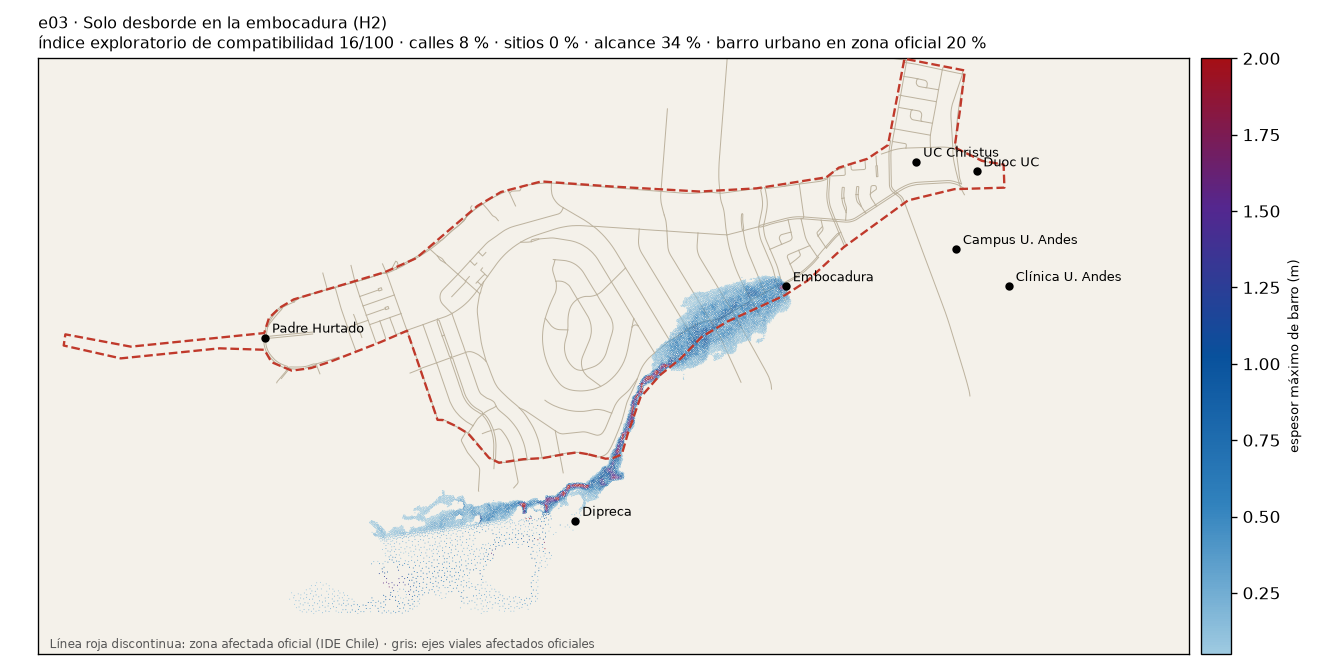
\includegraphics[width=\textwidth]{anexo/e03}\caption{Ficha e03: Solo desborde en la embocadura (H2).}\end{figure}

\end{document}
